%---------------------------------------------------------------------------%
%-                                                                         -%
%-                           LaTeX Template                                -%
%-                                                                         -%
%---------------------------------------------------------------------------%
%- Copyright (C) Huangrui Mo <huangrui.mo@gmail.com> 
%- This is free software: you can redistribute it and/or modify it
%- under the terms of the GNU General Public License as published by
%- the Free Software Foundation, either version 3 of the License, or
%- (at your option) any later version.
%---------------------------------------------------------------------------%
%->> Document class declaration
%---------------------------------------------------------------------------%
\documentclass[doublesided%,fontset=%adobe%fandol
]{Style/ucasthesis}%
%- Multiple optional arguments:
%- [<singlesided|doublesided|printcopy>]% set one or two sided eprint or print
%- [showmj]% show confidential information
%- [draftversion]% show draft version information
%- [fontset=<fandol|...>]% specify font set to replace automatic detection
%- [scheme=plain]% thesis writing of international students
%- [standard options for ctex book class: draft|paper size|font size|...]%
%---------------------------------------------------------------------------%
%->> Document settings
%---------------------------------------------------------------------------%
\usepackage[super,myhdr,list]{Style/artratex}% document settings
%- usage: \usepackage[option1,option2,...,optionN]{artratex}
%- Multiple optional arguments:
%- [bibtex|biber]% set bibliography processor and package
%- [<numbers|super|authoryear|alpha>]% set citation and reference style
%- <numbers>: textual: Jones [1]; parenthetical: [1]
%- <super>: textual: Jones superscript [1]; parenthetical: superscript [1]
%- <authoryear>: textual: Jones (1995); parenthetical: (Jones, 1995)
%- <alpha>: textual: not available; parenthetical: [Jon95]
%- [geometry]% reconfigure page layout via geometry package
%- [lscape]% provide landscape layout environment
%- [myhdr]% enable header and footer via fancyhdr package
%- [color]% provide color support via xcolor package
%- [background]% enable page background
%- [tikz]% provide complex diagrams via tikz package
%- [table]% provide complex tables via ctable package
%- [list]% provide enhanced list environments for algorithm and coding
%- [math]% enable some extra math packages
\usepackage{Style/artracom}% user defined commands
\usepackage{appendix}
\usepackage{pdfpages}
\usepackage{setspace}
\usepackage{enumerate}
\usepackage{enumitem}
%\usepackage{bicaption} % package for binary captions
%\captionsetup[figure][bi-second]{name=Figure} % the second figure caption name
%\captionsetup[table][bi-second]{name=Table} % the second table caption name
\renewcommand{\theequation}{\arabic{chapter}-\arabic{equation}}
\renewcommand{\thefigure}{\arabic{chapter}-\arabic{figure}}
\renewcommand{\thetable}{\arabic{chapter}-\arabic{table}}
\renewcommand{\contentsname}{目录\vspace{2cm}}
\renewcommand{\thesection}{\arabic{section}}

\setcounter{tocdepth}{3}           %增加目录深度
\setcounter{secnumdepth}{3}        %增加编号深度
       
%---------------此处代码为修改目录层次显示不合适问题--------      
\makeatletter
\renewcommand*\l@section{\@dottedtocline{2}{1.8em}{1.2em}}
\renewcommand*\l@subsection{\@dottedtocline{3}{3.2em}{1.2em}}
\renewcommand*\l@subsubsection{\@dottedtocline{4}{5.2em}{1.2em}}
\makeatother
%---------------------------------------------------------------------------%
%->> Document inclusion
%---------------------------------------------------------------------------%
%\includeonly{Tex/Chap_1,...,Tex/Chap_N}% selected files compilation
%---------------------------------------------------------------------------%
%->> Document content
%---------------------------------------------------------------------------%
\begin{document}
%-
%-> Frontmatter: title page, abstract, content list, symbol list, preface
%-
\frontmatter% initialize the environment
%---------------------------------------------------------------------------%
%->> Titlepage information
%---------------------------------------------------------------------------%
%-
%\includepdfmerge{[pdfname],[a-b]}//pdfname 是pdf的名字,放当前目录下,a-b是引用的页数。
%
%\includepdfmerge{lwfmmm.pdf,1}
\includepdfmerge{fengmian.pdf,1-2}
%-> Chinese titlepage
%-
\confidential{}% confidential level
\schoollogo{scale=0.95}{wzu}% university logo
%\title{在光学腔中自旋压缩态产生的研究}% 
\title[温州大学硕士学位论文]{在光学腔中自旋压缩态产生的研究}
\author{刘刚}% name of author
\advisor{王明锋}% supervisor
\advisorsec{}% co-supervisor
\degree{硕士}% degree
\degreetype{理学}% degree type
\major{凝聚态物理}% major
\institute{温州大学}% institute of author
\chinesedate{2014~年~6~月}% customized date, 6 for summer and 12 for winter graduation
%-
%-> English titlepage
%-
\englishtitle{\LaTeX{} Thesis Template\\ of \\ The University of Chinese Academy of Sciences {$~^{\pi}\pi^{\pi}$}}
\englishauthor{Huangrui Mo}
\englishadvisor{Supervisor: Professor Qingquan Liu}
\englishdegree{Master of Natural Science}% degree type <Doctor|Master> of <Philosophy|Natural Science|Engineering>
\englishthesistype{thesis}% thesis type <thesis|dissertation>
\englishmajor{Fluid Mechanics}% major
\englishinstitute{Institute of Mechanics, Chinese Academy of Sciences}
\englishdate{June, 2014}% customized date
%-
%-> Create titlepages
%-
%\maketitle
%\makeenglishtitle
%-
%-> Author's declaration
%-
\makedeclaration
%-
%-> Chinese abstract
%-

\chapter[摘要]{在光学腔中自旋压缩态产生的研究}
\vbox{}

\section*{\qquad\qquad\qquad\qquad\qquad\qquad\quad\  摘\quad 要}
\vbox{}
%\chaptermark{摘\quad 要}

\setcounter{page}{1}% set page number
\pagenumbering{Roman}% set large roman

{
	\par
	\zihao{4}
	\linespread{1.5}\selectfont
	
	
	量子光场在与原子系综相互作用的过程中产生的一系列非经典效应是近年来量子光学领域研究的一个焦点,研究这些非经典效应不仅可以帮助我们更好认识光的本质到底是什么,而且在实际的应用方面也有着很大的研究价值。量子纠缠和自旋压缩则是非常典型的两种非经典效应,它们在量子计算、量子信息处理以及精密测量等方面有着非常重要的应用。本文研究了如何在光学腔中产生自旋压缩态和量子纠缠态,主要内容包括以下两部分:
	
	1.在光学腔中自旋压缩态产生的研究。%研究了在光学腔中如何产生自旋压缩态。
	我们通过研究发现,如果将三能级原子系综置于光学腔中,然后向其内部注入一束强激光,则原子系综会在强光场和腔模共同作用下产生压缩特性。通过分析这些压缩特性我们发现其是单轴扭曲型的压缩,如果附加适当的磁场,可将单轴扭曲的哈密顿量转变成为双轴扭曲的哈密顿量,从而可以提高体系的压缩度。我们还研究了噪声对压缩过程的影响,发现即便存在噪声的情况下,体系也可以产生很高的压缩度。
	
	2.在光学腔中原子系综间纠缠态产生的研究。在同一光学腔内放入两个原子系综,通过研究表明,这两个系综会在强驱动场的作用下彼此之间建立纠缠,这一纠缠根植于原子之间的非破坏性相互作用,利用Simon的Peres-Horodecki判据证明了在这个哈密顿量下,两个原子系综之间的确存在着非经典关联。而非破坏性相互作用是连续变量量子计算中一个很重要的量子门,故我们相信本方案对量子计算的发展也起到一定的作用。
\par

\vbox{}
\keywords{量子纠缠,自旋压缩态,三能级原子系综}}
%-
%-> English abstract
%-

\chapter[Abstract]{\linespread{1.5}\selectfont RESEARCH OF GENERATION OF SPIN SQUEEZED STATES IN OPTICAL CAVITY}

\vbox{}
\section*{\qquad\qquad\qquad\qquad\qquad\quad\quad ABSTRACT}
\vbox{}
%\chaptermark{Abstract}
%\vskip 1cm


{
	\par
	\zihao{4}
	\linespread{1.5}\selectfont
	
%	 Quantum optics is a discipline that studies quantum statistics, quantum coherence properties, and quantum effects in light and matter  interactions. 
	 Recently, non-classical effects produced by interaction between quantum light field and atomic enesmbles are a focus of research in quantum optics. Studing these non-classical effects not only help us better understand what is the nature of light, but also has some great research value in practical applications. Quantum entanglement and spin squeezing are ywo typical non-classical effects, and they have very important application in quantum computing, quantum information processing, and precision measurement. This paper mainly studies how to generate spin squeezing and quantum entanglement in the optical cavity, it mainly includes the following two parts:
	 
	 1. Research on the generation of spin-squeezed states in optical cavities. We have found through   research that if a three-level atomic system is placed in an optical cavity and then a strong laser is injected into the interior, the atomic ensemble will produce spin characteristics under the action of the strong light field and the cavity mode. By analyzing these spin characteristics, we find that it is a one-axis twisting Hamiltonian. If a suitable magnetic field is added, the one-axis twisting Hamiltonian can be transformed into a two-axis twisting Hamiltonian, which can improve the squeezing degreec of the system. We also studied the effect of noise on the spin process and found that even in the presence of noise, the system can produce very high squeezing degree.

	  
	2. The study of the generation of entangled states in the atomic system in an optical cavity. Two atomic ensembles are placed in the same optical cavity. Studies have shown that the two ensembles are entangled with each other under the action of a strong driving field, which is rooted in  nondemolition interactions between atoms. Using Simon's Peres-Horodecki criterion, it is proved that there is a non-classical relationship between the two atomic ensembles under this Hamiltonian. Nondemolition interaction is a very important quantum gate in the quantum calculation of continuous variables, so we believe that this scheme also plays a certain role in the development of quantum computing.
	
	\par

\vbox{}
%\vskip 1cm
\englishkeywords{\linespread{1.5}\selectfont quantum entanglement,\  spin squeezed states,\  three-level atomic enesmble}}
%---------------------------------------------------------------------------%
% title page, abstract, dedication
{% content list region
\linespread{1.2}% local line space
%\intotoc{\contentsname}% add link to contents table and bookmark
\tableofcontents% contents catalog
\intotoc{\listfigurename}% add link to contents table and bookmark
\listoffigures% figures catalog
\intotoc{\listtablename}% add link to contents table and bookmark
\listoftables% tables catalog
}
%\chapter*{符号列表}
\chaptermark{符号列表}

\section*{字符}
\nomenclatureitem[\textbf{Unit}]{\textbf{Symbol}}{\textbf{Description}}
\nomenclatureitem[$\Unit{m^{2} \cdot s^{-2} \cdot K^{-1}}$]{$R$}{the gas constant}
\nomenclatureitem[$\Unit{m^{2} \cdot s^{-2} \cdot K^{-1}}$]{$C_v$}{specific heat capacity at constant volume}
\nomenclatureitem[$\Unit{m^{2} \cdot s^{-2} \cdot K^{-1}}$]{$C_p$}{specific heat capacity at constant pressure}
\nomenclatureitem[$\Unit{m^{2} \cdot s^{-2}}$]{$E$}{specific total energy}
\nomenclatureitem[$\Unit{m^{2} \cdot s^{-2}}$]{$e$}{specific internal energy}
\nomenclatureitem[$\Unit{m^{2} \cdot s^{-2}}$]{$h_T$}{specific total enthalpy}
\nomenclatureitem[$\Unit{m^{2} \cdot s^{-2}}$]{$h$}{specific enthalpy}
\nomenclatureitem[$\Unit{kg \cdot m \cdot s^{-3} \cdot K^{-1}}$]{$k$}{thermal conductivity}
\nomenclatureitem[$\Unit{kg \cdot m^{-1} \cdot s^{-2}}$]{$S_{ij}$}{deviatoric stress tensor}
\nomenclatureitem[$\Unit{kg \cdot m^{-1} \cdot s^{-2}}$]{$\tau_{ij}$}{viscous stress tensor}
\nomenclatureitem[$\Unit{1}$]{$\delta_{ij}$}{Kronecker tensor}
\nomenclatureitem[$\Unit{1}$]{$I_{ij}$}{identity tensor}

\section*{算子}
\nomenclatureitem{\textbf{Symbol}}{\textbf{Description}}
\nomenclatureitem{$\Delta$}{difference}
\nomenclatureitem{$\nabla$}{gradient operator}
\nomenclatureitem{$\delta^{\pm}$}{upwind-biased interpolation scheme}

\section*{缩写}
\nomenclatureitem{CFD}{Computational Fluid Dynamics}
\nomenclatureitem{CFL}{Courant-Friedrichs-Lewy}
\nomenclatureitem{EOS}{Equation of State}
\nomenclatureitem{JWL}{Jones-Wilkins-Lee}
\nomenclatureitem{WENO}{Weighted Essentially Non-oscillatory}
\nomenclatureitem{ZND}{Zel'dovich-von Neumann-Doering}

% list of symbols, preface content
%-
%-> Mainmatter
%-
\mainmatter% initialize the environment
%---------------------------------------------------------------------------%
%->> Main content
%---------------------------------------------------------------------------%

\chapter{绪论}\label{chapter1}
\vbox{}\vbox{}
\section{引言}\label{section11}
\vbox{}
近些年来,量子信息\cite{bennett1993teleporting,bennett1992communication,bennett1984proceedings,beige2001secure}和量子计算\cite{shor1994proc,nielsen2002quantum,ekert1996quantum}研究领域的兴起正引起人们的浓厚兴趣,因为其在人们生活中有着很重要的应用。量子信息和量子计算之所以备受人们的青睐,主要在于它们拥有一些经典通信和计算所不具备的特性,比如量子算法和量子隐形传态等\cite{bennett1992communication},而这些功能的实现,与量子纠缠有着密切的联系。能够在理论上研究清楚量子纠缠到底是什么,这已经成为这个领域的一个核心问题。从1935年EPR佯谬\cite{einstein1935can}和薛定谔的猫以来\cite{article1935},无论是实验物理学家还是理论物理学家他们对量子纠缠的研究都非常的感兴趣。量子纠缠之所以这么“受欢迎”,主要是因为它有一些经典关联所没有的特性,而正因为这些特性存在所以使得量子纠缠在量子隐形传态和量子计算等方面都占有核心地位。但是截至目前为止如何有效的描述量子纠缠一直都显得格外的困难,这与量子纠缠的特殊性有着很重要的关系。目前已有的比较成功的描述两qubit纠缠的量是所谓的并发度(concurrence)\cite{article1997,PhysRevA.68.012101}描述,但是对于多体纠缠的描述一直以来都没有找到一个好的解决方案。

除了其在量子通信和计算方面的用途以外,科学家们还发现利用纠缠可以提高量子精密测量的测量精度,他们在研究干涉仪和原子钟等问题的时候,发现了一种可以能够使实验上相位和频率的测量相对于无关联态时提高的态,通过研究表明其正是我们接下来要讲的自旋压缩态,我们用自旋压缩参数来描述它。

由于当时对纠缠的认识上的欠缺,因而并没能特别指出自旋压缩态和纠缠之间的关系。后来随着研究的进一步的深入,人们发现自旋压缩和纠缠之间有着一种天然的联系,而自旋压缩参数除了用来描述自旋压缩之外,还可以用来判据纠缠。自旋压缩参数较其它的纠缠判据(如并发度)相比有如下的优点:首先,自旋压缩参数的定义与角动量算符的平均值和涨落性质有关,因而有比较清晰的物理图像;其次,自旋压缩态与量子精密测量和原子钟等之间有着十分紧密的关系,因而有更加实际的应用。

\vbox{}
\section{自旋压缩理论的研究背景}\label{section12}
\vbox{}
压缩态概念的最早出现是Earle Kennard在1927年发表的论文\cite{Kennard1927}(尽管当时没有创造出压缩态),他在海森堡不确定关系的约束下处理了谐波振子的一般高斯波包的演化,从而产生了压缩态。后来Stoler在前人的基础上于1970年提出了光场压缩态的概念\cite{stoler1970equivalence}。1976年,Yuen在研究了压缩态光场的量子特性\cite{yuen1976two}以后提出了双光子相干态的概念,实质是压缩态。
人们在研究光场压缩性质的时候,自然而然的就想到在光与原子系综相互作用的系统中,原子系综是不是也会出现压缩性质?于是人们开始了对原子压缩的研究。

1981年,Walls和Zoller第一次将光场压缩的概念推广到原子系统中\cite{PhysRevLett.47.709},引入了原子偶极压缩的概念。后来人们对原子系综的压缩进行了不断深入的研究,结果发现在自旋系统或角动量系统中也有着类似的压缩性质存在,于是自旋压缩态的研究正式拉开序幕。

1992年,Wineland等人\cite{PRA1992Wineland}发现,当原子系综处于压缩态的时候,其系统的量子噪声会减少,从而可以提高光谱的灵敏度,由于这个现象和光场压缩态的很相似,所以相应的量子态就叫做原子的自旋压缩态。后来研究表明,要想在一个集体自旋系统中产生自旋压缩态,则一定要有非线性耦合才可以,因为线性耦合只是对系统进行一个旋转操作。

1993年,Kitagawa和Ueda\cite{PRA1993Kitagawa}在理论上利用两个典型的非线性耦合(单轴扭曲和双轴扭曲)产生了自旋压缩态。自此以后,一些其他的产生自旋压缩态方法也相继被提出。系统能够实现自旋压缩也就意味着系统中存在着纠缠,同时也就意味着可以实现更高精度的测量,因而如何产生自旋压缩态在量子信息和量子计算中也有着非常重要的意义。

2002年,S\o{}rensen和M\o{}lmer等人\cite{PRA2002SS}通过将大量铷原子放在坏腔中利用光与原子相互作用产生自旋压缩态。研究表明,由于原子衰变和腔损失引起的粒子之间的量子相关性的损失可以通过在大量原子系统中的强非线性耦合来平衡,所以在坏腔与场的耦合中有可能观察到显著的原子自旋压缩。2010年,Anne Louchet-Chauvet等人\cite{LCA2010}使用量子非破坏性测量的方法来产生自旋压缩态,并在$10^5$个冷铯原子云中形成纠缠。他们的实验方案较之前的原子投影噪声极限相比,其信噪比提高了1.1dB。2017年,J. Borregaard等人\cite{NJP2017J-Borregaard}在\cite{PRA2002SS}的基础上,另外加了两束激光,利用强光控制弱光的方法将系统的哈密顿量就变成了一个双轴扭曲的哈密顿量,此时产生了较前面方案更强的自旋压缩态。

以上各方法作为自旋压缩态的产生研究对量子信息的发展都起到了很大的推动作用,但作为本论文的选题,需要对其的优缺点进行分析和评价,然后选择一个合适的突破点作为本论文的切入点。在光学腔中利用光与原子相互作用来产生自旋压缩的方案最为成熟,但是已有的理论方案过于复杂,由于量子系统的特殊性,方案过于复杂不利于在实验中产生较纯压缩度较高的自旋压缩态。于是进一步的改进并简化理论方案,优化处理物理过程的数学手段,成了其发展过程至关重要的一个环节。

\vbox{}
\section{自旋压缩态的主要应用}\label{section13}
\vbox{}
自旋压缩态(Squeezed spin states)是集体自旋的纠缠量子态,由于海森堡不确定关系给测量仪器设置了标准量子极限,无论测量仪器多么精密,误差始终存在,但是处于自旋压缩态的原子系综的两个不对易的相互正交的自旋分量可以在不违反海森堡不确定度关系的前提下,通过增大一个自旋分量的涨落来降低另外一个与之不对易的自旋分量的量子涨落从而使其低于真空涨落,这就使得自旋压缩态研究变得至关重要。由于产生自旋压缩的具体系统的不同,所以自旋压缩的定义并不唯一,相应也有许多不同的应用,主要包括两个方面:

自旋压缩的一个主要应用是用来检测量子纠缠,量子纠缠在量子物理学的基础和量子信息处理中都起着关键作用。 参数$\xi_s^2$与负成对关联和并发度相关,可以表征一类多体自旋1/2态的成对纠缠。自旋压缩参数是多体纠缠的证据判据。

自旋压缩的另一个应用,是在实验中提高测量的精度,例如在Ramsey光谱学中,以及制造更精确的原子钟和重力波干涉仪。 因此,许多努力都致力于在原子系统中实现压缩。 这些工作基本上可以分为两类:通过原子-光子相互作用在原子系综中产生自旋压缩和通过原子碰撞在BEC中产生自旋压缩。

\vbox{}
\section{本文研究的内容}\label{section14}
\vbox{}
本文的研究主要围绕在光学腔中$\Lambda$型原子与量子光场相互作用的问题展开,研究了原子系综在经典光场的驱动下,其压缩性质的变化以及不同原子系综之间纠缠的的产生问题。

第一章,我们先介绍了自旋压缩态的研究背景、研究意义、研究现状及其它的主要应用,然后介绍了本文的安排。

第二章,我们介绍了与本文有关的一些基本理论知识。首先介绍了光场的量子化,光与原子的相互作用等,然后我们介绍了自旋压缩态的概念、判据以及产生等知识,再后我们也介绍了关于纠缠的一些理论,包括纠缠的概念、纠缠的分类以及应用,最后我们也介绍了海森堡朗之万理论的知识。

第三章,我们提出了在腔QED系统中通过一个非共振受激拉曼过程来制备原子系综自旋压缩态的理论方案。原子系综在光场的驱动下,通过选取合适的参数得到了一个OAT型的有效哈密顿量,随后我们研究了在噪声的影响下这个哈密顿量是如何支配系统的演化的,在得出演化方程以后我们分析了系统的压缩特性,通过分析表明我们的方案可以获得不菲的压缩度。我们通过添加一个沿极化方向的磁场发现可以将OAT压缩转变为TAT压缩,虽然压缩度有所提高,但其对噪声的影响也更加敏感。

第四章,我们提出了利用相干光场来制备原子系综纠缠态的方案。该方案是基于置于光学腔中的原子系综被相干光场驱动,利用腔模的“量子公共汽车”效应来建立起原子之间的非经典关联的研究。两个原子系综在相干光场的驱动下,通过将得到的系统哈密顿量消除激发态从而得到有效哈密顿量,然后在Holstein-Primakoff近似下,定义新的原子算符,并计算出了其在系统哈密顿量作用下随时间的演化方程。利用Simon的Peres-Horodecki判据我们证明了在这个哈密顿量支配下,两个原子系统之间的确有纠缠发生。我们也分析了存在噪声的情况下我们方案的性能。

第五章,我们对全文的一个总结与展望。





%具体以单模光场与多个原子相互作用的模型为例,我们首先研究了在光学腔中量子光场与原子之间通过非共振受激拉曼过程可以产生自旋压缩态,随后我们详细的分析了原子系综中自旋压缩的动力学特性,并分析了自旋压缩的一些特性。随后我们在同样的光学腔中通过光与原子相互作用建立了两个原子子系统之间的纠缠,并分析了纠缠结果。本文共分为六章,各章内容介绍如下:

% 在这一部分我们主要研究了同样在光学腔中如何在两个原子系综的子系统之间建立纠缠的问题。我们研究发现,在光学腔内部放入两堆原子(系综),则这两个系综会在强的驱动场的作用下彼此之间会建立起纠缠。我们先写出了系统的哈密顿量,然后在大失谐的情况下绝热消除掉激发态,最后我们得到了在某个旋转框架下的哈密顿量,在Holstein-Primakoff近似下,我们定义了新的原子算符,并计算出了其在系统哈密顿量的作用下随时间的演化。我们利用Simon的Peres-Horodecki判据证明了在我们的这个哈密顿量下,两个子系统之间的确有纠缠发生。我们希望我们的方案能够在量子信息或量子计算的发展进程中起到一点积极的意义。


%主要研究了在光学腔中如何产生自旋压缩态。我们通过研究表明,如果将三能级原子系综置于光学腔中,然后向其内部注入一束强激光,则原子系综会在强光场和腔模共同作用下产生压缩特性。
%通过分析这些压缩特性我们发现其是单轴扭曲型的压缩,附加适当的磁场可以将单轴扭曲的哈密顿量转变成双轴扭曲的哈密顿量,从而可以提高系统的压缩度。我们还分析了噪声对系统的影响,发现即便在存在噪声的情况下,系统也可以产生很高的压缩度。

%研究了在光学腔中如何建立两个原子系综之间的纠缠。在同一光学腔内放入两个原子系综,通过研究表明,在光学腔内部放入两个原子系综,则这两个系综会在强驱动场的作用下彼此之间建立纠缠。这一纠缠根植于原子之间的非破坏性相互作用,利用Simon的Peres-Horodecki判据证明了在这个哈密顿量下,两个原子系综之间的确存在着非经典关联。而非破坏性相互作用是连续变量量子计算中一个很重要的量子门,故我们相信本方案对量子计算的发展也起到一定的作用。





%第一章,简要的介绍了一下自旋压缩理论的研究背景,研究进展以及它的主要应用。第二章,主要系统地介绍了一些与本文相关的理论知识。第三章,详细介绍了自旋压缩的定义,自旋压缩的判据以及纠缠的相关知识。第四章,我们研究了在光学腔中通过非共振的受激拉曼过程来实现OAT和TAT的自旋压缩。第五章,我们研究了如何在光学腔中通过光与原子相互作用来产生两个原子系综之间的纠缠。第六章,是对本文的总结与展望。



\chapter{基本理论}\label{chapter2}
\vbox{}\vbox{}

本章主要介绍与本文有关的一些理论背景知识。在第一节我们先从光场的量子化开始介绍了光与原子的相互作用等知识,然后第二节我们介绍了自旋压缩态的概念、判据以及产生等知识,再后第三节我们也介绍了关于纠缠的一些理论,包括纠缠的概念、纠缠的分类以及应用,最后第四节我们也介绍了海森堡朗之万理论的知识。
%第一节先介绍一下光场量子化的理论知识。第二节介绍光场与物质相互作用的理论知识。第三节介绍与海森堡-朗之万理论相关的一些理论知识。第四节则简单了介绍了一下腔QED相关的理论知识。
%光与物质的相互作用是量子光学里最基本的问题之一,单模电磁场与二能级原子的相互作用是电磁场与原子相互作用最简单、最基本的相互作用形式。本节以单模光场与二能级原子的相互作用为例,第一小节介绍原子与场相互作用系统的哈密顿量,第二小节介绍单模光场与二能级原子相互作用的半经典理论,第三小节介绍单模光场与二能级原子相互作用的全量子理论。
\vspace{1cm}
\section{光与原子相互作用}
\vspace{1cm}
\subsection{光场的量子化}
为了量化自由空间中的电磁场,可以方便地从基于麦克斯韦方程的场的经典描述开始。下面的这些方程分别将电场强度$\bm{E}$和磁场强度$\bm{H}$与电位移矢量和磁感应矢量$\bm{D}$和$\bm{B}$相关联,在真空中麦克斯韦方程组\cite{pennarun2007tripartite}的表现形式为(在mks单位下)
\begin{align}
\nabla  \times \bm{ H} &=    \frac{{\partial \bm{ D}}}{{\partial t}},\label{eq1}\\
\nabla  \times \bm{ E} &=  - \frac{{\partial \bm{ B}}}{{\partial t}},\label{eq2}\\
\nabla  \cdot  \bm{ B} &= 0,\label{eq3}\\
\nabla  \cdot  \bm{ D} &= 0,\label{eq4}
\end{align}
它们之间满足
\begin{align}
\bm{ B} &= {\mu _0}\bm{H},\label{eq5}\\
\bm{ D }&= {\epsilon_0}\bm{ E},\label{eq6}
\end{align}
其中$\epsilon_0$和$\mu_0$分别是自由空间的介电常数和磁导率,与光速$c$之间的关系为${\mu _0}{\epsilon_0} = {c^{ - 2}}$。下面,对方程(\ref{eq2})两边取旋度,使用方程(\ref{eq1})和(\ref{eq4}-\ref{eq6})可得电场强度$\bm{E}(\bm{r},t)$满足的波动方程
\begin{align}
	{\bm{\nabla} ^2}\bm{E} - \frac{1}{{{c^2}}}\frac{{{\partial ^2}\bm{E}}}{{\partial {t^2}}} = 0,\label{eq7}
\end{align}
其中,使用了关系式$\bm{\nabla } \times \left( {\bm{\nabla}  \times \bm{E}} \right) = \bm{\nabla } \cdot \left( {\bm{\nabla } \cdot \bm{E}} \right) - {\bm{\nabla} ^2}E$。

我们首先考虑电场具有适合于长度为L的空腔谐振器的空间依赖性。我们将电场在$x$方向上线性极化并在空腔的一般模式下展开
\begin{align}
{E_x}\left( {z,t} \right) = \sum\limits_j {{A_j}{q_j}\sin \left( {{k_j}z} \right)} ,\label{eq8}
\end{align}
其中
\begin{align}
{k_j} &= \frac{{j\pi }}{L},j = 1,2,3,...,\label{eq9}\\
{A_j} &= {\left( {\frac{{2v_j^2{m_j}\pi }}{{V{_0}}}} \right)^{1/2}},\label{eq10}
\end{align}
其中${v_j} = j\pi c/L$是腔的本征频率,$V$是谐振腔的体积,${m_j}$是一个与质量有关的常数,${q_j}$是位置坐标。同样,可将磁场模式化展开
\begin{align}
{H_y}\left( {z,t} \right) = \sum\limits_j {{A_j}\left( {\frac{{{{\dot q}_j}{_0}}}{{{k_j}}}} \right)\cos \left( {{k_j}z} \right)} ,\label{eq11}
\end{align}
电磁场的经典哈密顿量为
\begin{align}
H = \frac{1}{2}{\smallint _V}d\tau \left( {{_0}E_x^2 + {\mu _0}H_y^2} \right),\label{eq12}
\end{align}
其中积分为对整个腔体积分。将式(\ref{eq8})和式(\ref{eq11})代入式(\ref{eq12})中,我们得到
\begin{align}
H = &\frac{1}{2}\sum\limits_j {\left( {{m_j}v_j^2q_j^2 + {m_j}\dot q_j^2} \right)} \nonumber\\
= &\frac{1}{2}\sum\limits_j {\left( {{m_j}v_j^2q_j^2 + \frac{{p_j^2}}{{{m_j}}}} \right)} ,\label{eq13}
\end{align}
式中${p_j} = {m_j}{\dot q_j}$是第$j$个腔模的正则动量。

为了将光场量子化,我们引入了两个算符$p_j$和$q_j$,它们满足对易关系
\begin{align}
\left[ {{q_j},{p_{j'}}} \right] = i\hbar {\delta _{jj'}},\label{eq14}\\
\left[ {{q_j},{q_{j'}}} \right] = \left[ {{p_j},{p_{j'}}} \right] = 0,\label{eq15}
\end{align}
为了方便起见,我们再引入两个新算符$a_j$和$a_j^\dagger$
\begin{align}
{a_j}{e^{ - i{v_j}t}}& = \frac{1}{{\sqrt {2{m_j}\hbar {v_j}} }}\left( {{m_j}{v_j}{q_j} + i{p_j}} \right),\label{eq16}\\
a_j^\dag {e^{i{v_j}t}}& = \frac{1}{{\sqrt {2{m_j}\hbar {v_j}} }}\left( {{m_j}{v_j}{q_j} - i{p_j}} \right),\label{eq17}
\end{align}
接下来,$a_j$和$a_j^\dagger$的表达式代入式(\ref{eq13}),则哈密顿量变为
\begin{align}
H = \hbar {\rm{ }}\sum\limits_j {{v_j}\left( {a_j^\dag {a_j} + \frac{1}{2}} \right)} ,\label{eq18}
\end{align}
$a_j$表示系统的湮灭算符,$a_j^\dagger$表示系统的产生算符,当算符$a_j$作用在量子系统的态上时,系统湮灭一个光子,当算符$a_j^\dagger$作用在量子系统的态上时,系统产生一个光子。由算符$p_j$和$q_j$所满足的对易关系易式我们可以轻易地推导出$a_j$和$a_j^\dagger$满足的对易关系为
\begin{align}
\left[ {{a_j},a_{j'}^\dag } \right]& = {\delta _{jj'}},\label{eq19}\\
\left[ {{a_j},{a_{j'}}} \right] &= \left[ {a_{j}^\dag ,a_{j'}^\dag } \right]{\rm{ = }}0,\label{eq20}
\end{align}
将$a_j$和$a_j^\dagger$代入方程(\ref{eq8})和方程(\ref{eq11})可以得到由$a_j$和$a_j^\dagger$描述的电磁场表达式为
\begin{align}
{E_x}\left( {z,t} \right) &= \sum\limits_j {{\varepsilon _j}\left( {{a_j}{e^{ - i{v_j}t}} + a_j^\dag {e^{i{v_j}t}}} \right)\sin \left( {{k_j}z} \right)} ,\label{eq21}\\
{H_y}\left( {z,t} \right) &=  - i{_0}c\sum\limits_j {{\varepsilon _j}\left( {{a_j}{e^{ - i{v_j}t}} - a_j^\dag {e^{i{v_j}t}}} \right)\cos \left( {{k_j}z} \right)} ,\label{eq22}
\end{align}
其中${\varepsilon _j} = \left( \hbar v_j /\epsilon_0 V\right)^{1/2}$。

以上讨论的电磁场是处于一维有限腔中的情况,如果将一维腔拓展成为三维腔,其结果将变为如下的形式
\begin{align}
\bm{ E}\left( {\bm{ r},t} \right)& = \sum\limits_{\bm{ k}} {{{\hat\epsilon }_{\bm{ k}}}{\epsilon_{\bm{ k}}}{a_{\bm{ k}}}{e^{ - i{v_{k}}t + i\bm{ k} \cdot\bm{r}}} + H.c.} ,\label{eq23}\\
\bm{ H}\left( {\bm{ z},t} \right)& = \frac{1}{{{\mu _0}}}\sum\limits_{\bm{ k}} {\frac{{\bm{ k} \times {{\hat \epsilon}_{\bm{ k}}}}}{{{v_k}}}{\varepsilon _{\bm{ k}}}{a_{\bm{ k}}}{e^{ - i{v_k}t + i\bm{ k} \cdot \bm{r}}} + H.c.} , \label{eq24}
\end{align}
其中$H.c.$表示厄米共轭,$\bm{ k}$为波矢,有$\bm{ k}{\rm{ = }}\frac{{2\pi }}{L}\left( {{{\bm{ e}}_x}{n_x} + {{\bm{ e}}_y}{n_y} + {{\bm{ e}}_z}{n_z}} \right)$,其中$n_x,n_y,n_z =  \pm 1, \pm 2, \pm 3,...$,${\hat \epsilon_{\bm{ k}}}$为单位极化矢量,由方程(\ref{eq4})可以得到$\bm{k} \cdot {\hat \epsilon_{\bm{ k}}} = 0$,所以对于每个$\bm{k}$有两个独立的极化方向。

\subsection{原子-场相互作用的哈密顿量}\label{subsection21}

一个电量为$e$,质量为$m$的电子受到电磁场的作用,可以用如下的哈密顿量描述
\begin{align}
H = \frac{1}{{2m}}{\left[ {\bm{P} - e\bm{A}(\bm{r},t)} \right]^2} + eU(\bm{r},t) + V(\bm{r}),\label{eq25}
\end{align}
式中$\bm{P}$是正则动量算符($\bm{P} =  - i\hbar \bm{\nabla} $),$\bm{A}(\bm{r},t)$和$U(\bm{r},t)$分别是电磁场的矢势和标势,$V(\bm{r})$是静电势,一般是指原子的束缚势。

描述自由电子运动的薛定谔方程为
\begin{align}
H\psi (\bm{r},t) = i\hbar \frac{{\partial \psi(\bm{r},t) }}{{\partial t}},\label{eq26}
\end{align}
将式(\ref{eq25})代入式(\ref{eq26})得到
\begin{align}
\left\{ { - \frac{{{\hbar ^2}}}{{2m}}{{\left[ {\bm{\nabla}  - i\frac{e}{\hbar }\bm{A}(\bm{r},t)} \right]}^2} + e(\bm{r},t) + V(\bm{r})} \right\}\psi(\bm{r},t)  = i\hbar \frac{{\partial \psi(\bm{r},t) }}{{\partial t}},\label{eq27}
\end{align}
在$t$时刻,在$\bm{r}$处找到电子的概率密度用波函数$\psi(\bm{r},t)$的模方表示
\begin{align}
P\left( {\bm{r},t} \right) = {\left| {\psi \left( {\bm{r},t} \right)} \right|^2},\label{eq28}
\end{align}
由上式可以知道,波函数相差一个相位因子不会影响其概率密度,但是当相位因子随时间和空间变化时
\begin{align}
\psi '\left( {\bm{r},t} \right) = \psi \left( {\bm{r},t} \right){e^{i\chi (\bm{r},t)}},\label{eq29}
\end{align}
此时却不满足薛定谭方程($\chi$为任意常数相位)。为了使其还能满足薛定谔方程,
%\begin{align}H\psi  = i\hbar \frac{{\partial \psi }}{{\partial t}},\label{eq30}\end{align}
我们需要修正$\bm{A}(\bm{r},t)$和$U(\bm{r},t)$
\begin{align}
\bm{A}(\bm{r},t) \to &\bm{A}(\bm{r},t) + \frac{\hbar }{e}\nabla \chi (\bm{r},t),\label{eq31}\\
U(\bm{r},t) \to &U(\bm{r},t) - \frac{\hbar }{t}\frac{{\partial \chi (\bm{r},t)}}{{\partial t}},\label{eq32}
\end{align}
$\bm{A}(\bm{r},t)$和$U(\bm{r},t)$分别被识别为电磁场的矢量和标势。

我们现在研究一个电子被电位$V(\bm{r})$束缚在原子核附近$\bm{r}_0$处的问题。通过使用偶极近似,可以将原子与辐射场之间的相互作用的最小耦合哈密顿量简化为简单形式。原子处在平面电磁波中,电磁波用矢势$\bm{A}(\bm{r}_0+\bm{r},t)$描述,在偶极近似($\bm{k} \cdot\bm{ r} \ll 1$)下\cite{cc1998roc},该矢量势可以用偶极子近似值$\bm{k}·\bm{r} \ll 1$表示
\begin{align}\label{eq33}
  \begin{split}
     \bm{A}({\bm{r}_0} + \bm{r},t)& = \bm{A}(t)\exp [i\bm{k}({\bm{r}_0} + \bm{r})]\\
                   &= \bm{A}(t)\exp (i\bm{k} \cdot {\bm{r}_0})(1 + i\bm{k} \cdot \bm{r} +  \cdots )\\
                   &= \bm{A}(t)\exp (i\bm{k} \cdot {\bm{r}_0}),
  \end{split}
\end{align}
在偶极近似下,这个问题的薛定谔方程将由方程(\ref{eq27})和$\bm{A}(\bm{r},t) \equiv \bm{A}(\bm{r}_0,t)$给出,即
\begin{align}
\left\{ { - \frac{{{\hbar ^2}}}{{2m}}{{\left[ {\nabla  - i\frac{e}{\hbar }\bm{A}(\bm{r}_0,t)} \right]}^2} + eU(\bm{r},t) + V(\bm{r})} \right\}\psi(\bm{r},t)  = i\hbar \frac{{\partial \psi(\bm{r},t) }}{{\partial t}},\label{eq34}
\end{align}
电磁场的矢势和标势在库伦规范\cite{griffiths2005introduction}下
\begin{align}
\bm{\nabla}  \cdot \bm{A} &= 0\label{eq35}\\
         U(\bm{r},t) &= 0,\label{eq36}
\end{align}
定义一个新的波函数$\phi(\bm{r},t)$ ,薛定谔方程(\ref{eq34})可以简化为
\begin{align}
\psi (\bm{r},t) = \exp [\frac{{ie}}{\hbar }A({\bm{r}_0},t) \cdot \bm{r}] \cdot \phi (\bm{r},t),\label{eq37}
\end{align}
由方程(\ref{eq31}-\ref{eq37})可以得到$\phi(\bm{r},t)$满足的薛定谔方程为
\begin{align}
[ - \frac{{{\hbar ^2}}}{{2m}} + V(\bm{r})]\phi (\bm{r},t) = i\hbar \frac{{\partial \phi (\bm{r},t)}}{{\partial t}},\label{eq38}
\end{align}
又由
\begin{align}
\bm{E} =  -\bm{ \nabla} \cdot\bm{ U }- \frac{{\partial \bm{A}}}{{\partial t}},\label{eq39}
\end{align}
可以将方程(\ref{eq38})改写为
\begin{align}
({H_0} + {H_I})\phi (\bm{r},t) = i\hbar \frac{{\partial \phi (\bm{r},t)}}{{\partial t}},\label{eq40}
\end{align}
其中
\begin{align}
{H_0} &= \frac{{{p^2}}}{{2m}} + V(\bm{r}),\label{eq41}\\
{H_I} &=  - e\bm{r} \cdot E({\bm{r}_0},t),\label{eq42}
\end{align}
分别是电子的自由哈密顿量和系统的相互作用哈密顿量。

\subsection{单模光场与二能级原子相互作用的半经典描述}\label{subsection22}

\begin{figure}[htbp]
	\centering
	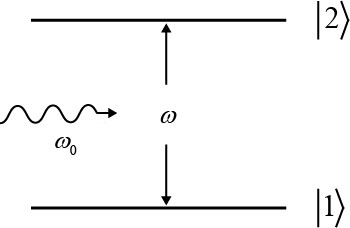
\includegraphics[scale=0.5]{Img/Fig_1.jpg}
	\bicaption{经典场与二能级原子相互作用示意图}{Schematic diagram of interaction between classical field and two-level atom}	\label{figure}
\end{figure}

如图\ref{figure}中,我们用$\ket{1}$和$\ket{2}$表示二能级原子的基态和激发态,能量本征值分别为$\hbar \omega_1$和$\hbar \omega_2$,经典场的频率为$\omega_0$。一个单模场与这个系统发生相互作用,描述系统的哈密顿量为
\begin{align}
H = {H_0} + {H_I} = \hbar {\omega _1}\left| 1 \right\rangle \left\langle 1 \right| + \hbar {\omega _2}\left| 2 \right\rangle \left\langle 2 \right| - er \cdot E(\bm
{r},t),\label{eq43}
\end{align}
其中
\begin{align}
{H_0} = \hbar {\omega _1}\left| 1 \right\rangle \left\langle 1 \right| + \hbar {\omega _2}\left| 2 \right\rangle \left\langle 2 \right|,\label{eq44}
\end{align}
为原子的自由哈密顿量。相互作用哈密顿量为
\begin{align}\label{eq45}
\begin{split}
{H_I} &=  - e\bm{r} \cdot E(t)\\
      &= - e\left( {\left| 1 \right\rangle \left\langle 1 \right| + \left| 2 \right\rangle \left\langle 2 \right|} \right) \cdot \bm{r} \cdot \left( {\left| 1 \right\rangle \left\langle 1 \right| + \left| 2 \right\rangle \left\langle 2 \right|} \right)E\left( t \right)\\
      &=  - e\left( {{u_{12}}{\sigma _{12}} + {u_{21}}{\sigma _{21}}} \right)E\left( t \right)
\end{split}
\end{align}
上面我们用到了关系式$\sum_i\sigma_{ii}=1$,$\sigma_{ij}=\ket{j}\bra{j}$是原子算符,$u_{12}=u_{21}^*=e\bra{1}r\ket{2}$是跃迁偶极矩阵元。假设电场沿着$r$方向极化,在偶极近似的条件下,电场可表示为
\begin{align}
E(t) = {E_0}\cos (vt) = \frac{1}{2}{E_0}({e^{i{\omega _0}}} + {e^{ - i{\omega _0}t}}),\label{eq46}
\end{align}
为了方便表述,我们定义场的拉比频率
\begin{align}
\Omega  = \frac{{{u_{21}}{E_0}}}{{2\hbar }},\label{eq47}
\end{align}
于是相互作用的哈密顿量可以写为
\begin{align}
{H_I} =  - \hbar \left( {{\Omega ^*}{\sigma _{12}} + \Omega {\sigma _{21}}} \right)({e^{i{\omega _0}}} + {e^{ - i{\omega _0}t}}),\label{eq48}
\end{align}
在相互作用绘景下,通过对相互作用哈密顿量做幺正变换,我们得到
\begin{align}\label{eq49}
\begin{split}
{V_I} =& {e^{i{H_0}t}}{H_I}{e^{ - i{H_0}t}}\\
      =&  - \hbar \Omega {\sigma _{21}}{e^{i\left( {\omega  - {\omega _0}} \right)t}} - \hbar {\Omega ^*}{\sigma _{12}}{e^{ - i\left( {\omega  - {\omega _0}} \right)t}}\\
&- \hbar \Omega {\sigma _{21}}{e^{i\left( {\omega  + {\omega _0}} \right)t}} - \hbar {\Omega ^*}{\sigma _{12}}{e^{ - i\left( {\omega  + {\omega _0}} \right)t}},
\end{split}
\end{align}
其中$\omega=\omega_2-\omega_1$。在上式中我们采用旋转波近似,略去两个快速振荡的项之后,系统的哈密顿量最终可以变为如下的形式
\begin{align}
{V_I} =  - \hbar \Omega {\sigma _{21}}{e^{i\left( {\omega  - {\omega _0}} \right)t}} - \hbar {\Omega ^*}{\sigma _{12}}{e^{ - i\left( {\omega  - {\omega _0}} \right)t}}.\label{eq50}
\end{align}

\subsection{单模光场与二能级原子相互作用的全量子描述}\label{paf}

\begin{figure}[htbp]
	\centering
	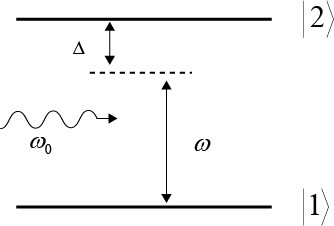
\includegraphics[scale=0.5]{Img/Fig_2.jpg}
	\bicaption{单模光场与二能级原子相互作用示意图}{Schematic diagram of interaction between single-model field and two-level atom}	\label{figure2}
\end{figure}

全量子描述就是将光场和原子都做了量子化处理。单模场与单个二能级原子的相互作用是量子光场与物质相互作用的最简单模型,称为拉比模型,取旋转波近似后的形式称为Jaynes-Cummings模型(简称J-C模型)。

如图\ref{figure2}所示,原子的自由哈密顿量为
\begin{align}
{H_A} = \hbar {\omega _1}\left| 1 \right\rangle \left\langle 1 \right| + \hbar {\omega _2}\left| 2 \right\rangle \left\langle 2 \right|,\label{eq51}
\end{align}
选取能量零点使得$\hbar {\omega _2}{\rm{ = }}\frac{1}{2}\hbar \omega$,$\hbar {\omega _1}{\rm{ = }} - \frac{1}{2}\hbar \omega$, $\omega  = {\omega _2} - {\omega _1}$,并引入泡利算符${\sigma _z} = \left| 2 \right\rangle \left\langle 2 \right| - \left| 1 \right\rangle \left\langle 1 \right|$,则有
\begin{align}
{H_A} = \frac{1}{2}\hbar {\omega _0}{\sigma _z},\label{eq52}
\end{align}

单模光场的自由哈密顿量为
\begin{align}
{H_F} = \hbar {\omega _0}{a^\dag }a,\label{eq53}
\end{align}
上式中略去了与光场自由哈密顿量无关紧要的常数项$\hbar \omega/2$。

相互作用的哈密顿量为
\begin{align}\label{eq54}
\begin{split}
{H_I} &= \sum\limits_{j,k} {\sum\limits_\lambda  {\hbar {g_{jk,\lambda }}} } \left| j \right\rangle \left\langle k \right|({a_\lambda } + a_\lambda ^\dag )\\
&= \sum\limits_{j,k} {\hbar {g_{jk}}\left| j \right\rangle \left\langle k \right|(a + {a^\dag })} \\
&= \left( {\hbar {g_{21}}\left| 2 \right\rangle \left\langle 1 \right| + \hbar {g_{12}}\left| 1 \right\rangle \left\langle 2 \right|} \right)(a + {a^\dag })\\
&= \hbar \lambda \left( {\left| 2 \right\rangle \left\langle 1 \right| + \left| 1 \right\rangle \left\langle 2 \right|} \right)(a + {a^\dag })\\
&= \hbar \lambda \left( {{\sigma ^{\rm{ + }}} + {\sigma ^ - }} \right)(a + {a^\dag }),
\end{split}
\end{align}
其中${\sigma ^ + }{\rm{ = }}\left| 2 \right\rangle \left\langle 1 \right|$,${\sigma ^ - } = \left| 1 \right\rangle \left\langle 2 \right|$,并假设$g_{21}=g_{12}=\lambda$。

于是可得,系统的总的哈密顿量为
\begin{align}\label{eq55}
\begin{split}
H &= {H_A} + {H_F} + {H_I}\\
&= \frac{1}{2}\hbar {\omega _0}{\sigma _z} + \hbar {\omega _0}{a^\dag }a + \hbar \lambda \left( {{\sigma ^ + } + {\sigma ^ - }} \right)(a + {a^\dag }),
\end{split}
\end{align}
上式中,相互作用哈密顿量中四项的物理意义分别为:$\sigma^+a$表示原子吸收一个光子从低能级跃迁到高能级;$\sigma^-a^\dagger$表示原子从高能级跃迁到低能级并放出一个光子;$\sigma^-a$表示原子从高能级跃迁到低能级的同时吸收一个光子;$\sigma^+a^\dagger$表示原子从低能级跃迁到高能级的同时放出一个光子。

在旋转波近似下,略去方程(\ref{eq55})中能量不守恒的项以后,系统的哈密顿量变为
\begin{align}
H = \frac{1}{2}\hbar {\omega _0}{\sigma _z} + \hbar {\omega _0}{a^\dag }a + \hbar \lambda \left( {{\sigma ^ + }a + {\sigma ^ - }{a^\dag }} \right),\label{eq56}
\end{align}
将上式变换到相互作用绘景,可得相互作用绘景中的相互作用哈密顿量为
\begin{align}
{H_I} = \hbar \lambda \left( {{\sigma ^ + }a{e^{i\Delta t}} + {a^\dag }{\sigma ^ - }{e^{ - i\Delta t}}} \right),\label{eq57}
\end{align}
其中$\omega-\omega_0$为原子和场的失谐量。

J-C模型虽然是在基于电偶极近似与旋转波近似的前提下推导出来的,但是由于J-C模型是可积的,即可以得到精确解析的结果,所以它的重要性不言而喻,而正因为如此,所以它也成为了在量子光学中研究问题的一个最基本的模型。
而它之所以重要并不仅在于其模型可精确求解的缘故,更在于它预测了一系列的实验结果,比如拉比震荡(Rabi oscillating)\cite{rabi1937space,cummings2013reminiscing},原子布居数的坍塌-复苏\cite{rempe1987observation,eberly1980periodic},真空中的自发辐射过程,光子反聚束\cite{haroche2013nobel,wineland2013nobel},纠缠\cite{rauschenbeutel2000step,phoenix1991establishment}以及亚迫松分布等。

















\vbox{}
\section{自旋压缩态}
\vbox{}
压缩态概念最早的出现是在光学中,由于压缩态很多非经典态所没有的特性,因此对压缩态的研究显得格外重要。由于压缩光在光学高精度测量中可以降低光子计数噪声、提高非破坏性%(quantum nondemolition, QND)
测量的灵敏度和光通信等方面有着重要的应用,所以被引入到自旋系统,称之为自旋压缩态。自旋压缩态与光的压缩态相比在存储和保真度方面更容易实现,而且在量子信息的研究方面扮演着很重要的角色,故而关于自旋压缩态的研究受到了广泛的关注。

本节内容主要介绍了一些关于自旋压缩态的一些概念,包括光场压缩态的相关知识、自旋压缩态的基本概念、定义和压缩参数等内容。

\subsection{光场的压缩态}\label{section31}

压缩态的概念最先存在于光学中,最初由David Stole提出,在上个世纪七八十年代开始压缩光由于在引力波测量、精密测量以及光通信等方面的重要应用而受到重视。

光场的湮灭算符$a$和产生算符$a^\dagger$可按实部与虚部展开:
\begin{align}
	a = {X_1} + i{X_2},{a^\dag } = {X_1} - i{X_2},\label{eq331}
\end{align} 
由于$a$和$a^\dagger$之间的对易关系满足
\begin{align}
	\left[ {a,{a^\dag }} \right] = 1,\label{eq332}
\end{align}
因此可以得到
\begin{align}
	\left[ {{X_1},{X_2}} \right] = i/2,\label{eq333}
\end{align}
引入$A,B$两个算符,根据海森堡不确定度关系我们可以得到
\begin{align}\label{eq334}
	V\left( A \right)V\left( B \right) \ge \frac{1}{4}{\left| {\left\langle {\left[ {A,B} \right]} \right\rangle } \right|^2},
\end{align}
于是有
\begin{align}\label{eq335}
	V\left( {{X_1}} \right)V\left( {{X_2}} \right) \ge \frac{1}{{16}},
\end{align}
其中,$V\left( {{X_i}} \right)\left( {i = 1,2} \right)$为正交分量$X_i$的方差。

引入标准偏差$\Delta A \equiv \sqrt {V\left( A \right)} $,则式(\ref{eq334})和式(\ref{eq335})又可表示为
\begin{align}
	&( \Delta A)(\Delta B) \ge \frac{|\braket{[A,B]}|^2}2,\label{eq336}\\
	&( \Delta X_1)( \Delta X_2) \ge 1/4,\label{eq337}
\end{align}
在公式(\ref{eq337})中取等号的态我们将其称之为最小的不确定度态,即相干自旋态%(coherent spin state, CSS)
。当$\Delta X_1^2\left( {\Delta X_2^2} \right) < 1/4$时,如果有$\Delta X_2^2\left( {\Delta X_1^2} \right) >1/4$,而此时海森堡不确定度关系依旧成立,我们可以看到其中有一个不确定度已经小于相干态的量子涨落所能达到的最小值(1/4),产生了压缩现象,因此我们就称此时光场处于压缩态。这就是光场压缩态的定义。

\subsection{自旋压缩的定义}

在研究自旋压缩的过程中,自旋压缩的定义并不是唯一的,它取决于具体研究的系统,目前被广泛接受的定义是由Kitagawa和Ueda类似于光的压缩态提出的定义\cite{PRA1993Kitagawa},以及Wineland等人\cite{PRA1994Wineland}在研究Ramsey实验时提出的定义。除了这两个被广泛研究的定义之外,还有一些其他的自旋压缩定义\cite{sorensen2001many,toth2009spin,wang2010sudden}被提出,这些定义是为了某些考虑而引入的。

受到光场的压缩态启发,类比于光场的压缩,K. W\'odkliewicz和Eberly\cite{wodkiewicz1987k}这么定义了自旋压缩态:
将自旋算符$\mathbf{S}$在三维的直角坐标轴上正交分解为$S_x$,$S_y$和$S_z$,它们之间满足对易关系
\begin{align}
	\left[ {{S_x},{S_y}} \right] = i{S_z}\left( {\hbar  = 1} \right),\label{eq338}
\end{align}
此时,根据海森堡不确定度关系我们将得到
\begin{align}
	{\left( {\Delta {S_x}} \right)^2}{\left( {\Delta {S_y}} \right)^2} \ge \frac{{{{\left| {\left\langle {{S_z}} \right\rangle } \right|}^2}}}{4},\label{eq339}
\end{align}
当$(\Delta S_x)^2=(\Delta S_y)^2=\braket{ S_z}/2$时,系统就处于相干态。如果$(\Delta S_i)^2<\braket{S_z}/2$$(i=x,y)$,则系统此时处于自旋压缩态。

这个看似合理的定义实际上是不具完备性的,因为它仅仅只是通了过坐标系的旋转就将相干自旋态变成了自旋压缩态,这显然是不正确的。在证明这个定义不正确之前,我们先来证明一下相干态的实质是所有的自旋都沿着同一个方向极化的态。我们这里假设所有的方向都指向$z$轴的正方向,则系统所处的态可以表示为$\ket{S,S}$,我们在这个态下计算各个原子自旋分量的平均值及平方的平均值我们将得到如下的结果:
\begin{align}\label{eq3310}
	\begin{split}
		\braket{S_x}    &= \braket{S_y}  = 0,	\braket{S_z}  = S,\\
		\braket{S_x^2}  &= \bra{S,S}(\frac{S_++S_-}2)^2\ket{S,S} \\
		            	&= \bra{S,S}S_+S_-\ket{S,S}/4\\
		            	&= S/2,\\
		\braket{S_y^2}  &= \bra{S,S}(\frac{S_+-S_-}{2i})^2\ket{S,S} \\
		            	&= \bra{S,S}S_+S_-\ket{S,S}/4\\
			            &= S/2,\\
		(\Delta S_x)^2  &= (\Delta S_y)^2 = \braket{S_z}/2,
	\end{split}
\end{align}
现在我们将证明这个定义为什么不正确。假设一个系统最初处于相干态,平均自旋指向$z$轴正方向(如图\ref{figure3}所示),即$\braket{S}=\braket{S_z}$,则有$(\Delta S_x)^2  = (\Delta S_y)^2 = \braket{S_z}/2$,如果将$y$-$z$平面绕着$x$轴旋转一个角度$\theta$,$y$,$z$到达新的位置$y'$,$z'$。
\begin{figure}[h!]
	\centering
	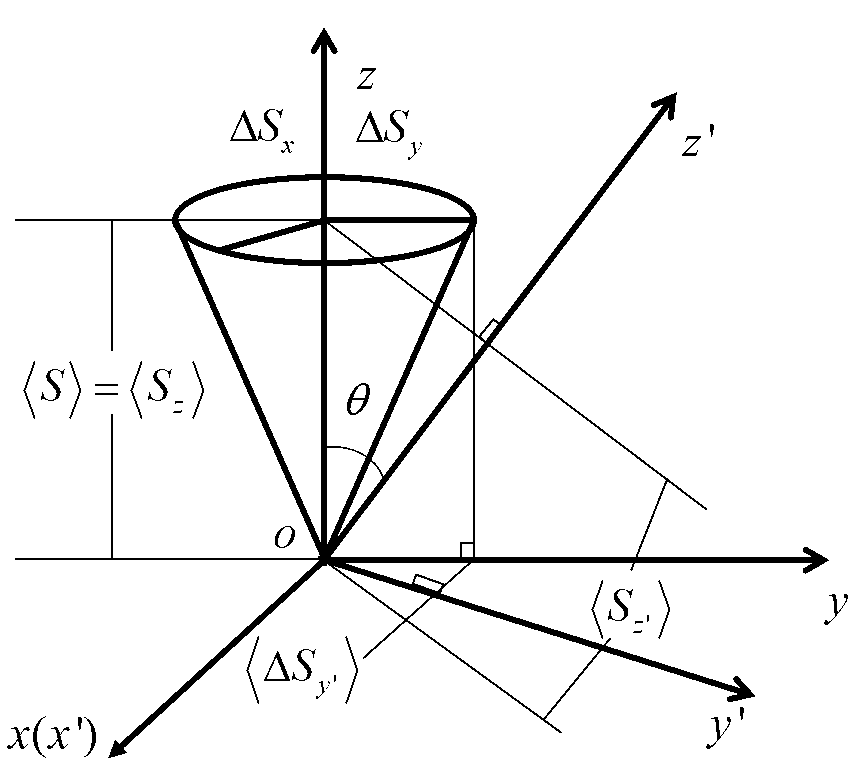
\includegraphics[scale=0.45]{Img/Fig_3.png}\\
	\vspace{0.5cm}
	\bicaption{角动量及其变化量在不同坐标系中的投影}{Projection of angular momentum and its variation in different coordinate systems}	\label{figure3}
\end{figure}

在新的坐标系中,因为:
\begin{align}\label{eq3312}
	\begin{split}
		\Delta S_{x'} & = \Delta {S_x}\\
		\braket{S_{z'}} & = \braket{S_{z'}}  \cos \theta \\
		\Delta {S_{y'}} & = \Delta {S_y}\cos \theta ,
	\end{split}
\end{align}
所以有
\begin{align}\label{eq3313}
	\begin{split}
		\Delta S_{x'}^2 &= \frac{\braket{S_z}}{2} \ge \frac{\braket{S_{z'}}}{2}\\
		\Delta S_{y'}^2 &= \Delta S_y^2~{\cos ^2}\theta  \le \frac{\braket{S_z}}{2}\cos \theta  = \frac{\braket{S_{z'}}}{2},
	\end{split}
\end{align}
如果$\theta\ne 0$,$\Delta S_{x'}^2 > \braket{S_{z'}}/2$,$\Delta S_{y'}^2 < \braket{S_{z'}}/2$。根据上述自旋压缩的定义,在$x'y'z'$坐标系中系统现在处于压缩态。

上述的证明表明在这样的定义下,仅仅只是通过旋转了坐标系,系统便由原来的相干态转化成压缩态,这显然是不正确的,因为通过旋转坐标并没有对系统进行任何操作,系统没有发生任何变化。而且,旋转坐标只是通过哈密顿量的线性作用,而光压缩的产生需要非线性哈密顿量的作用才可以产生,因此这个定义显然是不合理的。

在这个基础上Kitagawa和Ueda提出了更加普遍的定义,他们认为,考察的对象应该是垂直于总自旋方向的自旋分量,如果这个分量的最小不确定量的平方小于相干态所能达到的最小值,则系统便是处于自旋压缩态。为了计算方便,在选择坐标时一要尽量使系统的平均总自旋处于直角坐标轴上。

\subsection{自旋压缩的数学表示}

考虑由$N$个1/2自旋的原子组成的系综,这个自旋1/2原子系综的角动量算符由下式给出
\begin{align}
	{J_\alpha } = \frac{1}{2}\sum\limits_{l = 1}^N {{\sigma _{l\alpha }}} ,\alpha  = x,y,z,\label{eq3314}
\end{align}
其中$\sigma_{l\alpha}$是第$l$个原子的泡利矩阵。在讨论自旋压缩态之前,先介绍一下相干自旋态(Coherent spin state, CSS)。

CSS可以写成单个自旋态的直积形式
\begin{align}
	\left| {\theta ,\phi } \right\rangle  = \mathop  \otimes \limits_{l = 1}^N \left[ {\cos \frac{\theta }{2}{{\left| 0 \right\rangle }_l} + {e^{i\phi }}\sin \frac{\theta }{2}{{\left| 1 \right\rangle }_l}} \right],\label{eq3315}
\end{align}
其中$\ket{0}_l$和$\ket{1}_l$表示算符$\sigma_{lz}$的本征值分别为1和-1的本征态,在上式的定义中,所有的自旋都指向同一个方向。利用下式
\begin{align}
	\exp \left[ {i\left( {\xi {\sigma _ + } + \eta {\sigma _ - }} \right)} \right] = \cos \sqrt {\xi \eta }  + i\frac{{\sin \sqrt {\xi \eta } }}{{\sqrt {\xi \eta } }}\left( {\xi {\sigma _ + } + \eta {\sigma _ - }} \right),\label{eq3316}
\end{align}
可以将CSS写成如下的形式
\begin{align}
	\left| {\theta ,\phi } \right\rangle  = \mathop  \otimes \limits_{l = 1}^N {R_l}\left( {\theta ,\phi } \right){\left| 0 \right\rangle _l} = \mathop  \otimes \limits_{l = 1}^N \exp \left( {\varsigma {\sigma _ + } - {\varsigma ^*}{\sigma _ - }} \right){\left| 0 \right\rangle _l},\label{eq3317}
\end{align}
其中
\begin{align}
	\varsigma  =  - \frac{\theta }{2}\exp \left( {i\phi } \right),\label{eq3318}
\end{align}
更进一步地可以将CSS表示为
\begin{align}
	\ket {\theta ,\phi }  = {R_l}(\theta ,\phi )\ket {j,j}= \exp ( {\varsigma {J_ + } - {\varsigma ^*}{J_ - }} )\ket {j,j}  ,\label{eq3319}
\end{align}
其中
\begin{align}
	\left| {j,j} \right\rangle  \equiv \mathop  \otimes \limits_{l = 1}^N {\left| 0 \right\rangle _l},\label{eq3320}
\end{align}
$\ket{j,j}$表示算符$J_z$本征值为$j=N/2$的本征态,这就意味着所有的自旋分量都在$z$轴方向上。其中
\begin{align}
	{J_ \pm } = {J_x} \pm i{J_y},\label{eq3321}
\end{align}
为跃迁算符,$R\left( {\theta ,\phi } \right)$为旋转算符,由下面的式子给出
\begin{align}
	R\left( {\theta ,\phi } \right) = \exp \left( { - i\theta {J_{\vec n}}} \right) = \exp \left[ { - i\theta \left( {{J_x}\sin \phi  - {J_y}\cos \phi } \right)} \right],\label{eq3322}
\end{align}
其中$\vec n = \left( { - \sin \phi ,\cos \phi ,0} \right)$。

角动量算符的对易关系
\begin{align}
	\left[ {{J_\alpha},{J_\beta}} \right] = i{\varepsilon _{\alpha\beta\gamma}}{J_\gamma},\label{eq3323}
\end{align}
其中$\alpha,\beta,\gamma$表示任意三个正交方向的分量。$\varepsilon _{\alpha\beta\gamma}$是Levi-Civita符号。不确定关系是
\begin{align}
(\Delta J_\alpha)^2(\Delta J_\beta)^2\ge |\braket{ J_\gamma}|^2/4,\label{eq3324}
\end{align}
当上式左边的两个涨落中有一个满足
\begin{align}\label{eq3325}
	\begin{split}
	(\Delta J_\beta)^2\le |\braket{ J_\gamma}|/2,
	\end{split}
\end{align}
我们就说这个系统是被压缩的。也就是说,由于原子之间非经典关联的缘故\cite{PRA1993Kitagawa},在不违法海森堡不确定度关系的前提下,两个正交分量的不确定度被重新分配,其中一个角动量分量的不确定度将小于标准量子极限。这种自旋角动量在某个方向的涨落减小的态称为自旋压缩态。

对于一个原子系统,如果各个原子之间未能产生量子关联,则其各个原子的自旋分量的方向应该沿空间各方向平均自由分布,在垂直于平均自旋的平面内的任意相互垂直的两个方向上都分布着相同的总自旋,没有压缩性质的存在,如图(a)所示的自旋角动量。如果自旋角动量的涨落在某一方向上部分地减小,则表明在各个自旋单体之间建立起某种关联,正是这种量子关联效应导致了自旋压缩,如图(b)所示,而这种压缩同时也导致了其垂直方向上涨落的增加,压缩的增加与海森堡不确定关系仍旧成立,这是自旋压缩的基本原理。我们也可以把处于自旋压缩态的自旋矢量设想成一个椭圆形圆锥,如图\ref{figure4}所示。
\begin{figure}[htbp]
	\centering
	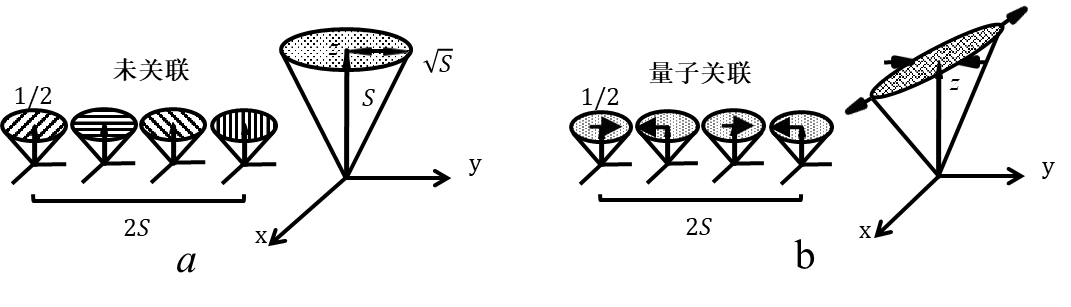
\includegraphics[scale=0.78]{Img/Fig_4.png}
	\bicaption{
		2S个独立的自旋1/2原子的S个自旋态的示意图。
		(a) 2S个未关联的1/2自旋构成的相干自旋态。
		(b) 2S个关联的1/2自旋构成的自旋压缩态。}
	{Schematic illustrations of S-spin states in terms of 2S individual 1/2 spins. 
		(a) Coherent spin state constructed from 2S uncorrelated 1/2.
		(b) Squeezed spin state constructed from 2S correlated 1/2.
	}	
	\label{figure4}
\end{figure}


\subsection{自旋压缩参数}

对于一个特定的系统而言,其自旋压缩一般是利用自旋压缩系数来进行判定的。关于自旋压缩系数的定义,相关文献\cite{MA201189}中论及的有好几种,但究竟哪一种是最好的到目前都还没有定论。比较典型的是Kitagawa和Ueda给出的定义以及Wineland等人给出的定义。下面我们分别来看一下这两种定义。

Kitagawa和Ueda给出的定义:
\begin{align}
	\xi _K^2 = \frac{{2\min {{\left( {\Delta {J_{{{\vec n}_ \bot }}}} \right)}^2}}}{j} = \frac{{4\min {{\left( {\Delta {J_{{{\vec n}_ \bot }}}} \right)}^2}}}{N},\label{eq3326}
\end{align}

Wineland等人给出的定义:
\begin{align}
	\xi _W^2 = \frac{{N{{\left( {\Delta {J_{{{\vec n}_ \bot }}}} \right)}^2}}}{{{{\left| {\left\langle {{J_{{{\vec n}_ \bot }}}} \right\rangle } \right|}^2}}},\label{eq3327}
\end{align}
在上式中,下标${\vec n_ \bot }$指的是与平均自旋方向$\vec n=\braket{J}/\sqrt{\braket{J}\braket{J}}$垂直的方向。对于相干自旋态,我们有$(\Delta {J_{{\vec n}_ \bot} })^2=j/2$,如果$J_{{\vec n}_ \bot} $小于$j/2$,则此时处于自旋压缩态。 ${J_{{{\vec n}_ \bot }}}=J \cdot {\vec n_ \bot }$可以利用方差${\left( {\Delta J} \right)^2}$的最小值来计算自旋压缩系数。如果上述表达式$\xi _K^2 \le 1\left( {\xi _W^2 \le 1} \right)$,则系统是自旋压缩的。$\xi _K^2 \le 1\left( {\xi _W^2 \le 1} \right)$的值越小,自旋压缩发生的程度越大。

我们先介绍Kitagawa和Ueda的定义,在式(\ref{eq3326})中$\min {\left( {\Delta {J_{{{\vec n}_ \bot }}}} \right)^2}$指垂直于平均自旋方向投影与垂直平面上的最小自旋不确定度。若给定了平均自旋角动量的方向
\begin{align}
	{\vec n_0} = \left( {\sin \theta \cos \phi ,\sin \theta \sin \phi ,\cos \theta } \right),\label{eq3328}
\end{align}
其中极化角和方位角分别为
\begin{align}\label{eq3329}
	\left\{ \begin{array}{ll}
		\theta&=\arccos (\braket{J_z}/|J|)\\
		\phi &= 2\pi + (\braket{J_y}/|\braket{J_y}|)\arccos (\braket{J_x}/|J\sin \theta|),
	\end{array} \right.
\end{align}
则垂直${\vec n_0}$的平面内的两个相互垂直的矢量为
\begin{align}\label{eq3330}
	\left\{ \begin{array}{ll}
		{\vec n_1} &= (-\sin\varphi, \cos\phi,0)\\
		{\vec n_2} &= (\cos\theta\cos\varphi, \cos\theta\sin\varphi, -\sin\varphi),
	\end{array} \right.
\end{align}
即满足${\vec n_0} \cdot {\vec n_1} = {\vec n_0} \cdot {\vec n_2} = {\vec n_1} \cdot {\vec n_2} = 0$,因此,在垂直于平均自旋角动量方向的平面内的任意自旋角动量方向总可以表示成
\begin{align}
	{\vec n_ \bot } = {\vec n_1}\cos \phi  + {\vec n_2}\sin \phi ,\label{eq3331}
\end{align}
于是,系统总的角动量在某矢量的投影可以表示为
\begin{align}
	{J_{{{\vec n}_ \bot }}} = J \cdot {\vec n_ \bot } = J \cdot {\vec n_1}\cos \phi  + J \cdot {\vec n_2}\sin \phi  = {J_{{n_1}}}\cos \phi  + {J_{{n_2}}}\sin \phi ,\label{eq3332}
\end{align}
将式(\ref{eq3326})带入$\Delta J_{{{\vec n}_ \bot }}^2$后,通过计算可得
\begin{align}\label{eq3333}
	\begin{split}
		\xi _K^2 &= \frac{2}{N}\min \left[ \braket{J_{n_1}^2 + J_{n_2}^2}+ \cos (2\theta)\braket{J_{n_1}^2 - J_{n_2}^2}\right] + \sin ( 2\theta )
		\braket{\left[ J_{n_1},J_{n_2} \right]_+ }^2\\
		&= \frac{2}{N}\left[\braket{J_{n_1}^2 + J_{n_2}^2}- \sqrt {\braket{J_{n_1}^2 - J_{n_2}^2} + \braket{\left[ J_{n_1},J_{n_2} \right]_+ }^2} \right],
	\end{split}
\end{align}



现在我们讨论Wineland等人提出的自旋压缩参数。在Ramsey光谱学的研究中。压缩参数ξR2是在Ramsey光谱中确定共振频率时一般状态和CSS之间的波动的比率。这里的CSS充当噪声参考状态。与ξS2相比,ξS2是玻色子压缩的类比,参数ξR2基本上与角动量状态对旋转的灵敏度的改善相关,因此对于实验是有吸引力的。




Wineland等人提出的定义是在研究Ramsey光谱学的时候提出来的,压缩参数$\xi_W$是在Ramsey光谱中确定共振频率时一般状态和CSS之间的涨落的比率。在实验中如果初态刚开始处于CSS,则相位不确定度为${\left( {\Delta \phi } \right)_{CSS}} = {1 / {\sqrt N }}$,把它称为标准量子极限。如果相位不确定度满足${\left( {\Delta \phi } \right)_{CSS}} <{1 / {\sqrt N }}$,我们就称其处于自旋压缩态。他们的定义为
\begin{align}
	\xi _W^2 = \frac{{{{\left( {\Delta \phi } \right)}^2}}}{{\left( {\Delta \phi } \right)_{CSS}^2}} = \frac{{N\left( {\Delta {J_{{n_ \bot }}}} \right)}}{{{{\left| {\left\langle J \right\rangle } \right|}^2}}},\label{eq3334}
\end{align}
一般情况下,$|\braket{J}| \le  N/2$,因此	
\begin{align}
	\xi _W^2 = \frac{{N\left( {\Delta {J_{{n_ \bot }}}} \right)}}{{{{\left| {\left\langle J \right\rangle } \right|}^2}}} \ge \frac{{N\left( {\Delta {J_{{n_ \bot }}}} \right)}}{N} = \xi _K^2,\label{eq3335}
\end{align}
我们可以看出来Kitagawa和Ueda的自旋压缩参数是从海森堡不确定关系出发的,考虑的是垂直于自旋方向的涨落和$J/2$的关系。而Wineland等人的定义则是从测量和参数估计出发,利用自旋压缩参数来看能突破标准量子极限的程度的。具体选用哪一种参数和具体研究的体系和问题有关系,这是目前使用最多的两种定义,除此之外还有一些其它的定义,祥见参考文献\cite{MA201189}。
\subsection{自旋压缩的产生}	

目前产生自旋压缩态的方法已经有很多种,但是大致可以归纳以下两类:

(1) 在原子系综中通过光与原子的相互作用产生自旋压缩态。非常自然的一个想法就是将光的压缩态转移到自旋系统,许多方案中也提到通过电磁感应透明来转移压缩。当考虑光原子相互作用时,光与原子之间的失谐是非常重要的。在大失谐的情况下,可以得到系统有效的哈密顿量,包括色散相互作用项和非线性相互作用项,并且可以调整这两个项的大小。  
  (a)光与原子之间的色散相互作用导致光的偏振的法拉第旋转。然后通过对输出光进行量子非破坏性(quantum nondemolition, QND)测量,可以将原子系综在测量结果的条件下压缩,该方法已经在实验中实现。  
  (b)描述原子间相互作用的非线性项是单轴扭曲哈密顿量,可用于产生自旋压缩。

(2) 在玻色-爱因斯坦凝聚(Bose–Einstein condensations, BEC)中通过原子之间的碰撞来产生自旋压缩态。
在过去十年中,在BEC中产生自旋压缩状态引起了相当大的兴趣。双组分BEC中的非线性原子-原子碰撞可以用单轴扭曲哈密顿量来描述,它通常用于产生自旋压缩态。此外,双轴扭转哈密顿量可以通过拉曼过程实现,也可以通过双阱势中的双组分冷凝物来实现。自旋压缩也可以通过自旋交换相互作用或自由动力学演化在自旋-1 BEC中产生。

自旋压缩产生的关键是在粒子之间产生相互关联,这种关联可以通过粒子之间的非线性相互作用来实现。在文献\cite{PRA1993Kitagawa}中,Kitagawa和Ueda不仅重新定义了自旋压缩态,与此同时还提出了两种用于产生自旋压缩非线性哈密顿量的模型:单轴扭曲模型(One-axis twisting Hamiltonian)和双轴扭曲模型的哈密顿量(two-axis twisting Hamiltonian)。接下来我们简单介绍一下这两种模型。

\subsubsection{单轴扭曲模型}

在基础自旋之间建立量子关联,需要非线性的相互作用。现在考虑一个由哈密顿量$H=\hbar F(S_z)$生成的幺正算符为$U(t)=exp[-itF(S_z)]$,通过这个幺正算符我们可以写出它的升降算符为${S_ \pm } \equiv {S_x} \pm i{S_y}$,其演化方式可以表述为如下的形式
\begin{align}
	{S_ + }\left( t \right) = {U^\dag }{S_ + }\left( 0 \right)U = {S_ + }\left( 0 \right)\exp \left[ {itf\left( {{S_z}} \right)} \right],\label{eq3336}
\end{align}
和${S_-}\left( t \right) = {\left[ {{S_ + }\left( t \right)} \right]^\dag }$,其中
\begin{align}
	f\left( {{S_z}} \right) = F\left( {{S_z}{\rm{ + }}1} \right) - F\left( {{S_z}} \right),\label{eq3337}
\end{align}
对于最低次幂的非线性相互作用$F(S_z)=\chi S_z^2$将导致$f(S_z) = 2\chi (S_z+1/2)$,即与$S_z$成比例的旋转,将量子涨落进行扭转。
扭转之后的角动量算符的$x$分量和$y$分量分别为${S_x}(t)= \frac12(S_+e^{i\mu(S_z+1/2)}+e^{-i\mu(S_z+1/2)}S_z)$和${S_y}(t)= \frac{1}{2i}(S_+e^{i\mu(S_z+1/2)}-e^{-i\mu(S_z+1/2)}S_z)$,其中$\mu  \equiv 2\chi t$。不确定度在$y-z$平面的正交分量上发生了重新分布,如图\ref{figure5}所示。
\begin{figure}[h!]
	\centering
	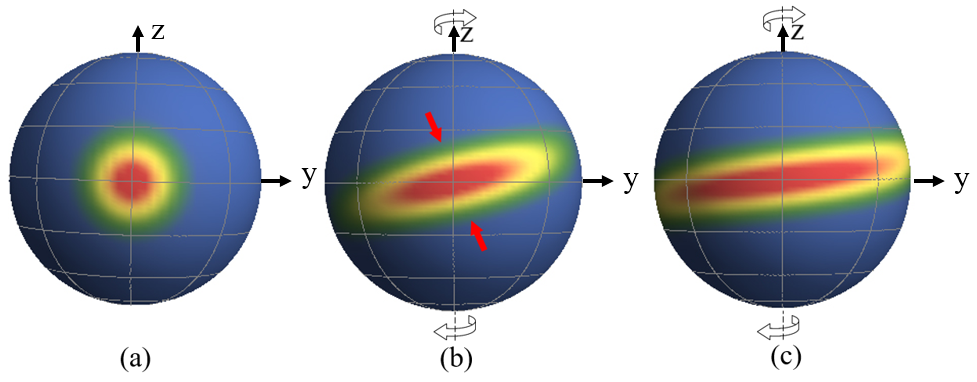
\includegraphics[scale=0.42]{Img/oat2.png}
	\bicaption{当S=20时,准概率分布(quasi-probability distribution, QPD)表示出的单轴扭曲模型所引起的态演化。图中的密度通过$Q(\theta,\phi)$最大值$Q_{max}$进行了归一化。(a)显示初始相干自旋态$\ket{\theta=\pi/2,\phi=0}(Q_{max}=1)$。(b)和(c)显示由$U=exp[-i\mu S_z^2/2]$产生的单轴扭曲模型的态; (b)最优压缩出现在$\mu=0.199(Q_{max}=0.445)$; (c)显示在$\mu=0.399(Q_{max}=0.241)$的过度扭曲。(c)中的QPD与测地线有所偏移。}
	{State evolutions by one-axis twisting in terms of the quasiprobability distribution (QPD) on the sphere for S = 20. The densities of the figures are normalized by the maximum value $Q_{max}$ of $Q(\theta,\psi)$. (a) shows the initial coherent spin state $\ket{\theta=\pi/2,\phi=0}(Q_{max}=1)$. (b) and (c) show one-axis twisted states generated by the unitary transformation $U=exp[-i\mu S_z^2/2]$; (b) optimally squeezed at $\mu=0.199(Q_{max}=0.445)$ and (c) excessively twisted at $\mu=0.399(Q_{max}=0.241)$. Although not clear from the figure, the QPD of (c) deviates from a geodesic (swirliness).}
	\label{figure5}
\end{figure}
\subsubsection{双轴扭曲模型}

虽然OAT模型可以有效地产生自旋压缩,但其最佳压缩角度却与系统的尺寸和演化时间有着密切的关系。如果在垂直于平均自旋方向的平面中围绕两个正交轴顺时针和逆时针同时进行扭转,则可以完美的解决这个问题。如图\ref{figure6}所示,若初始态CSS$\ket{0,\phi}$沿$\theta=\pi/2$,$\phi=\pm \pi/4$两个轴进行反向扭转,双轴反向扭曲的哈密顿量可以写成
\begin{align}
	H  = \chi(S_{\pi/2,\pi/4}^2-S_{\pi/2,-\pi/4}^2)
	= \frac{\chi}{2i}(S_+^2-S_-^2),\label{eq3338}
\end{align}
在参考文献\cite{helmerson2001creating,zhang2003entanglement,wesenberg2002mixed}提出了几种如何产生这个哈密顿量的方法。

当S较小时,双轴扭曲的自旋压缩态可以达到的最小方差小于1/2,随着S增大,最小方差趋近于1/2。当被压缩的方差达到1/2时,增强方差可以达到$S^2/2$。当$S^2/2$超过最优值时,QPD分成两个部分。双轴反向扭曲可以最大化地消除噪音。
\begin{figure}[h!]
	\centering
	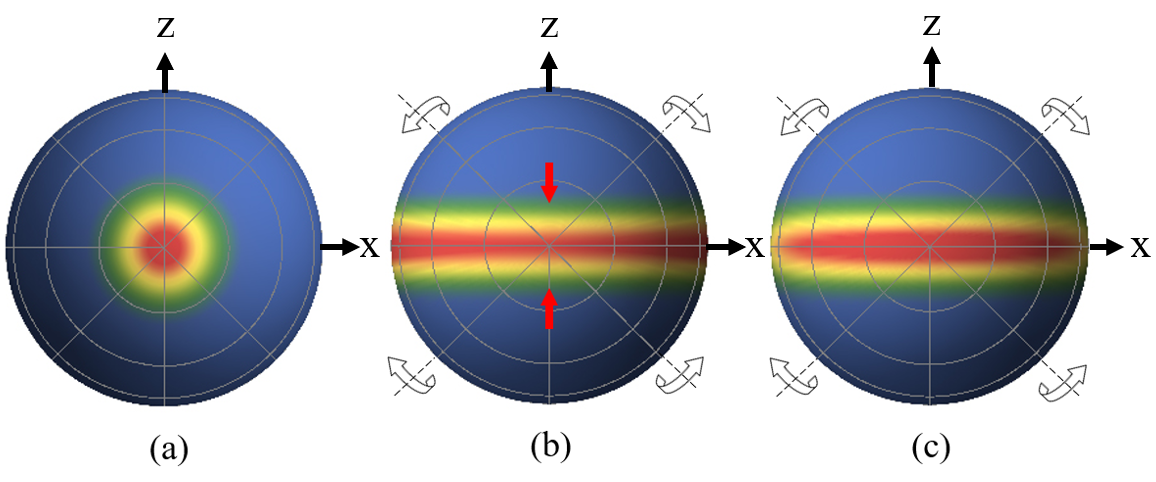
\includegraphics[scale=0.35]{Img/tat2.png}
	\bicaption{当S=20时,准概率分布(quasi-probability distribution, QPD)表示出的双轴反扭曲模型所引起的态演化。图中的密度通过$Q(\theta,\phi)$最大值$Q_{max}$进行了归一化。(a)显示初始相干自旋态$\ket{\theta=\pi/2,\phi=0}(Q_{max}=1)$。(b)和(c)显示由$U=exp[-i\mu(S_{\pi/2,\pi/4}^2-S_{\pi/2,-\pi/4}^2)/4]$产生的双轴反扭曲模型的态; (b)最优压缩出现在$\mu=0.203(Q_{max}=0.252)$; (c)显示在$\mu=0.248(Q_{max}=0.187)$的过度扭曲,QPD分裂为两部分。}
	{State evolutions by two-axis countertwisting in terms of the quasiprobability distribution (QPD) on the sphere for S=20. 
		The densities of the figures are normalized by the maximum value $Q(\theta,\phi)$ of $Q(\theta,\phi)$. 
		(a) shows the initial coherent spin state $\ket{\theta=\pi/2,\phi=0}(Q_{max}=1)$. 
		(b) and (c) are two-axis countertwisted states generated by the unitary transformation $U=exp[-i\mu(S_{\pi/2,\pi/4}^2-S_{\pi/2,-\pi/4}^2)/4]$; 
		(b) optimally squeezed at $\mu=0.203(Q_{max}=0.252)$ and (c) excessively twisted at $\mu=0.248(Q_{max}=0.187)$, where the QPD splits into two parts.}
	\label{figure6}
\end{figure}

双轴扭曲与单轴扭曲相比有以下的优点:在整个演化过程中,最佳压缩角度始终不变;压缩度比单轴扭曲模型高。单轴扭曲模型的压缩参数的最小值为$\xi_R^2\propto1/N^{2/3}$,而双轴扭曲可以达到海森堡极限$1/N$。


\vbox{}
\section{量子纠缠态}
\vbox{}
量子纠缠是一种量子力学现象,其中两个或更多粒子的量子态必须相互参照描述,即使各个物体可以在空间上分开。
它是量子信息中一个基本概念,也是几乎所有量子信息处理中不可缺少的理论支撑,其在不同学科之间起到了一个桥梁的作用,利用它我们可以很好的研究一些由大量粒子组成的系统的的统计性质。在这一节中,我们主要介绍了量子纠缠的基本概念、度量方式、应用、以及常见的两粒子系统之间的量子纠缠态。

\subsection{量子纠缠的概念}
纠缠态的概念首先是由薛定谔于1935年发表的薛定谔的猫态一文\cite{article1935}中提出的。这篇文章里讲述了一个假想实验,在一个密封的箱子里有一只猫,箱子里有一个装满毒气的瓶子,而装毒气的瓶子是否破碎完全由一个放射装置控制。假设这个放射装置里的放射元素发生衰变的概率是50$\%$,也就是说如果里面的放射性元素发生衰变的话就会触动机关,毒药瓶就会破碎放出毒气,则猫被毒死。否则,则猫是活着的。薛定谔用如下的表达式来描述这个活猫和死猫的复合系统:
\begin{align}
\ket{\Psi}=\alpha\ket{live\  cat}\ket{\uparrow}+\beta\ket{dead\  cat}\ket{\downarrow},|\alpha|^2+|\beta|^2=1,
\end{align}
其中$|\alpha|^2$表示猫活着的概率,$|\beta|^2$表示猫死了的概率。从上面的表达式我们可以看出来,猫以不同的概率同时处于这两种状态,即猫同时处于活着和死了的叠加态。而只有我们打开这个箱子去观测它我们才能知道猫到底是死了还是活着。这么一来,猫的生死就无法依赖于观测之前的“客观事实”,而是依赖于我们的观测,这是哥本哈根学派给出的解释。由于量子世界与我们所生活的宏观世界的生活经验差异之大,所以一时间人们很难接受。而人们对于这种量子描述的质疑主要来自于量子纠缠表现出来的非局域性,于是在这种质疑下人们提出了量子纠缠的概念。
\subsection{几种常见纠缠态}
由于不同数目的粒子都有可能纠缠在一起,所以按照纠缠粒子数的多少可以将纠缠态分为以下几类:在两粒子纠缠的系统中,我们将这种纠缠态称之为Bell态\cite{bell1964einstein}(由于Bell等人提出了著名的Bell不等式的缘故)。在三粒子系统中则有两种纠缠模型,分别称之为GHZ态\cite{greenberger2000similarities}和W态\cite{dur2000three}。而对于多粒子的系统,则分别有对应的多粒子GHZ态,多粒子W态,Cluster态,Dicke态等其他的一些纠缠态。下面简单介绍一下。
\subsubsection{Bell态}
Bell态是爱尔兰的物理学Bell提出来用于描述两个qubit系统的最大纠缠态,其具体的表达式为
\begin{align}\label{eq2241}
\begin{split}
\ket{\psi^{\pm}}&=\frac{1}{\sqrt{2}}(\ket{0}_A\ket{1}_B\pm\ket{1}_A\ket{0}_B)\\
\ket{\phi^{\pm}}&=\frac{1}{\sqrt{2}}(\ket{0}_A\ket{0}_B\pm\ket{1}_A\ket{1}_B)
\end{split}
\end{align}
上面的这四个态统称为一组Bell基,它是四维Hilbert空间的正交归一完备的基矢。如果用这组Bell作为测量基矢对系统进行测量操作,这个过程叫做Bell基测量。我们接下来证明一下Bell态具有非定域关联性,先假设A和B构成了一个处于Bell态$\ket{\psi^\pm}$的系统,我们先对A进行量子测量,于是我们可能得到两种不同的测量结果:粒子A处于1态或0态,如果是A则B必定是0,反之B为1。也就是说这两个粒子之间有某种关联,即当我们对一个粒子进行测量的时候,另外一个粒子的测量结果我们也会得到。
\subsubsection{GHZ纠缠态}
GHZ态是一种三粒子纠缠系统,由三名科学家一起提出来的\cite{greenberger2000similarities},它的表达式为
\begin{align}\label{eq2242}
\ket{GHZ}=\frac{1}{\sqrt{2}}(\ket{0}_A\ket{0}_B\ket{0}_C\pm\ket{1}_A\ket{1}_B\ket{1}_C),
\end{align}
从公式(\ref{eq2242})我们可以看出来GHZ态也具有非局域关联性,即当测量其中一个粒子处于$\ket{1}$($\ket{0}$)态时,其它的两个也注定处于$\ket{1}$($\ket{0}$)态。
\subsubsection{W纠缠态}
W纠缠态是另外一种三粒子纠缠态,它的表达式为
\begin{align}\label{eq2243}
\ket{W}=\frac{1}{\sqrt{3}}(\ket{0}_A\ket{1}_B\ket{1}_C+\ket{1}_A\ket{0}_B\ket{1}_C+\ket{1}_A\ket{1}_B\ket{1}_C),
\end{align}
从上式我们可以看出,不同于GHZ态,当其中一个粒子处于$\ket{1}$态时,另外两个粒子将塌缩到两粒子纠缠态$\ket{1}\ket{0}+\ket{0}\ket{1}$。由于此性质,因此W态已经被广泛的运用到量子信息处理方案中\cite{lee2006quantum,xi2007controlled,hao2009scheme}。

\subsection{量子纠缠的度量}
类似于压缩态用压缩度来度量其压缩程度一样,我们也用纠缠度来度量量子纠缠的程度。纠缠度量描述的方法也各不一样,这里介绍几种比较常见的度量方法。
\subsubsection{约化熵纠缠}
假如系统是两体纯态,那么约化熵纠缠的定义\cite{phoenix1990periodicity,phoenix1991establishment}为
\begin{align}\label{eq2244}
E=S_N(\rho_A)=S_N(\rho_B),
\end{align}
其中$S(\rho_A)=-Tr(\rho_A\log\rho_A)$和$S(\rho_B)=-Tr(\rho_B\log\rho_B)$分别表示系统A,B的约化密度矩阵的化密度矩阵的冯·诺依曼嫡,其中对数函数的底2,$\rho_A=Tr_B(\ket{\Psi}_{AB}\bra{\Psi})$,$\rho_B=Tr_A(\ket{\Psi}_{AB}\bra{\Psi})$。如果我们已经知道系统A得约化密度矩阵$\rho_A$的本征值$\lambda_i$,则$S_N(\rho_A)$就要写为如下的形式:
\begin{align}\label{eq2245}
S_N(\rho_A)=-\sum_i\lambda_i\log\lambda_i,
\end{align}

如果在两体纯态基础上,考虑两体混合态的约化嫡,则有如下定义:
\begin{align}\label{eq2246}
E_I=S(\rho_A)+S(\rho_B)-S(\rho_{AB}),
\end{align}
把$E_I$定义为相对信息嫡。
\subsubsection{形成纠缠}
在一个两体系统中,如果体系量子态可以用$\rho_{AB}=\sum_i p_i\ket{\Psi_i}_{AB}\bra{\Psi_i}$表示,那么纠缠的定义可以写为\cite{zhang2007thermal}:
\begin{align}\label{eq2247}
E_F(\rho_{AB})=\mathop {\min }\limits_{{{\left\{ {{p_i},{{\left| {{\Psi _i}} \right\rangle }_{AB}}} \right\}}_i}} \sum\limits_i {{p_i}{E_p}({{\left| {{\Psi _i}} \right\rangle }_{AB}})} ,
\end{align}
其中min的下标表示所有$\rho_{AB}$的集合。$E_p(\ket{\Psi_i}_{AB})$表示$\ket{\Psi_i}_{AB}$
的约化熵纠缠。

Wootters等人后面又提出了进一步反映量子态纠缠度的概念-并发度。如果一个两体系统的密度矩阵为$\rho_{AB}$,那么它们之间的纠缠可以表示成如下的形式:
\begin{align}\label{eq2248}
E_F(\rho_{AB})=H(\frac{1+\sqrt{1-C^2(\rho_{AB})}}2),
\end{align}
在上式中$H(p)=-p\log_2p-(1-p)\log_2(1-p)$,$C(\rho_{AB})$就是并发度,具体的表达式为$C(\rho_{AB})=max{0,\lambda_1-\lambda_2-\lambda_3-\lambda_4}$,其中$\lambda_i$(i=1,2,3,4,且有$\lambda_1\ge\lambda_2\ge\lambda_3\ge\lambda_4$)
表示$R=\rho_{AB}(\sigma_y^A\otimes\sigma_y^B)\rho_{AB}^*(\sigma_y^A\otimes\sigma_y^B)$的本征值平方根。

如果系统的密度矩阵表示为
\begin{equation}\label{eq2249}
\rho_{A B}=\left( \begin{array}{cccc}{\rho_{11}} & {0} & {0} & {\rho_{14}} \\ {0} & {\rho_{22}} & {\rho_{23}} & {0} \\ {0} & {\rho_{32}} & {\rho_{33}} & {0} \\ {\rho_{41}} & {0} & {0} & {\rho_{44}}\end{array}\right)
\end{equation}

那么体系的并发度就可以具体表示为
\begin{equation}\label{eq2250}
C\left(\rho_{A B}\right)=2 \max \left\{0,\left|\rho_{23}-\sqrt{\rho_{11} \rho_{44}}\right|,\left|\rho_{14}-\sqrt{\rho_{22} \rho_{33}}\right|\right\}
\end{equation}

\subsection{量子纠缠的应用}
量子纠缠是一种很重要的资源,其在量子隐形传态,量子秘钥分发等方面有着很重要的应用。

\subsubsection{量子隐形传态}
在1993年Bennett等人\cite{bennett1993teleporting}提出了量子隐形传态的协议,其对于任意未知量子态之间的传输是通过利用EPR纠缠的方法来实现的。该协议的主要思想是空间上相隔很远的两个通讯者之间分享一个纠缠态,通过利用这个纠缠态并借助经典通信渠道,便可以全部的分享一个量子态。

下面我们具体的介绍一下这个协议的工作原理:

假设通讯的双方为Alice和Bob,现在Alice想把1粒子的信息发送给Bob,未知的量子态表示为:
\begin{align}\label{eq2251}
\ket{\Psi}_1=\alpha\ket{0}_1+\beta\ket{1}_1,
\end{align}
其中$\alpha,\beta$为概率幅,满足归一化条件:$\alpha^2+\beta^2=1$。由于Alice和Bob之间共享一对EPR纠缠态,这对纠缠态的表示为
\begin{align}\label{eq2252}
\ket{\Psi}_{23}=\frac{1}{\sqrt{2}}(\ket{0}_2\ket{0}_3+\ket{1}_2\ket{1}_3),
\end{align}
则Alice和Bob所有粒子构成系统的总的状态可以表示为:
\begin{equation}
\begin{aligned} | \Psi \rangle_{123} &=| \Psi \rangle_{1} \otimes | \Psi \rangle_{23} \\ 
&=\frac{1}{\sqrt{2}}(\alpha\ket{0}_1+\beta \ket{1}_1 ) \otimes( \ket{0}_2\ket{0}_3+\ket{1}_2\ket{1}_3 ) \\
 &=\frac{\alpha}{\sqrt{2}}( \ket{0}_1\ket{0}_2\ket{0}_3+\ket{0}_1\ket{1}_2\ket{1}_3)+\frac{\beta}{\sqrt{2}}( \ket{1}_1\ket{0}_2\ket{0}_3+\ket{1}_1\ket{1}_2\ket{1}_3 ) \end{aligned}
\end{equation}

接下来我们将粒子1和2分解到4个Bell基上:
\begin{equation}
\begin{aligned} 
\ket{\Phi^{\pm}}_{12}&=\frac12(\ket{0}_1\ket{0}_2\pm\ket{1}_1\ket{1}_2)\\
\ket{\Phi^{\pm}}_{12}&=\frac12(\ket{0}_1\ket{1}_2\pm\ket{1}_1\ket{0}_2),
\end{aligned}
\end{equation}
则这个系统可以重新表示为
\begin{equation}
\begin{aligned} 
\ket{\Psi}_{123}=&[\ket{\Phi^{+}}_{12}(\alpha\ket{0}_3+\beta\ket{1}_3)+\ket{\Phi^{-}}_{12}(\alpha\ket{0}_3-\beta\ket{1}_3)\\
                     +&  \ket{\Psi^{+}}_{12}(\alpha\ket{1}_3+\beta\ket{0}_3)+\ket{\Psi^{-}}_{12}(\alpha\ket{1}_3-\beta\ket{0}_3)]/2,
\end{aligned}
\end{equation}
Alice对粒子1和2进行Bell态测量,然后把测量结果反馈给Bob,  Bob根据Alice反馈的结果,对所拥有的3号粒子进行幺正操作,便可以得到未知态$\ket{\Psi}_3$。

量子隐形传态有以下的几个特点:
(1)要完成量子隐形传态除了需要量子通道之外,还需要借助经典通道才能完成,因此,此过程不会超光速,也就不违背光速最大原理。
(2)在整个传态过程中,Alice需要对手中的粒子进行测量,测量以后这个粒子便不再处于原来的状态,因此整个过程也不违背量子不可克隆定理。
(3)由于量子纠缠态的非局域特性,整个过程不受空间的限制,所以通讯双方无需知道对方在哪里都可以进行。

总的来说,量子隐形传态传输的是量子信息,但其传输过程仍需要经典通道的协助,不过经典通道只是传达了测量结果。所以,未知量子态的传输并未加在任何的载体上,便可在一个地方突然消失,又在另一个地方突然出现。
\subsubsection{量子秘钥分发}
量子密钥分发(KQD)是一种安全的通信方法,它实现了基于量子力学成分的加密协议,它使通信双方产生只有他们自己知道共享随机秘钥,然后可以用于加密和解密消息。QKD的安全性依赖于自然的基本定律,这些定律不受增加计算能力,新攻击算法或量子计算机的影响,它可以抵御任意的强大窃听者。

1984年,Bennett和Brassard首次提出利用光子的偏振态来实现量子密钥分配的协议,又称为BB84协议\cite{bennett1984brassard}。在BB84协议中,首先选择有四个偏振方向的线性偏振单光子,四个偏振方向分别为水平方向、垂直方向45$^{\circ}$和135$^{\circ}$方向,这四个方向的光子态分别用$\ket{H}$、$\ket{V}$、$\ket{L}=1/\sqrt{2}(\ket{H}+\ket{V})$和$\ket{R}=1/\sqrt{2}(\ket{H}-\ket{V})$表示,这四个量子态之间都彼此正交,各自组成一对测量基,前两个态组成的基称为直测量基$\oplus$,后者称为斜测量基$\otimes$。

\begin{table}[htbp]
	\centering
		\bicaption{BB84协议中双方操作过程}{The operation process of both parties in the BB84 protocol}
	\begin{tabular}{|c|c|c|c|c|c|c|c|c|}
		\hline  % 在表格最上方绘制横线
		Alice's random bit              &0&1&1&0&1&0&0&1\\
		\hline  %在第一行和第二行之间绘制横线
		Alice's random sending basis    &$+$&$+$&$\times$&$+$&$\times$&$\times$&$\times$&$+$\\
		\hline  %在第一行和第二行之间绘制横线
		Photon polarization Alice sends &$\uparrow$&$\rightarrow$&$\searrow$&$\uparrow$&$\searrow$&$\nearrow$&$\nearrow$&$\rightarrow$\\
		\hline  %在第一行和第二行之间绘制横线
		Bob's random measuring basis    &$+$&$\times$&$\times$&$\times$&$+$&$\times$&$+$&$+$\\
		\hline  %在第一行和第二行之间绘制横线
		Photon polarization Bob measures&$\uparrow$&$\nearrow$&$\searrow$&$\nearrow$&$\rightarrow$&$\nearrow$&$\rightarrow$&$\rightarrow$\\
		\hline  %在第一行和第二行之间绘制横线
		PUBLIC DISCUSSION OF BASIS      &&&&&&&&\\
		\hline  %在第一行和第二行之间绘制横线
		Shared secret key               &0&&1&&&0&&1\\
		\hline  %在第一行和第二行之间绘制横线
	\end{tabular}
\end{table}
我们现在来看一下BB84协议的执行过程是怎么样的:首先Alice随机选择一种偏振光子用${\ket{H},\ket{V},\ket{L},\ket{R}}$,然后通过量子通道将其发送给Bobo。在发送之前,Alice和Bob约定好了给光子量子态$\ket{H}$、$\ket{R}$编码为0,光子量子态用$\ket{V}$、$\ket{L}$编码为1。随后Bob按照之前约定好的光量子态随机选择一种测量对自己接收到的量子态进行测量,并记录下测量结果。完了之后Bob通过公开信道将自己选择的测量基和测量结果告诉Alice。Alice通过将Bob的结果与自己的发送态和测量基进行比较,然后通过同样的通道告诉Bob哪些结果需要保留,哪些需要丢弃。

最后我们简单的分析一下量子密钥分发的安全性。假设在密钥传输的过程中存在着一个非法窃听者Eve,Eve首先通过技术手段窃取了Alice发送的量子态,然后随即选择了一组测量基对其进行测量。Eve有50\%的概率选对测量基和50\%的概率选错测量基。为了自己在窃取过程中不被发现,Eve冒充Alice将测量结果发送给Bob。结果,Bob最终将以正确率为$50\%\times 100\%+50\%\times 50\%=75\%$的概率保留正确的结果,即窃听者Eve引起的误码率为25\%。如果Alice向Bob发送N个量子态,那么误码率为0.25$^N$,当N很大时,误码率接近于0,因此,我们可以下结论:量子密钥分配具有很高的安全性。

%\subsection{量子纠缠的产生}
\vbox{}
\section{海森堡-朗之万理论}\label{section23}
\vbox{}
利用我们前面第\ref{paf}小节得到的哈密顿量,我们可以很容易的写出海森堡-朗之万方程\cite{scully1998quantum}。对于一个跃迁频率为$\omega$的原子系综和腔场耦合的系统,其总的哈密顿量可以表示为如下的形式
\begin{align}
H = \frac{1}{2}\hbar {\omega _0}\sum\nolimits_j {\sigma _j^z}  + \hbar {\omega _0}{a^\dag }a + \hbar \lambda \sum\nolimits_j {\Theta \left( {t - {t_j}} \right)} \left( {\sigma _j^ + a + \sigma _j^ - {a^\dag }} \right),\label{eq58}
\end{align}
其中$\Theta \left( {t - {t_j}} \right)$一般称做阶跃函数。

在上面的哈密顿量中,$\sigma_j^+$和$\sigma_j^-$分别表示产生算符和湮灭算符。$\sigma_j^-$是第$j$个原子的布居差。根据海森堡方程我们可以计算得出如下的原子与场的演化方程
\begin{align}\label{eq59}
\begin{split}
\dot a &=  - \frac{\gamma }{2}a - i\lambda \sum\nolimits_j {\Theta \left( {t - {t_j}} \right)} \sigma _j^ +  + {F_a}\left( t \right),\\
\dot \sigma _j^ + & =  - \frac{\gamma }{2}\sigma _j^ +  + i\lambda \Theta \left( {t - {t_j}} \right)\left[ {\sigma _j^a - \sigma _j^b} \right]a + {F_{\sigma _j^ + }}\left( t \right),\\
\dot \sigma _j^a &=  - \gamma \sigma _j^a + i\lambda \Theta \left( {t - {t_j}} \right)\left[ {{a^\dag }\sigma _j^ +  - a\sigma _j^ - } \right] + {F_{\sigma _j^a}}\left( t \right),\\
\dot \sigma _j^b &=  - \gamma \sigma _j^b + i\lambda \Theta \left( {t - {t_j}} \right)\left[ {{a^\dag }\sigma _j^ +  - a\sigma _j^ - } \right] + {F_{\sigma _j^b}}\left( t \right),
\end{split}
\end{align}
其中$\gamma$是原子自发辐射的衰减率,我们假设激发态衰变的两个基态的衰减率一样。$\sigma _j^a$和$\sigma _j^b$是$a$态和$b$态的原子布居算符,$F$是对应的噪声算符。接下来,规定算符的序,然后给出对应的$c$数,$a \to \alpha $,$\sigma _j^ +  \to v$,$\sigma _j^a \to {z_a}$,$\sigma _j^b \to {z_b}$ ,最后将公式(\ref{eq59})可以变为$c$数的朗之万方程
\begin{align}\label{eq60}
\begin{split}
\dot \alpha  &=  - \frac{\gamma }{2}a - i\lambda \sum\nolimits_j {\Theta \left( {t - {t_j}} \right)} \sigma _j^ +  + {F_\alpha }\left( t \right),\\
\dot v &=  - \frac{\gamma }{2}v + i\lambda \Theta \left( {t - {t_j}} \right)\left[ {{z_a} - {z_b}} \right]\alpha  + {F_v}\left( t \right),\\
{{\dot z}_a} &=  - \gamma {z_a} + i\lambda \Theta \left( {t - {t_j}} \right)\left[ {{\alpha ^\dag }v - \alpha {v^\dag }} \right] + {F_{{z_a}}}\left( t \right),\\
{{\dot z}_b} &=  - \gamma {z_b} + i\lambda \Theta \left( {t - {t_j}} \right)\left[ {{\alpha ^\dag }v - \alpha {v^\dag }} \right] + {F_{{z_b}}}\left( t \right),
\end{split}
\end{align}
上面的噪声项满足如下的式子
\begin{align}\label{eq61}
\begin{split}
\left\langle {{F_z}\left( t \right)} \right\rangle  &= 0,\\
\left\langle {{F_z}\left( t \right){F_y}\left( {t'} \right)} \right\rangle  &= 2{D_{xy}}\delta \left( {t - t'} \right),
\end{split}
\end{align}
其中$D_{xy}$是扩散系数,可以利用广义爱因斯坦关系\cite{PhysRevA.76.033804,JOB}来计算。

我们首先将上述的朗之万方程写成如下的一般形式
\begin{align}
{\dot A_\mu } = {D_\mu }(t) + {F_\mu }(t),\label{eq62}
\end{align}
其中$D_\mu(t)$是$A_\mu(t)$的漂移算符,$F_\mu(t)$是相应的噪声项,其库平均为零,即$\braket{F_u(t)}=0$ 。

同样我们也可以写出噪声算符的时间平均值
\begin{align}
\left\langle {{F_\mu }\left( t \right){F_\nu }\left( {t'} \right)} \right\rangle  = 2{D_{\mu \nu }}\delta \left( {t - t'} \right),\label{eq63}
\end{align}
为了得到系数$2D_{\mu\nu}$,我们需要引入恒等式
\begin{align}
{A_\mu }\left( t \right) = {A_\mu }\left( {t - \Delta t} \right) + \int_{t + \Delta t}^t {dt'} {\dot A_\mu }\left( t \right),\label{eq64}
\end{align}
于是我们得到了系统的噪声关联函数
\begin{align}
\left\langle {{A_\mu }\left( t \right){F_\nu }\left( t \right)} \right\rangle  = \left\langle {{A_\mu }\left( {t - \Delta t} \right){F_\nu }\left( t \right)} \right\rangle  + \int_{t - \Delta t}^t {dt'} \left\langle {{D_\mu }\left( {t'} \right) + {F_\mu }\left( t \right)} \right\rangle {F_\nu }\left( t \right),\label{eq65}
\end{align}
然后我们将方程(\ref{eq56})代入式(\ref{eq65}),我们可以得到
\begin{align}
\left\langle {{A_\mu }\left( t \right){F_\nu }(t)} \right\rangle  = \left\langle {{D_{\mu \nu }}} \right\rangle ,\label{eq66}
\end{align}
通过同样的方法,也有
\begin{align}
\left\langle {{F_\nu }(t){A_\mu }\left( t \right)} \right\rangle  = \left\langle {{D_{\mu \nu }}} \right\rangle ,\label{eq67}
\end{align}
最后整理到一起
\begin{align}\label{eq68}
\begin{split}
\frac{d}{{dt}}\left\langle {{A_\mu }\left( t \right){A_\nu }\left( t \right)} \right\rangle  
&= \left\langle {{{\dot A}_\mu }\left( t \right){A_\nu }\left( t \right)} \right\rangle  + \left\langle {{A_\mu }\left( t \right){{\dot A}_\nu }\left( t \right)} \right\rangle \\
& = \left\langle {{D_\mu }\left( t \right){A_\nu }\left( t \right)} \right\rangle  + \left\langle {{F_\mu }\left( t \right){A_\nu }\left( t \right)} \right\rangle {\rm{ + }}\\
&\quad\left\langle {{A_\mu }\left( t \right){D_\nu }\left( t \right)} \right\rangle  + \left\langle {{A_\mu }\left( t \right){F_\nu }\left( t \right)} \right\rangle ,
\end{split}
\end{align}
最后我们便可以得到一般情况下的爱因斯坦关系
\begin{align}
2\left\langle {{D_{\mu \nu }}} \right\rangle  =  - \left\langle {{A_\mu }\left( t \right){D_\nu }\left( t \right)} \right\rangle  - \left\langle {{D_\mu }\left( t \right){A_\nu }\left( t \right)} \right\rangle  + \frac{d}{{dt}}\left\langle {{A_\mu }\left( t \right){A_\nu }\left( t \right)} \right\rangle ,\label{eq69}
\end{align}



\chapter{在光学腔中通过非共振受激拉曼制备自旋压缩态}\label{chapter3}
\vbox{}\vbox{}
\section{引言}
\vbox{}
%量子光学是研究光场的量子统计信息、量子相干性质,以及光与物质(原子,离子等)相互作用中的量子效应的一门学科。目前研究很热门的一个课题就是研究光场与原子系综发生相互作用时引发的量子特性的变化,尤其是原子系综的压缩效应,研究原子系综压缩效应不仅能反映与光场相互作用的量子效应,而且在精密测量、引力波探测、原子钟和量子通信等方面都有着很广泛的应用,因此原子压缩态的研究备受人们的青睐。本章主要研究了在$\Lambda$型三能级原子与单模光场相互作用的系统中的压缩特性,并且讨论了拉比频率等参数对其压缩特性的影响。



自旋压缩态\cite{PRA1993Kitagawa}在量子信息处理\cite{JPB2008qf,JPA2014qf,Teles2015}和精密测量\cite{PRA2007pm,PRL2011pm,PRL2016pm}中发挥着很重要的作用。最近,已经提出了各种方法\cite{PRA2002SS,PRA2012LI,PRL2013DT,NJP2017J-Borregaard,PRA2017Wang,NJP2010ex,PRL2010ex} 来制备这样的态,包括集体自旋的量子非破坏性测量\cite{NJP1998qnd,PRA1999qnd,PRL2000qnd,PRL2000Duan,PRL2016qnd},基于单轴扭曲\cite{PRA1993Kitagawa,PRA2002SS}或双轴扭曲\cite{PRA2017Wang,NJP2017J-Borregaard}的自旋之间的非线性相互作用等。基于QND的方法具有实现简单的优点,而另一方面,它还具有难以产生高度自旋压缩态的缺点,因为其具有$N$个原子总数的低效降噪缩放比例$\propto N^{-1/2}$。相反,基于非线性相互作用的方法已被证明比QND方案更有效 \cite{PRA1993Kitagawa},因为OAT的自旋压缩的理论极限为$\propto N^{-2/3}$,并且TAT的降噪甚至可以达到海森堡$\propto N^{-1}$。

迄今为止,人们已经注意到在原子系统中实现OAT和TAT演化。在用于实现各个自旋之间的非线性相互作用的研究最多的系统是空腔中的原子系统\cite{PRA2002SS,NJP2017J-Borregaard,PhysRevA.89.023838,PhysRevLett.110.120402,PhysRevA.86.013828,PhysRevA.77.063811,PhysRevA.75.013804,PhysRevLett.88.243602}。其中,S\o{}ndberg 和 M\o{}lmer的一项令人印象深刻的工作提出通过双受激拉曼散射实现OAT演化\cite{PRA2002SS}。他们表明,两个经典的驱动场和一个真空腔模式可以同时以一种类似于光学参量放大中相关光子对发射的方式发出一对原子,从而产生单个自旋之间的纠缠这也是OAT自旋压缩的本质。这种方法的优点是它可以产生单一的OAT自旋压缩,如\cite{Braverman_2018}所示,它可以产生比非单一压缩更好的时钟稳定性。另一个优点是,由于原子-光耦合\cite{PhysRevLett.84.4232,PhysRevLett.86.783}的集体增强效应,该方法原则上可以在任何光学腔中工作,例如坏腔。最近,该方案也被Borregaard等人\cite{NJP2017J-Borregaard}通过增加两个额外的经典驱动场扩展到TAT自旋压缩的情况。

我们通过适当改变初始输入原子态,可以通过使用原子和光之间的单个SRS相互作用来实现OAT自旋压缩。我们的方案与\cite{PRA2002SS}中的机制相反,由于所提出的方法仅需要单个经典驱动场,因此可以显着简化可能的实验实现。通过在OAT自旋压缩期间向自旋极化方向添加旋转来适当地相干控制集体自旋,表明OAT演化可以转换为TAT,从而导致更快更强的压缩。与使用四个激光场将原子系统驱动到TAT压缩自旋状态的方法\cite{NJP2017J-Borregaard}相比,我们的TAT协议具有实验资源成本更低和实现更简单的优点。进一步的研究表明,对于诸如原子衰变的现实缺陷,本方案可以变得稳健。与伪角动量算子连接原子的基态和激发态的工作相比,我们连接两个基态平面,因此具有长相干时间的优点。

本章其余部分的结构如下。在第二节中,我们介绍了自旋压缩态产生的理想模型,第三节我们分析噪声对方案的影响和实验的可行性。第四节包含简短的结论。



\vbox{}
\section{压缩态的产生}
\vbox{}

我们考虑在单模光学腔中有一个三能级的原子系综与之相互作用,其原子数为N,能级结构如图\ref{figure7}所示,$\ket{1}$和$\ket{2}$分别表示原子的两个基态,$\ket{3}$为原子的激发态。
\begin{figure}[htbp]
	\centering
	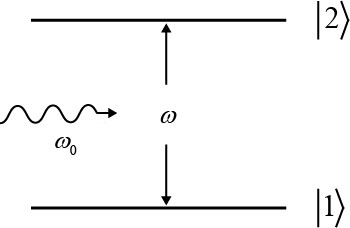
\includegraphics[scale=0.5]{Img/Fig_1.pdf}
	\bicaption{自旋压缩的方案示意图。 激光束进入光学腔并与$x$偏振的集体自旋相互作用以实现基态$\ket{1}$和激发态$\ket{3}$之间的非共振耦合。基态$\ket{2}$通过最初处于真空态的腔模式耦合到激发态$\ket{3}$。绝热消除激发态导致集体自旋的非线性OAT演化。沿着$x$方向向集体旋转并添加均匀磁场B使得能够将OAT转换为TAT自旋压缩。}	
	{Schematic setup for spin squeezing. A laser beam enters the optical cavity and interacts with an $x$-polarized collective spin to realize the off-resonance coupling between the ground state $|1\rangle$ and the exited state $|3\rangle$. The ground state $|2\rangle$ is coupled to the excited state $|3\rangle$ by a cavity mode which is initially in a vacuum state. Adiabatic elimination of the exited state leads to a nonlinear OAT evolution for the collective spin. Adding a homogeneous magnetic field $B$ to the collective spin along the $x$ direction enables the conversion of OAT into TAT spin squeezing.}
	\label{figure7}
\end{figure}
原子被一个频率为$\omega$,拉比频率为$\Omega$的强经典场驱动,驱动场作用在$\ket{1}$和$\ket{3}$的原子跃迁上(其能级差对应的频率为$\omega_{13}$)。腔中的量子场$c$作用在$\ket{2}$和$\ket{3}$的原子跃迁上(其能级差对应的频率为$\omega_{23}$),量子场的频率为$\omega_0$。腔模最初处于真空态,原子最初是处在它们基态的叠加态上,形成自旋相干态(coherent spin state, CSS)$\ket{CSS}=2^{N/2}(\ket{1}+\ket 2)^{\otimes N}$,算符$\hat{S}_x$的本征态的本征值为N/2。经典场从$\ket 1\to\ket 3$谐振的失谐量是$\Delta$[其能极差为$\omega_{13}$(下文中我们取$\hbar=1$)],而量子场与非共振原子跃迁$\ket 1\to\ket 3$(其能极差为 ${\omega _{23}} \equiv {\omega _{13}}$)的失谐量是$\Delta+\delta$,其中$\delta=\omega-\omega_0$是双光子失谐[见图\ref{figure7}]。取基态$\ket{1}$为零势能点,则描述系统的哈密顿量可以写为
\begin{align}
\hat H = {\omega _0}{\hat c^\dag }c + {\sum _k}{\omega _{13}}\ket{3}_k\bra{3}+ {\sum _k}\left( {\frac{\Omega }{2}{e^{ - i\omega t}}\ket{3}_k\bra{1} + g\hat c\ket{3}_k\bra{2} + h.c.} \right),\label{eq441}
\end{align}
其中前两项分别描述腔场和原子的能量,最后一项描述光与原子之间的相互作用,其耦合强度$g=d\sqrt{\omega_0/2\pi\epsilon_0V_0}$,其中$d$是$\ket 2\to\ket 3$的偶极矩,$\epsilon_0$是真空介电常数,$V_0$是模的体积。定义$\hat{\sigma}_{\mu\nu}=\sum_k\ket{\mu}_k\bra{\nu}(\mu,\nu\in{1,2,3})$ ,则体系的哈密顿量可简化为
\begin{align}
\hat H = {\omega _0}{\hat c^\dag }c + {\omega _{13}}{\hat \sigma _{33}} + \frac{\Omega }{2}{e^{ - i\omega t}}{\hat \sigma _{31}} + g\hat c{\hat \sigma _{32}} + \frac{{{\Omega ^*}}}{2}{e^{i\omega t}}{\hat \sigma _{13}} + {g^*}{\hat \sigma _{23}}{\hat c^\dag },\label{eq442}
\end{align}
在$\hat H_0= \omega_0\hat c^\dag \hat c + \omega_{ae}\sigma_{ee}+ \omega_{ab}\sigma_{bb}$的旋转框架下,对公式(\ref{eq442})的哈密顿量进行旋转,得到
\begin{align}\label{eq443}
\begin{split}
\tilde{ \hat{ H}} &= {e^{i{{\hat H}_0}t/\hbar }}\hat H{e^{ - i{{\hat H}_0}t/\hbar }} - {{\hat H}_0}\\
&= \Delta {{\hat \sigma }_{33}} + \frac{\Omega }{2}{{\hat \sigma }_{31}} + g\hat \varepsilon {{\hat \sigma }_{32}} + \frac{{{\Omega ^*}}}{2}{{\hat \sigma }_{13}} + g{{\hat \sigma }_{23}}{{\hat \varepsilon }^\dag },
\end{split}
\end{align}
式中我们定义了一个新算符$\hat \varepsilon  = \hat c{e^{i\delta t}}$。根据哈密顿量,我们可以计算出光和原子的海森堡方程,得到如下的Maxwell-Bloch方程
\begin{align}
{\dot {\hat {\sigma}} _{11}}& = i\frac{\Omega }{2}{\hat \sigma _{31}} - i\frac{{{\Omega ^*}}}{2}{\hat \sigma _{13}},\label{eq444}\\
{\dot {\hat {\sigma}} _{22}} &= ig\hat \varepsilon {\hat \sigma _{32}} - i{g^*}{\hat \sigma _{23}}{\hat \varepsilon ^\dag },\label{eq445}\\
{\dot {\hat {\sigma}} _{12}}& = i\frac{\Omega }{2}{\hat \sigma _{32}} - i{g^*}{\hat \sigma _{13}}{\hat \varepsilon ^\dag },\label{eq446}\\
{\dot {\hat {\sigma}} _{13}} &=  - i\Delta {\hat \sigma _{13}} - i\frac{\Omega }{2}\left( {{{\hat \sigma }_{11}} - {{\hat \sigma }_{33}}} \right) - ig\hat \varepsilon {\hat \sigma _{12}},\label{eq447}\\
{\dot {\hat {\sigma}} _{23}}& =  - i\Delta {\hat \sigma _{23}} - i\frac{\Omega }{2}{\hat \sigma _{21}} - ig\hat \varepsilon \left( {{{\hat \sigma }_{22}} - {{\hat \sigma }_{33}}} \right),\label{eq448}\\
{\dot {\hat {\sigma}} _{33}} &= i\frac{{{\Omega ^{\rm{*}}}}}{2}{\hat \sigma _{13}} - i\frac{\Omega }{2}{\hat \sigma _{31}} + i{g^{\rm{*}}}{\hat \sigma _{23}}{\hat \varepsilon ^ + } - ig\hat \varepsilon {\hat \sigma _{32}},\label{eq449}\\
\dot{ \hat{ \varepsilon}}  &=  - i{g^*}{\hat \sigma _{23}} + i\delta \hat \varepsilon ,\label{eq4410}
\end{align}
接下来,为了方便计算,我们做如下的假设:1.假设经典驱动场足够的弱。2.假设失谐量$\Delta\gg 1$。通过这样的假设,可以认为布居在激发态的原子数非常少,因此可以绝热消除掉激发态(${\hat{\sigma} _{33}} \simeq 0$)。大失谐还可以将$\hat{\sigma}_{13}$和$\hat{\sigma}_{23}$快速驱动到稳态,于是有${\hat \sigma _{13}} \simeq  - \left( {\Omega {{\hat \sigma }_{11}}/2 + g\hat \varepsilon {{\hat \sigma }_{12}}} \right)/\Delta $,${\hat \sigma _{23}} \simeq  - \left( {\Omega {{\hat \sigma }_{21}}/2 + g\hat \varepsilon {{\hat \sigma }_{22}}} \right)/\Delta $ 。我们进一步假设双光子失谐量足够大$\delta\gg 1$,使得在相互作用期间腔中没有产生显着的光子激发,这使得能够绝热地消除腔场,导致$\hat \varepsilon  =  - {g^*}\Omega {\hat \sigma _{21}}/2\Delta \delta $。基于这些假设,原子的基态方程可以写为
\begin{align}
{\dot{ \hat{ \sigma }}_{12}} =  - i{\kappa _0}{\hat S_z}{\hat \sigma _{12}} - i{\chi _0}{\hat \sigma _{12}},{\dot{ \hat{ \sigma }} _{11}} = {\dot{ \hat{ \sigma }} _{22}} = 0,\label{eq4411}
\end{align}
其中定义了 $\kappa_0=|\Omega|^2{|g|^2}/4{\delta\Delta^2}$ 和 $\chi_0 ={|\Omega|^2}/{4\Delta}$,以及角动量算符${\hat S_x} = (\hat{\sigma}_{12}+\hat{\sigma}_{21})/2$,${\hat S_y} = (\hat{\sigma}_{12}-\hat{\sigma}_{21})/2i$和${\hat S_z} = (\hat{\sigma}_{11}-\hat{\sigma}_{22})/2$。在伪角动量运算符的表述中,公式(\ref{eq4411})可以写为
\begin{align}
{{\dot {\hat S}}_x} &= {\kappa _0}\left( {{{\hat S}_y}{{\hat S}_z} + {{\hat S}_z}{{\hat S}_y}} +{{\hat S}_y}\right) + {\chi _0}{{\hat S}_y},\label{eq4412}\\
{{\dot {\hat S}}_y} &=  - {\kappa _0}\left( {{{\hat S}_x}{{\hat S}_z} + {{\hat S}_z}{{\hat S}_x}} +{{\hat S}_x}\right) - {\chi _0}{{\hat S}_x},\label{eq4413}\\
{{\dot {\hat S}}_z} &= 0,\label{eq4414}
\end{align}
从上面的这组方程,可以推断原子的动力学是由下式的有效哈密顿量产生的
\begin{align}
\hat H_{eff}=-\chi_0\hat S_z-\kappa_0(\hat S_z+\hat S_z^2),\label{eq4415}
\end{align}
从哈密顿量的形式我们知道这是一个OAT型的哈密顿量\cite{PRA1993Kitagawa}。(\ref{eq4415})式的第一项出现源于基态的AC-Stark平移,而其余项源于双光子非共振拉曼跃迁。通过考虑如图\ref{figure7}(b)所示的双拉曼过程,可以理解(\ref{eq4415})式中的非线性项的来源。假设所有原子在基态$\ket{1}$从经典驱动场吸收一个光子,并向腔场辐射一个光子,该光子被基态$\ket{2}$中的另一个原子吸收, 然后再次回到经典驱动场,这将导致从$\ket{12}\to\ket{21}$的有效转换。这双原子过程保持共振并导致自旋-自旋纠缠(以及自旋压缩)的产生。这种双原子翻转的动力学可以用有效的哈密顿量${\hat H_{eff}} = {\hat S_ - }{\hat S_ + } \propto \hat S_z^2$来描述。应该提到的是,原子发射的腔光子有可能被原子本身吸收,这抑制双原子过程。这就是为什么我们在这里采用相等的叠加自旋态作为输入态,因为在这种态下参与腔-光子反复吸收的原子数约为N/2,这可以极大地抑制自重吸收的影响,因此使双原子过程占主导地位。

我们可以很容易的求解方程(\ref{eq4412})得到
\begin{align}\label{eq4416}
\begin{split}
{{\hat S}_x}(t) =& {{\hat S}_ + }(0)\exp [i\mu ({{\hat S}_z} + 1/2 + \varphi /\mu )] \\
&+ \exp [ - i\mu ({{\hat S}_z} + 1/2 + \varphi /\mu )]{{\hat S}_ + }(0),
\end{split}
\end{align}
其中$\mu = -2\kappa_0 t$,$\varphi = -\varphi_0 t$和$\varphi_0=\chi_0+\kappa_0$。
将CSS在Dicke态的基上展开
\begin{align}
\ket{CSS} = \sum\nolimits_{m=-S}^S 2^{ - S}\sqrt {(2S)!/[(S + m)!(S - m)!]}\ket{m},\label{eq4417}
\end{align}
$S_x$的平均值通过计算可得
\begin{align}
\bra{CSS}\hat {S}_x\ket{CSS}=S \cos^{2S-1}{\frac {\mu}2} \cos{ \varphi },\label{eq4418}
\end{align}
对于$S\gg 1$和 $|\mu|,|\varphi|\ll1 $,有$\braket{S_x}\simeq S$。
这意味着在OAT相互作用之后,几乎所有原子仍然沿$x$方向极化。因此可以使用Holstein-Primakoff近似\cite{PhysRevA.58.1098}来定义新的原子量子变量$\hat {X}_a = {\hat S_y}/\sqrt {S_x} ,{\hat P_a} = {\hat S_z}/\sqrt {S_x} $,
满足$[\hat {X}_a,\hat {P}_a] = i$,对于CSS,有$\braket{\hat {X}_a}=\braket{\hat {P}_a}=0$
和归一化方差$(\Delta {\hat X}_a)^2 =(\Delta {\hat P}_a)^2= 1/2$。对于这种定义,方程(\ref{eq4413}-\ref{eq4414})可以表述为
\begin{align}
\hat X_a^{out} = \hat X_a^{in} + \alpha \hat P_a^{in} + \beta ,\hat P_a^{out} = \hat P_a^{in},\label{eq4419}
\end{align}
其中“in”和“out”是指相互作用之前和之后的原子,我们定义了耦合常数$\alpha=S\mu$和由于哈密顿量(\ref{eq4415})式中的线性项引起的位移参数$\beta=\sqrt{S}\phi$。显然,(\ref{eq4419})式中的自旋态是通过$\hat{P}_a^2$中哈密顿量的二次项来进行第一次压缩的自旋态,然后通过移位量$\beta$在相空间沿着$\hat{P}_a$方向来取代自旋压缩态而产生的。由于相空间中的位移运算(线性运算)不会减少由OAT演化\cite{RevModPhys.77.513}产生的原子-原子纠缠,因此当我们估计原子系统的压缩量时,可以忽略位移$\beta$。为了看看产生了多少压缩,我们通过幺正变换$\hat X_\theta^{out}=\exp(i\theta\hat H_{SR}) \hat X_a^{out}\exp(-i\theta\hat H_{SR})=\cos{\theta} \hat X_a^{in}+(\alpha\cos{\theta}+\sin{\theta})\hat P_a^{in}$绕$x$轴旋转自旋态,其中 $\hat H_{SR}=-2\hat S_x\simeq \hat X_a^2+\hat P_a^2$是自旋旋转哈密顿量\cite{PhysRevLett.91.060401}。关于$\theta$我们求方差$(\Delta\hat X_\theta^{out})^2$的最佳值,我们得到$\xi_{OAT}^2=2(\Delta\hat X_\theta^{out})^2=1+\alpha^2/2-(\alpha^4/4+\alpha^2)^{1/2}\Rightarrow \mathop{\lim}\limits_{\alpha\rightarrow \infty}1/\alpha^2$,其中$\theta=\arctan (2/\alpha)/2+\pi/2$。

如果可以将OAT转化为TAT,那么压缩量可以大大增加\cite{PhysRevLett.107.013601}。为此,我们在OAT相互作用过程中添加一个围绕$x$方向的旋转角频率$\Omega_0$ \cite{PhysRevA.92.063610,PhysRevA.87.051801,PhysRevA.91.053826}(可以通过沿$x$轴施加均匀磁场来实现,如图\ref{figure7}所示),于是将得到哈密顿量
\begin{align}\label{eq4420}
\begin{split}
\hat H_{TAT}&=\Omega_0\hat H_{SR}/2+\hat H_{eff}\\
            &=\Omega_0(\hat X_a^2+\hat P_a^2)/2-\kappa_0 S\hat P_a^2\\
            &=\kappa_0S(\hat X_a^2-\hat P_a^2)/2,
\end{split}
\end{align}
其中$\Omega_0=\kappa_0S$,这正是TAT型相互作用\cite{PRA1993Kitagawa},并以一个与耦合常数呈指数级缩放的速率压缩自旋涨落,即$\xi^2_{TAT}=\exp(-\alpha)$。与产生多项式压缩的OAT相比,TAT方法的指数缩放将极大地增强各个原子之间的纠缠,从而使我们能够对集体自旋进行很重要的控制。

\vbox{}
\section{噪声对方案的影响}
\vbox{}
到目前为止,我们忽略了噪声的影响。实际上,光子以一定的速率$\kappa$从空腔泄漏到环境中,激发态以辐射衰减率$\gamma_{13}=\gamma_{23}\equiv \gamma$衰减到基态。在存在衰变以及绕$x$方向旋转的情况下,原子算符的时间演变(更多详细推导参见附录\ref{appendix})可写为
\begin{eqnarray}
\frac{d}{{dt}}\left( {\begin{array}{*{20}{l}}
	{{{\hat X}_a}}\\
	{{{\hat P}_a}}
	\end{array}} \right) = \mathcal{G}\left( {\begin{array}{*{20}{l}}
	{{{\hat X}_a}}\\
	{{{\hat P}_a}}
	\end{array}} \right) - \sqrt S \left( {\begin{array}{*{20}{l}}
	{\varphi_0}\\
	\eta
	\end{array}} \right)
+ \sqrt {2\eta } \left( {\begin{array}{*{20}{l}}
	{{{\hat {\mathcal{F}}}_y}}\\
	{{{\hat {\mathcal{F}}}_z}}
	\end{array}} \right)\label{eq4421}
\end{eqnarray}
对于$r_0=\kappa/2\delta\ll 1$的情况
\begin{eqnarray}
\mathcal{G}={\Omega _0}\left( {\begin{array}{*{20}{c}}
	0&{ 1}\\
	-1&0
	\end{array}} \right) - 2S{\kappa _0}\left( {\begin{array}{*{20}{c}}
	0&1\\
	0&0
	\end{array}} \right) - \eta \left( {\begin{array}{*{20}{c}}
	1&0\\
	0&1
	\end{array}} \right),\label{eq4422}
\end{eqnarray}
在上式中$\eta=\chi_0\gamma/\Delta$表示原子的衰减参数,$\hat {\mathcal{F}}_y$和$\hat {\mathcal{F}}_z$是朗之万噪声算符,满足$\braket{\hat{\mathcal{F}}_y(t) \hat{\mathcal{F}}_z(t')}= i\delta(t-t')/2$和 $
\braket{\hat{\mathcal{F}}_y(t)\hat{\mathcal{F}}_y(t')}=\braket{\hat{\mathcal{F}}_z(t)\hat{\mathcal{F}}_z(t')}=\delta(t-t')/2$。$\mathcal{G}$的第一项表示原子由于$\Omega_0$绕$x$轴转动,$\mathcal{G}$中的第二项表示由光引起的相干OAT相互作用,而第三项表示由光泵浦引起的原子的横向衰变。注意,$\hat{P}_a$现在也以与$\eta$成比例的速率变化,这是由于强光场的作用导致基态布居数从$\ket{1}$转移到$\ket{2}$引起的。这个微分方程的解是
\begin{eqnarray}
\left( {\begin{array}{*{20}{l}}
	{\hat X_a^{out}}\\
	{\hat P_a^{out}}
	\end{array}} \right) &=& \mathcal{A}\left( t \right)\left( {\begin{array}{*{20}{l}}
	{\hat X_a^{in}}\\
	{\hat P_a^{in}}
	\end{array}} \right) - \mathcal{A}\left( t \right)\int_0^t {d\tau {\mathcal{A}^{ - 1}}\left( \tau  \right)} \nonumber\\
&&\times \left[ {\sqrt S \left( {\begin{array}{*{20}{l}}
		{{\varphi _0}}\\
		\eta
		\end{array}} \right) - \sqrt {2\eta } \left( {\begin{array}{*{20}{l}}
		{{{\hat {\mathcal{F}}}_y\left( \tau \right)}}\\
		{{{\hat {\mathcal{F}}}_z\left( \tau \right)}}
		\end{array}} \right)} \right],\label{eq4423}
\end{eqnarray}
其中齐次解为$\mathcal{A}\left( t \right)=\exp(\mathcal{G}t)$。对于OAT压缩的情况($\Omega_0=0$),我们有%$\mathcal{A}(t)={e^{ - \eta t}}\bigl(\begin{smallmatrix} 1 & \alpha \\\alpha & 0 \end{smallmatrix}\bigr)$
$$\mathcal{A}(t)={e^{ - \eta t}}\left(\begin{array}{cc}
1 & \alpha \\
\alpha & 0
\end{array}\right)$$
我们也可以直接从公式(\ref{eq4423})得到
\begin{eqnarray}
\hat X_a^{out} &=& \sqrt {1 - {\eta _0}} \left( {\hat X_a^{in} + \alpha \hat P_a^{in} + \beta' } \right) + \sqrt {{\eta _0}} {{\hat{\mathcal{F}}}_X},\label{eq4424}\\
\hat P_a^{out} &=& \sqrt {1 - {\eta _0}} \left( {\hat P_a^{in} + \beta ''} \right) + \sqrt {{\eta _0}} {{\hat{{\mathcal{F}}}}_P},\label{eq4425}
\end{eqnarray}
其中我们定义了参数$\eta_0=2\eta t, \beta'=\beta+\eta_0\alpha/4$和 $\beta''=\sqrt{S}\eta_0/2$,并使用了条件 $\eta_0\ll 1$。修改后的噪声算子的形式如下:$\hat{\mathcal{F}}_X=\frac{1}{\sqrt t}e^{-\eta t}\int_0^td\tau e^{\eta \tau}[\hat{\mathcal{F}}_y(\tau)-\alpha(\tau-t)/t\hat{\mathcal{F}}_z(\tau)],\hat{\mathcal{F}}_P=\frac{1}{\sqrt t}e^{-\eta t}\int_0^td\tau e^{\eta \tau}\hat{\mathcal{F}}_z(\tau)$, 我们也可以很容易的得到$\langle\hat{\mathcal{F}}_X\rangle=\langle \hat{\mathcal{F}}_P\rangle=0,\langle\hat{\mathcal{F}}_X \hat{\mathcal{F}}_P\rangle\simeq i(1-i\alpha/2)/2$,$\langle\hat{\mathcal{F}}_X^2\rangle\simeq (1+\alpha^2/3)/2$和 $\langle \hat{\mathcal{F}}_P^2\rangle\simeq 1/2$。借助于原子输入-输出关系(\ref{eq4424})和(\ref{eq4425}),我们可以计算方差$(\Delta\hat X_\theta^{out})^2$,从而得到方差的最优值
\begin{align}\label{eq4426}
\begin{split}
2(\Delta\hat X_\theta^{out})^2 =& 1 + \frac{{{\alpha ^2}}}{2}\left( {1 - \frac{2}{3}{\eta _0}} \right)\\
&- \sqrt {{{\left( {1 - \frac{2}{3}{\eta _0}} \right)}}^2\frac{{{\alpha ^4}}}{4} + {{\left( {1 - \frac{1}{2}{\eta _0}} \right)}}^2{\alpha ^2}}\\
&\Rightarrow \frac{1}{\alpha^2}+\frac{\eta_0}{3},\qquad\qquad\alpha \gg 1,
\end{split}
\end{align}
其中$\theta=\arctan [(2-\eta_0)/(\alpha-2\eta_0\alpha/3)]/2+\pi/2$。方程(\ref{eq4426})表明原子衰减设有一个极限,即$\eta_0/3$,达到了可以达到的最高压缩程度。对于位于腔体波腹上的原子,耦合常数$g$还可以方便地用激发态线宽$|g|^2=\gamma\kappa d_c/(4N)$表示\cite{phd11},腔体光学深度(optical depth, OD)为$d_c=\frac{2\mathcal {F}}{\pi}d_0=\frac{2\mathcal {F}}{\pi}\frac{N\sigma_0}{A_0}$,其中$\mathcal {F}$是腔体精细度,$d_0=N\sigma_0/A_0$是自由空间样品的OD值,$\sigma_0$是原子的光子吸收截面,$A_0$是波腹的有效截面积。然后可以将耦合常数$\alpha$重新表达为$\alpha=r_0 d_c\eta_0/2$。因此,对于大$\alpha$的压缩量可以写为$2(\Delta\hat X_\theta^{out})^2= 1/(r_0 d_c\eta_0/2)^2+\eta_0/3\geq 3^{1/3}/(r_0 d_c)^{2/3}\propto 1/N^{2/3}$,这正是如上所述的OAT缩放。

对于TAT的压缩($\Omega_0=S\kappa_0$),我们有$$\mathcal{A}(t)=e^{-\eta t}\left( {\begin{array}{*{20}{c}}
	\cosh\frac{\alpha}{2}&-\sinh\frac{\alpha}{2} \\
	-\sinh\frac{\alpha}{2}&\cosh\frac{\alpha}{2}
	\end{array}} \right)$$因此可以从方程(\ref{eq4426})推导出原子正交$\hat X_{\pi/4}$的输入-输出关系
\begin{eqnarray}
\hat X_{\frac{\pi }{4}}^{out}{\rm{ }} = \sqrt {1 - {\eta _0}} \left[ {{e^{ - \frac{\alpha }{2}}}\hat X_{\frac{\pi }{4}}^{in} + \frac{{ {\beta  - \beta ''} }}{{\sqrt 2 }}} \right] + \sqrt {{\eta _0}} {\hat {\mathcal{F}}_{\frac{\pi }{4}}},\label{eq4427}
\end{eqnarray}
其中 ${\hat {\mathcal{F}}_{\frac{\pi }{4}}}=\frac{1}{\sqrt{2t}}e^{-(\eta_0+\alpha)/2}\int^t_0d\tau e^{(\eta+S\kappa_0)\tau}[{\hat {\mathcal{F}}_{z}}(\tau)-{\hat {\mathcal{F}}_{y}}(\tau)]$。它的方差可以直接计算得出
\begin{align}\label{eq4428}
\begin{split}
2(\Delta\hat X_{\frac{\pi }{4}}^{out})^2=
&\left(1-\eta_0\right)e^{-\alpha}+\frac{\eta_0\left[1-(1-\eta_0)e^{-\alpha}\right]}{\eta_0+\alpha}\\
&\Rightarrow \frac{\eta_0}{\alpha}\propto\frac{1}{N},\qquad\qquad\alpha\gg 1,
\end{split}
\end{align}
这表示TAT方案可以是压缩达到海森堡极限。此外,还需要根据方程(\ref{eq443})中给出的定义考虑$x$分量衰减的影响,即${\langle {\hat S_x}\rangle ^2} \simeq (1 - {\eta _0})N/2$  [可以从式(\ref{a2})推导得出]。

\begin{figure}[htbp]
	\centering
	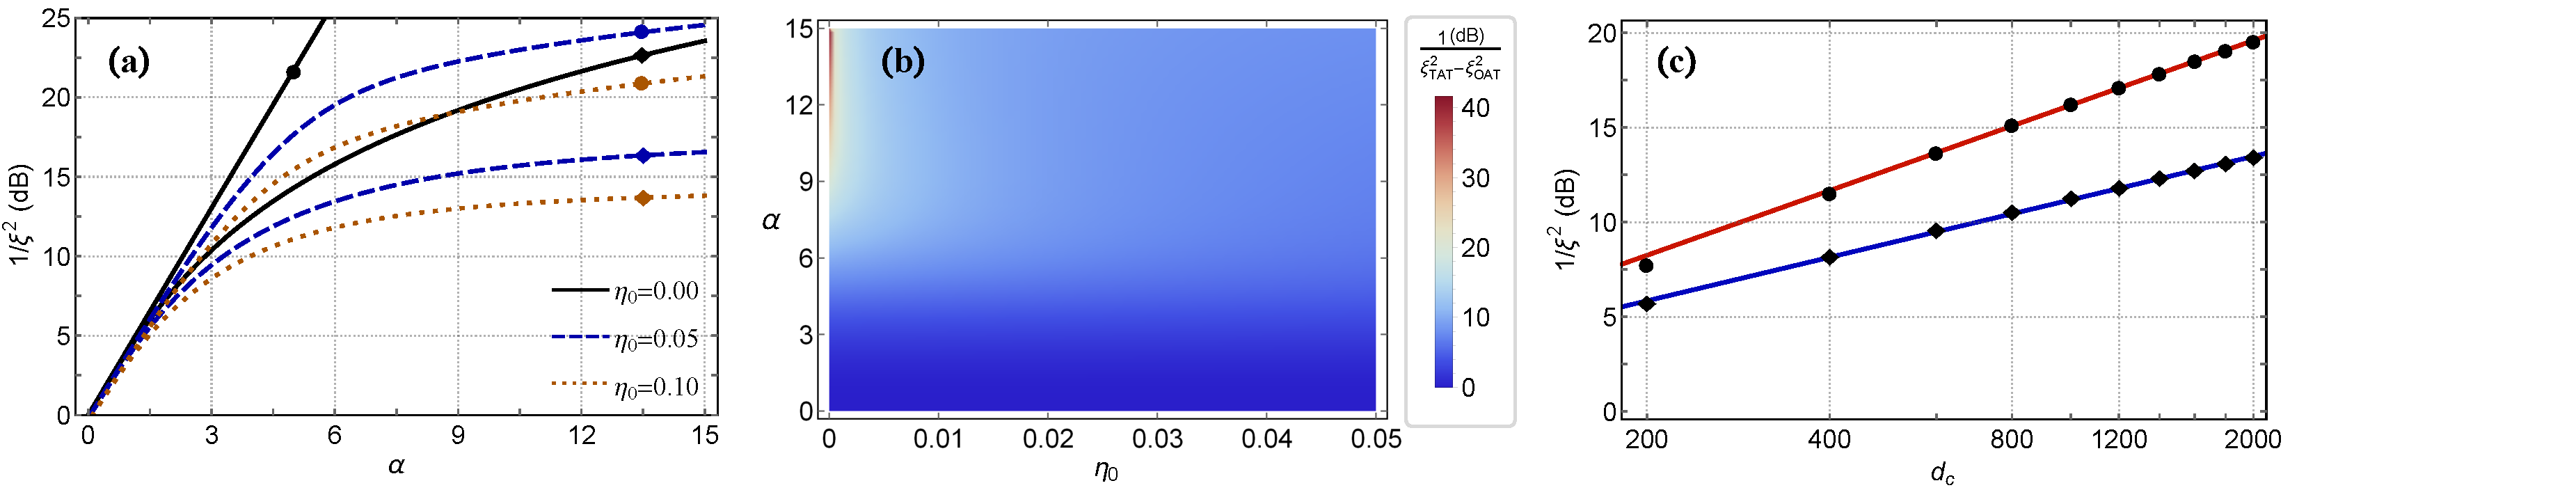
\includegraphics[scale=0.26]{Img/Fig_2.pdf}
	\bicaption{
		(a)OAT(带有菱形的线)和TAT(带圆圈的线)协议的性能随着各种原子衰变值的耦合强度$ \alpha $而变化的曲线。
		(b)两个方案产生的压缩度之差随耦合强度$ \alpha $和原子衰变$ \eta_0 $的变化。 
		(c)为$r_0 = 0.1$时OAT(钻石线)和TAT(圆圈线)方案随腔OD $d_c$变化的最佳挤压效果。}
	{
		(a) Performance of OAT (lines with diamond) and TAT (lines with circle) protocols varies with coupling strength $\alpha$ for various values of atomic decay. 
		(b) Squeezing difference of the two proposed squeezing protocols versus coupling strength $\alpha$ and atomic decay $\eta_0$. 
		(c) Best achievable squeezing of OAT (line with diamonds) and TAT (line with circles) protocols versus cavity OD dc for $r_0=0.1$.}
		\label{figure42}
\end{figure}

  我们首先计算了压缩参数$\xi^2\simeq2(\Delta\hat{X}_\theta^{out})^2/(1-\eta_0)$并绘制图\ref{figure42},在图(a)中我们绘制了依赖于耦合强度$\alpha$的各种原子衰变值的压缩量。从中可以看出如果原子衰变小于10\%,那么对于相互作用参数$\alpha=5$,可以获得大于10dB的压缩度。此外,正如预期的那样,TAT协议比OAT协议更加有效,即使在有噪音的情况下。对协议性能与原子衰减的进一步研究(如图(b)所示)表明TAT协议对于噪声更加敏感,相反,OAT协议对原子衰变显得更加稳定。因此,对于TAT协议,我们需要极低的衰减率来保留它的优点。在实际实现中,使用可访问的实验参数OD来评估所提议的协议的性能是非常方便的。在图(c)中,我们绘制了两个所提协议相对于腔OD$d_c$的最佳可实现的压缩图像(相对于$\eta_0$优化)。对于自由空间OD大约为30\cite{JPB2008qf}的室温蒸汽,如果设置参数$r_0=0.1$和精细$F\simeq100$,OAT和TAT产生的压缩度将分别达到13.4dB和19.6dB。

  我们对于具体的实验实现也进行了相关的参数估计。我们考虑一个含有$5\times 10^6$个原子的原子样品,并选择一个真实的腔耦合参数$g=(2\pi)100kHz$。如果选择参数$\gamma=\kappa\sim10^2g$,$\Omega\sim10^4g$,$\Delta\sim10^5g$和$\delta\sim5\times10^2g$,取$\alpha\simeq5$,我们将得到相互作用时间$t$大约在$0.3\mu s$左右,在$\eta_0<10\%$,$r_0\ge1$的情况下,最终我们将得到大于10dB的压缩度。
  
\vbox{}
\section{结论}
\vbox{}
  我们提出了一种在光学腔中原子系综产生高度自旋压缩态的方案。该过程基于光和自旋极化原子系综之间的非共振SRS相互作用。通过向放置在最初处于真空态的光学腔中的极化原子蒸汽发送强脉冲,我们发现可以实现OAT压缩。腔场与原子之间的相互作用越强,压缩程度越高。我们还表明,通过沿自旋极化方向添加均匀磁场,可以将OAT协议转换为更有效的TAT协议。我们在不同噪声的影响下对方案进行测试,我们发现如下的特点:

    (1)即使在存在大约10\%的原子发生衰减的情况下,我们的体系仍然可以获得大于10dB的压缩;

    (2)尽管TAT协议的性能一般来说要比OAT协议更有优异,但是其对于原子的衰减却更加敏感;

    (3)OAT协议在对抗噪声的影响方面显得叫TAT协议更加强大。

  因此,我们认为尽管OAT协议在压缩方面并不优于TAT协议,但它在嘈杂的环境中易于存活的良好特性以及更简单的实验设置使其适用于各种原子系统。我们期望所提出的协议在量子信息处理和量子计量的背景下是有益的。





\chapter{在光学腔中利用相干光场制备原子系综的纠缠态}\label{chapter4}
\vbox{}\vbox{}
原子系综的纠缠在量子信息处理与量子精密测量中有着重要的应用,其是实现远距离量子通信、构建高效量子存储器的基础。本文提出了一种简单但易于实验实现的理论方案用以制备原子系综间的纠缠,即通过向光学腔中注入相干(经典)光场,以相干光场为驱动力,同时利用腔模的量子输运效应实现两个原子系综之间的高斯纠缠。我们发现本方案所产生的纠缠根植于量子非破坏性测量相互作用,而这一类型相互作用在连续变量计算中有也有着很重要的应用。

\vbox{}
\section{引言}
\vbox{}
量子纠缠是量子力学中许多问题的核心\cite{bouwmeester2000physics,horodecki2009quantum,knill2005quantum},近年来正在引起越来越多的关注。在若干量子信息\cite{bennett1993teleporting,bennett1992communication,beige2001secure}处理问题中都需要用到纠缠,例如在量子远程传送\cite{pirandola2015advances,herbst2017quantum}和量子通信\cite{gisin2007quantum,ursin2007entanglement}以及在某些量子加密协议中\cite{broadbent2019uncloneable,yang2018mutual}都需要用到它。它在量子计算\cite{maezawa2018toward,grover1996fast}中也发挥着重要作用,使得量子计算机可以在诸如素数因子分解或搜索\cite{nielsen2002quantum,ekert1996quantum,vandersypen2001experimental}等几个问题上超越经典计算机。此外,在研究量子力学中的某些非经典现象时,量子纠缠的产生也成为当今量子调控实现的目标。

原子系综作为量子纠缠的载体,因为其具备易于实现与弱光场的相互作用以及抵御体系退相干等诸多优点而正引起研究者的极大兴趣。迄今为止,已有多种方案被提出用于制备原子系综的纠缠态。其中一种方法是光场记忆法\cite{lukin2000entanglement},即通过将纠缠光场分别存储到两个原子系综用以建立原子间的纠缠;另外一种方法是投影测量法\cite{duan2000quantum},即首先建立光与原子间的纠缠,而后对出射光场做投影测量即可实现体系的纠缠交换,从而实现原子与原子间的纠缠。对于光场记忆法,显然原子系综的纠缠度受制于光场的纠缠度以及光记忆的保真度;而对于投影测量法体系的纠缠度受制于探测器的探测效率。本文提出了一种不同此两种的新方法,即将原子系综放置于光学腔中,通过相干光场驱动,利用腔模的“量子公共汽车”效应建立起原子之间的非经典关联。与之前的方法相比,我们的方案即不需要非经典的量子资源,也不需要高效的量子态探测技术,故可极大地简化实验实施过程,提高纠缠产生的效率。

我们所研究的量子系统是由大量原子自旋组成的原子系综,对于由N个自旋1/2粒子的系统,我们可定义可观察量的集体角动量算符
\begin{align}\label{eq551}
	{J_l} = \frac{1}{2}\sum\limits_{k = 1}^N {\sigma _l^{(k)}} ,
\end{align}
其中$l=x,y,z$,$\sigma_l^{k}$是Pauli矩阵。三个正交方向上的自旋分量之间满足对易关系$[J_x,J_y]=i\hbar J_z$,这里的${J_x} = ({J_ + } + {J_ - })/2$和${J_y} = ({J_ + } - {J_ - })/2i$,其中$J_+(J_-)$表示原子的升(降)算符。如果系综里的所有原子朝着$x$方向极化,则我们可利用Holstein-Primakoff近似\cite{zhang1998even}将轨道角动量振子化,即可定义新的原子量子变量${X_a} = {J_y}/\sqrt {{J_x}} $,${P_a} = {J_z}/\sqrt {{J_x}} $,满足 $[ X_a, P_a] = i$。对于CSS,有$\braket{ X_a}=\braket{ P_a} = 0$和归一化方差${(\Delta {X_a})^2} = {(\Delta { P_a})^2} = 1/2$。
于是,原子系综间的纠缠问题转化为振子间的连续变量纠缠问题。本文的结构主要如下:在第二部分我们首先并给出了两个原子系综之间产生纠缠的详细过程,并对产生的纠缠进行了判据;第三部分我们简要分析了噪声对纠缠的影响;第四部分是结论的和分析。
\begin{figure}[htbp]
	\centering
	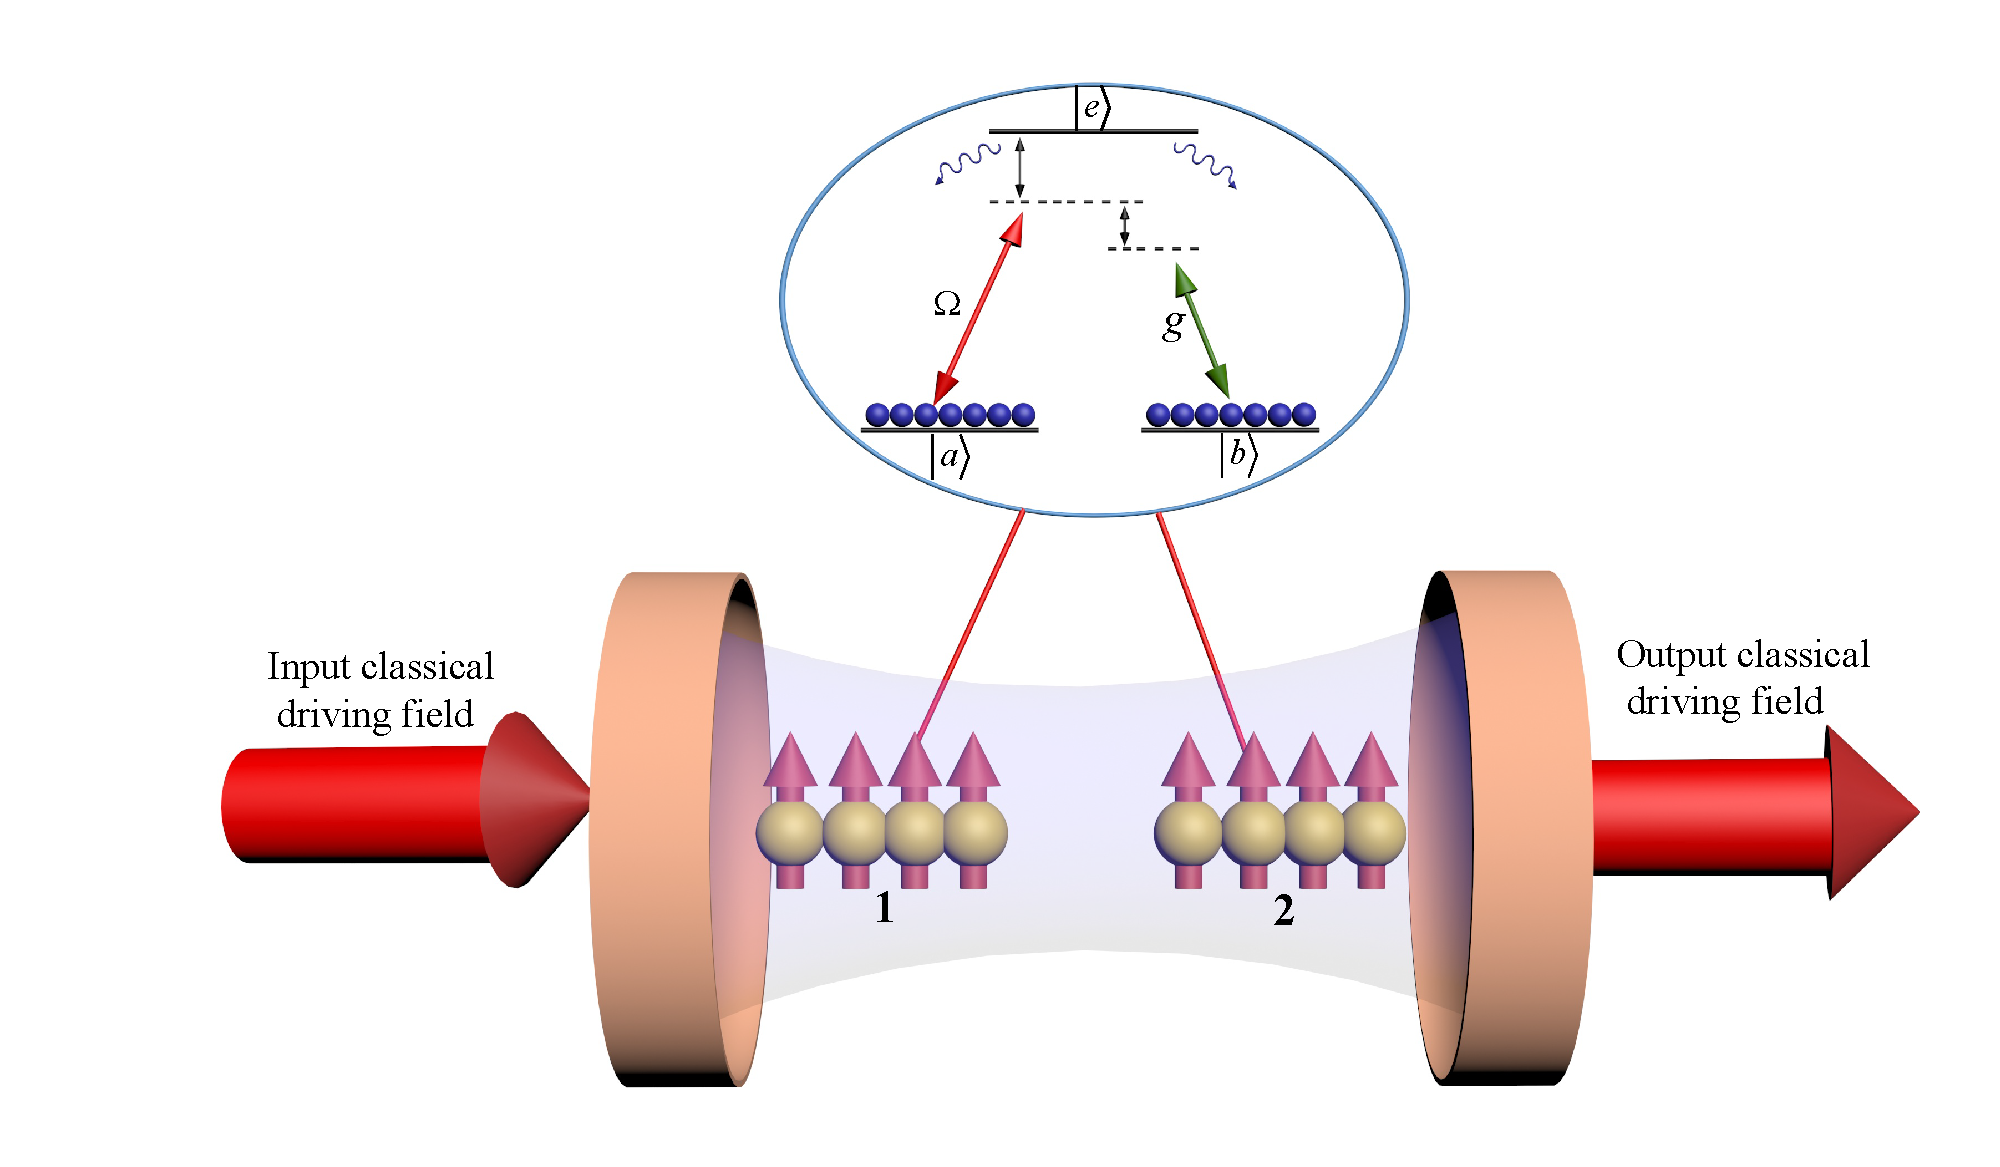
\includegraphics[scale=0.35]{Img/Fig_551.pdf}
	\bicaption{$\Lambda$型的原子系综和腔场的耦合示意图。一束激光与两原子系综的基态$\ket{a}$和激发态$\ket{e}$实现非共振耦合,而基态$\ket{b}$和激发态$\ket{e}$与处于真空态的腔模相耦合,绝热消除原子的激发态与腔模后即可得到原子的等效演化,该演化正是原子间纠缠产生的根源。}	
	{Schematic diagram of the $\Lambda$-type atomic ensemble coupling with cavity field. A laser beam couples off-resonantly with two atomic ensembles by the ground state $\ket{a}$ and the excited state $\ket{e}$, while the ground state $\ket{b}$ and the excited state $\ket{e}$ are coupled with the cavity mode in the vacuum state. By adiabatic elimination of the atom excited state and the cavity mode, one obtains and effective evolution of atoms, which is the source of entanglement between atoms.}
	\label{figure51}
\end{figure}

\vbox{}
\section{纠缠态的产生}
\vbox{}
考虑有两个完全相同的$\Lambda$型的三能级原子系综置于单模腔场中并与腔场相互作用的模型,其原子数分别为$N_1$和$N_2$,能级结构示意图如图\ref{figure51}所示。原子有两个稳定的基态$\ket{a}$、$\ket{b}$和激发态$\ket{e}$,两个基态之间的能级差是$\omega_{ab}$(这里我们取$\hbar=1$),基态$\ket{a}$和激发态$\ket{e}$之间的能级差是$\omega_{ae}$。基态$\ket{a}$和激发态$\ket{e}$之间通过一个频率为$\omega$经典驱动场相耦合,其共振拉比频率为$\Omega$,与基态$\ket{b}$之间的耦合则通过与腔模$c$的相互作用来完成。

对于这两个三能级原子系综与单模腔场相互作用的系统,我们可以很容易的写出系统的哈密顿量为
\begin{align}\label{eq552}
	\begin{split}
		\hat H   =& \omega_0\hat c^\dag \hat c+\sum_{i}^{2}[\sum_k \omega_{ae}\ket{e}_k\bra{e}
		+ H_I]_i \\
		&H_I= \sum_k (\frac{\Omega}{2}e^{-i\omega t}\ket{e}_k\bra{a}
		+g\hat c\ket{e}_k\bra{b}+h.c.),
	\end{split}
\end{align}
其中$\hat c$和$\hat c^\dagger$表示光场的湮灭和产生算符,$\omega_0$是相应腔模的频率,$g$是原子与腔场的耦合常数,下标1和2分别表示1和2号原子系综的算符,$\sum_i^2$表示对两个原子系综的哈密顿量求和。

接下来我们令$\hat \sigma_{\mu\nu}=\sum_k{\ket{\mu}_k\bra{\nu}}$(其中$\mu,\nu\in {1,2,3}$)对公式(\ref{eq552})中的哈密顿量进行化简,则有
\begin{align}\label{eq553}
	\begin{split}
		\hat H   = \omega_0\hat c^\dag \hat c + \omega_{ae}\sigma_{ee}
		+(\frac{\Omega}{2}e^{-i\omega t}\sigma_{ea}+g\hat c\sigma_{eb}+h.c.),
	\end{split}
\end{align}
其中我们定义了算符
\begin{align}	\label{eq554}
	\begin{split}
		\omega_{ae}\sigma_{ee}                   &= (\omega_{ae}\sigma_{ee})_1
		+(\omega_{ae}\sigma_{ee})_2,\\
		\frac{\Omega}{2}e^{-i\omega t}\sigma_{ea}&= (\frac{\Omega}{2}e^{-i\omega t}\sigma_{ea})_1
		+(\frac{\Omega}{2}e^{-i\omega t}\sigma_{ea})_2,\\
		g\hat c\sigma_{eb}                       &= (g\hat c\sigma_{eb})_1
		+(g\hat c\sigma_{eb})_2,
	\end{split}
\end{align}
通过上式我们可以看到,两个小原子系统的总哈密顿量可以写成一个大原子系综的哈密顿量。我们也可以很容易的写出$J_l=J_{l1}+J_{l2}$,其中$l=x,y,z$。

接下来我们进入一个转动坐标系,这一转动由哈密量$\hat H_0^1= \omega_0\hat c^\dag \hat c + \omega_{ae}\sigma_{ee}$来统治,对公式\ref{eq553}的哈密顿量进行旋转后,得到
\begin{align}\label{eq555}
	\begin{split}
		\hat{ H}_{eff}^1 &= {e^{i{{\hat H}_0}t/\hbar }}\hat H{e^{ - i{{\hat H}_0}t/\hbar }} 
		- {{\hat H}_0}\\
		&= \Delta {{\hat \sigma }_{33}} + \frac{\Omega }{2}{{\hat \sigma }_{31} }
		+ g\hat \varepsilon {{\hat \sigma }_{32}} 
		+ \frac{{{\Omega ^*}}}{2}{{\hat \sigma }_{13}}
		+ g{{\hat \sigma }_{23}}{{\hat \varepsilon }^\dag },
	\end{split}
\end{align}
式中我们定义了一个新算符$\hat \varepsilon  = \hat c{e^{i\delta t}}$。根据哈密顿量,我们可以计算出光和原子的海森堡方程,得到如下的Maxwell-Bloch方程
\begin{align}\label{eq556}
	\begin{split}
		{\dot{\hat{ \sigma}} _{11}}  & =  i\frac{\Omega }{2}{\hat \sigma _{31}} 
		- i\frac{{{\Omega ^*}}}{2}{\hat \sigma _{13}},\\
		{\dot {\hat{ \sigma}} _{22}} & =  ig\hat \varepsilon {\hat \sigma _{32}} 
		- i{g^*}{\hat \sigma _{23}}{\hat \varepsilon ^\dag },\\
		{\dot {\hat{ \sigma}} _{12}} & =  i\frac{\Omega }{2}{\hat \sigma _{32}} 
		- i{g^*}{\hat \sigma _{13}}{\hat \varepsilon ^\dag },\\
		{\dot {\hat{ \sigma}} _{13}} & =- i\Delta {\hat \sigma _{13}} 
		- i\frac{\Omega }{2}\left( {{{\hat \sigma }_{11}} - {{\hat \sigma }_{33}}} \right) - ig\hat \varepsilon {\hat \sigma _{12}},\\
		{\dot {\hat{ \sigma}} _{23}} & =- i\Delta {\hat \sigma _{23}}-i\frac{\Omega }{2}{\hat \sigma _{21}}
		- ig\hat \varepsilon \left( {{{\hat \sigma }_{22}} 
			- {{\hat \sigma }_{33}}} \right),\\
		{\dot {\hat{ \sigma}} _{33}} & =  i\frac{{{\Omega ^{\rm{*}}}}}{2}{\hat \sigma _{13}}
		- i\frac{\Omega }{2}{\hat \sigma _{31}} 
		+ i{g^{\rm{*}}}{\hat \sigma _{23}}{\hat \varepsilon ^ + } 
		- ig\hat \varepsilon {\hat \sigma _{32}},\\
		\dot {\hat{ \varepsilon}}    & =- i{g^*}{\hat \sigma _{23}} + i\delta \hat \varepsilon , 
	\end{split}
\end{align}
接下来,为了方便计算,我们做如下的假设:1.假设经典驱动场足够的弱。2.假设失谐量$\Delta\gg 1$。通过这样的假设,可以认为布居在激发态的原子数非常少,因此可以绝热消除掉激发态(${\sigma _{33}} \simeq 0$)。大失谐还可以将$\sigma_{13}$和$\sigma_{23}$快速驱动到稳态,于是有${\hat \sigma _{13}} \simeq  - \left( {\Omega {{\hat \sigma }_{11}}/2 + g\hat \varepsilon {{\hat \sigma }_{12}}} \right)/\Delta $,${\hat \sigma _{23}} \simeq  - \left( {\Omega {{\hat \sigma }_{21}}/2 + g\hat \varepsilon {{\hat \sigma }_{22}}} \right)/\Delta $ 。我们进一步假设双光子失谐量足够大$\delta\gg 1$,使得在相互作用期间腔中没有产生显着的光子激发,这使得能够绝热地消除腔场,导致$\hat \varepsilon  =  - {g^*}\Omega {\hat \sigma _{21}}/2\Delta \delta $。基于这些假设,原子的基态方程可以写为
\begin{align}
	{\dot{ \hat{ \sigma}} _{12}} =  - i{\kappa _0}{\hat S_z}{{ \hat{ \sigma}} _{12}}
	- i{\chi _0}{{ \hat{ \sigma}} _{12}},{\dot { \hat{ \sigma}} _{11}} = {\dot { \hat{ \sigma}} _{22}} = 0,\label{eq557}
\end{align}
其中定义了$\kappa_0=|\Omega|^2{|g|^2}/4{\delta\Delta^2}$ 和 $\chi_0 ={|\Omega|^2}/{4\Delta}$。在伪角动量运算符的表述中,公式(\ref{eq557})可以写为
\begin{align}\label{eq558}
	\begin{split}
		{{\dot {\hat J}}_x} &=  {\kappa _0}\left( {{{\hat J}_y}{{\hat J}_z} 
			+ {{\hat J}_z}{{\hat J}_y}} +{{\hat J}_y}\right) 
		+ {\chi _0}{{\hat J}_y},\\
		{{\dot {\hat J}}_y} &=- {\kappa _0}\left( {{{\hat J}_x}{{\hat J}_z} 
			+ {{\hat J}_z}{{\hat J}_x}} +{{\hat J}_x}\right) 
		- {\chi _0}{{\hat J}_x},\\
		{{\dot {\hat J}}_z} &= 0,
	\end{split}
\end{align}
从上面的这组方程,可以推断原子的动力学是由下式的有效哈密顿量产生的
\begin{align}
	\hat H_{eff}^2=-\chi_0\hat S_z-\kappa_0(\hat S_z+\hat S_z^2),
	\label{eq559}
\end{align}
从哈密顿量的形式我们知道这是一个OAT型的哈密顿量\cite{PRA1993Kitagawa}。(\ref{eq559})式的第一项出现源于基态的AC-Stark平移,而其余项源于双光子非共振拉曼跃迁。通过取参数$\chi_0=-\kappa_0$,公式(\ref{eq559})中的有效哈密顿量将变成一个纯粹的OAT哈密顿量,即$\hat H_{eff}=\chi_0 S_z^2$。

将系统总的自旋用两个小系综的自旋之和来表示,于是我们可以将系统的哈密顿量重新写为如下的形式,
\begin{align}\label{eq5510}
	\begin{split}
		\hat H_{eff}^3& = {\chi _0}J_z^2\\
		&= {\chi _0}{({J_{z1}} + {J_{z2}})^2}\\
		&= {\chi _0}(J_{z1}^2 + J_{z2}^2 + 2{J_{z1}}{J_{z2}}),
	\end{split}
\end{align}
然后我们进入$\hat H_0^2 = J_{z1}^2 + J_{z2}^2$的转动坐标系,可以得到在新的相互作用绘景下有效哈密顿量
\begin{align}\label{eq5511}
	\begin{split}
		\hat{H}_{eff}=\chi\hat{P}_1\hat{P}_2,
	\end{split}
\end{align}
其中我们定义了$\chi=2\chi_0 \sqrt{J_{x1}J_{x2}}$。我们也定义了原子系综的动量位置算符$\left( {{{\hat X}_1},{{\hat P}_1}} \right)$和$\left( {{{\hat X}_2},{{\hat P}_2}} \right)$,其满足对易关系$\left[ {{{\hat X}_1},{{\hat P}_1}} \right] = \left[ {{{\hat X}_2},{{\hat P}_2}} \right] = i$,且有$\left\langle {{{\hat X}_1}} \right\rangle  = \left\langle {{{\hat X}_2}} \right\rangle  = \left\langle {{{\hat P}_1}} \right\rangle  = \left\langle {{{\hat P}_2}} \right\rangle  = 0$,$\left\langle {\hat X_1^2} \right\rangle  = \left\langle {\hat X_2^2} \right\rangle  = \left\langle {\hat P_1^2} \right\rangle  = \left\langle {\hat P_2^2} \right\rangle  = \frac{1}{2}$。接下来我们将证明在这个哈密顿量的作用下,两个原子系综之间存在着量子纠缠。

我们首先可以利用公式(\ref{eq5511})中给出的哈密顿量,计算出原子算符随时间的演化方程
\begin{align}\label{eq5512}
	{{\dot {\hat{ X}}}_1} = \chi {{\hat P}_2},
	{{\dot {\hat{ P}}}_1} = 0 ,
	{{\dot {\hat{ X}}}_2} = \chi {{\hat P}_1},
	{{\dot {\hat{ P}}}_2} = 0,
\end{align}
通过求解方程(\ref{eq5512}),我们得到
\begin{align}\label{eq5513}
	\left( {\begin{array}{*{20}{c}}
			{\hat X_1^{out}}\\
			{\hat P_1^{out}}\\
			{\hat X_2^{out}}\\
			{\hat P_2^{out}}
	\end{array}} \right) = \left( {\begin{array}{*{20}{c}}
			1   & 0     & 0   & \kappa\\
			0   & 1     & 0   & 0     \\
			0   &\kappa & 1   & 0     \\
			0   & 0     & 0   & 1
	\end{array}} \right)\left( {\begin{array}{*{20}{c}}
			{\hat X_1^{in}}\\
			{\hat P_1^{in}}\\
			{\hat X_2^{in}}\\
			{\hat P_2^{in}}
	\end{array}} \right)
\end{align}

其中$\kappa=\chi t$,“in”表示最初系统演化之前的量子态,“out”表示系统演化之后输出的量子态。

很显然,我们这里原子系综的量子态是高斯态,因为初始输入态是真空态,而相互作用的哈密顿量是正则算符平方,故相互作用过程不改变体系量子态的高斯特性\cite{simon2000peres},于是我们可以很方便的用Wigner函数来表示体系的量子态,即可得到
\begin{align}\label{eq5514}
	W(\xi)=\frac{1}{(2\pi)\sqrt{det V^{(2)}}}exp^{{-\frac12\xi[V^{(2)}]^{-1}\xi^T}},
\end{align}
这里$\xi = [{X_1},{P_1},{X_2},{P_2}]$是正则矢量算符,V是关联矩阵,关联矩阵的矩阵元计算方法如下所示\cite{braunstein2005quantum}
\begin{align}\label{eq5515}
	V_{ij}=\braket{(\hat{\xi}_i\hat{\xi}_j+\hat{\xi}_j\hat{\xi}_i)/2},
\end{align}
对于方程(\ref{eq5514})中的高斯态,Wigner函数完全由二阶关联矩阵确定。对于经典4维相空间上的经典概率分布,每个物理相关矩阵是正的、实数和对称的。与之对应的,任何实的、对称的正矩阵都表示可能的物理关联矩阵。除了正的、实数和对称的之外,描述量子相空间的Wigner相关矩阵(任意态)也必须满足如下的关系
\begin{align}\label{eq5516}
	[\hat{\xi}_k,\hat{\xi}_l]=\frac{i}{2}\Lambda_{k,l},k,l=1,2,3,4
\end{align}
对于4×4矩阵$\Lambda$,其具有2×2矩阵J作为每个正交对的对角项
\begin{align}\label{eq5517}
	\Lambda=\left( {\begin{array}{*{20}{cc}}
			J  & 0\\
			0  & J
	\end{array}} \right)
	,J=\left( {\begin{array}{*{20}{cc}}
			0  & 1\\
			-1 & 0
	\end{array}} \right).
\end{align}

现在让我们考虑任意双模态。根据公式(\ref{eq5515})中的双模关联矩阵$V^(2)$的定义,我们可以以分块的形式写出任意双模态的关联矩阵
\begin{align}\label{eq5518}
	V=\left( {\begin{array}{*{20}{cc}}
			A  & C\\
			C^T& B
	\end{array}} \right)
\end{align}
其中A,B和C是实的2×2的矩阵。Simon的Peres-Horodecki判据如下
\begin{align}\label{eq5519}
	\begin{split}
		F=\det{A}\det{B}+(\frac1{16}-|\det{C}|)^2&-Tr(AJCJBJC^TJ)\\
		&\ge G=\frac1{16}(\det{A}+\det{B}),
	\end{split}
\end{align}
其中J是公式(\ref{eq5517})中的2×2矩阵。任意的可分离的两高斯模满足不等式$F\ge G$,它代表了可分离性的必要条件,因此它的违反是不可分离性的充分条件。

利用前面公式(\ref{eq5515})给出的表达式,我们可以计算两原子系综与光场相互作用系统的关联矩阵,于是有
\begin{align}\label{eq5520}
	{V_{ij}} =\frac14 \left( 
	{
		\begin{array}{*{20}{c}}
			1+\kappa^2 &    0   &    0       & \kappa \\
			0      &    1   & \kappa     &    0   \\
			0      & \kappa & 1+\kappa^2 &    0   \\
			\kappa   &    0   &    0       &    1
		\end{array}
	} 
	\right),
\end{align}
接下来我们可以将$V_{ij}$方块化,得到
\begin{align}\label{eq5521}
	A=\left(
	{
		\begin{array}{*{20}{cc}}
			1+\kappa^2  & 0\\
			0        & 1
		\end{array}
	} 
	\right),
	B=\left(
	{
		\begin{array}{*{20}{cc}}
			1+\kappa^2  & 0\\
			0        & 1
		\end{array}
	} 
	\right),
	C=C^T=\left(
	{
		\begin{array}{*{20}{cc}}
			0       & \kappa\\
			\kappa     &   0 
		\end{array}
	} 
	\right),
\end{align}

我们将公式(\ref{eq5517})中的矩阵J和(\ref{eq5521})中的矩阵A,B,C代入判据公式(\ref{eq5519})中,于是我们将得到如下的结果
\begin{align}\label{eq5522}
	F-G=-\frac1{64}\kappa^2,
\end{align}

很显然,对于任意的$\kappa\ne 0$,两个原子系综之间是相互纠缠的,$\kappa$越大,偏离负值也越大,侧面反映了相互之间的纠缠度也越高,这正是本文的主要结论。

\vbox{}
\section{噪声对方案的影响}
\vbox{}
由于原子的激发态存在着自发辐射,而这些自发辐射会引起原子系综轨道角动量的等效退相干,于是我们可以得到新的正则算符的演化方程\cite{liu2018spin}
\begin{align}\label{eq5523}
	\begin{split}
		{\dot{ \hat X}_1} &= \chi {{\hat P}_2} - \eta {{\hat X}_1} + \sqrt {2\eta } {\hat F}_{{X_1}},\\
		{\dot{ \hat P}_1} &=  - \eta {{\hat P}_1} + \sqrt {2\eta } {{\hat F}_{{P_1}}},\\
		{\dot {\hat X}_2} &= \chi {{\hat P}_1} - \eta {{\hat X}_2} + \sqrt {2\eta } {\hat F}_{{X_2}},\\
		{\dot {\hat P}_2} &=  - \eta {{\hat P}_2} + \sqrt {2\eta } {{\hat F}_{{P_2}}},
	\end{split}
\end{align}
这里$\eta=\chi_0 \gamma/\Delta$是光的泵浦率,其中$\gamma$表示原子激发态到基态的自发辐射系数。${\hat F_{{X_1}}},{\hat F_{{P_1}}}{\rm{, }}{\hat F_{{X_2}}}{\rm{, }}{\hat F_{{P_2}}}$是朗之万噪声项,它们满足对易关系$\left[ {{{\hat F}_{{X_1}}},{{\hat F}_{{P_1}}}} \right]{\rm{ = }}\left[ {{{\hat F}_{{X_2}}}{\rm{, }}{{\hat F}_{{P_2}}}} \right] = i$。根据方程(\ref{eq5523})我们可以得到新的输入输出关系
\begin{align}\label{eq5524}
	\begin{split}
		\hat X_1^{out} =& {e^{ - \eta t}}\hat X_1^{in} 
		+ \sqrt {2\eta } {e^{ - \eta t}}\int_0^t {{e^{\eta \tau }}{{\hat F}_{{X_1}}}d\tau  
			+ \chi {e^{ - \eta t}}\int_0^t {\hat P_2^{in}d\tau } } \\
		&+ 2\eta \chi {e^{ - \eta t}}\int_0^t {(t - \tau ){e^{\eta \tau }}{{\hat F}_{{P_2}}}d\tau } ,\\
		\hat P_1^{out} =& {e^{ - \eta t}}\hat P_1^{in} 
		+ \sqrt {2\eta } {e^{ - \eta t}}\int_0^t {{e^{\eta \tau }}{{\hat F}_{{P_1}}}d\tau ,} \\
		\hat X_2^{out} =& {e^{ - \eta t}}\hat X_2^{in} 
		+ \sqrt {2\eta } {e^{ - \eta t}}\int_0^t {{e^{\eta \tau }}{{\hat F}_{{X_2}}}d\tau  
			+ \chi {e^{ - \eta t}}\int_0^t {\hat P_1^{in}d\tau } } \\
		&+ 2\eta \chi {e^{ - \eta t}}\int_0^t {(t - \tau ){e^{\eta \tau }}{{\hat F}_{{P_1}}}d\tau } ,\\
		\hat P_2^{out} =& {e^{ - \eta t}}\hat P_2^{in} 
		+ \sqrt {2\eta } {e^{ - \eta t}}\int_0^t {{e^{\eta \tau }}{{\hat F}_{{P_2}}}d\tau } ,
	\end{split}
\end{align}
利用公式(\ref{eq5524})的结果,通过公式(\ref{eq5515})我们可以计算得出系统在存在噪声的情况下的关联矩阵为 
\begin{align}\label{eq5525}
	{V_{ij}} =\frac14 \left( 
	{
		\begin{array}{*{20}{c}}
			1+\kappa^2 - 2\kappa^2\tilde \eta &    0   &    0       & \kappa- 2\kappa\tilde \eta \\
			0      &    1   & \kappa- 2\kappa\tilde \eta     &    0   \\
			0      & \kappa- 2\kappa\tilde \eta & 1+\kappa^2- 2\kappa^2\tilde \eta &    0   \\
			\kappa- 2\kappa\tilde \eta   &    0   &    0       &    1
		\end{array}
	} 
	\right),
\end{align}
其中我们重新定义了$\tilde \eta  = \eta t$。于是我们得到一组新的分块矩阵
\begin{align}\label{eq5526}
	A&=\left(
	{
		\begin{array}{*{20}{cc}}
			1+\kappa^2 - 2\kappa^2\tilde \eta  & 0\\
			0        & 1
		\end{array}
	} 
	\right),
	B=\left(
	{
		\begin{array}{*{20}{cc}}
			1+\kappa^2 - 2\kappa^2\tilde \eta  & 0\\
			0        & 1
		\end{array}
	} 
	\right),\\
	C&=C^T=\left(
	{
		\begin{array}{*{20}{cc}}
			0       & \kappa- 2\kappa\tilde \eta\\
			\kappa- 2\kappa\tilde \eta     &   0 
		\end{array}
	} 
	\right).
\end{align}

接下来我们将利用新计算得出的矩阵A,B,C以及公式(\ref{eq5517})中的矩阵J,将它们代入判据公式(\ref{eq5519})重新对系统进行判据已得到在噪声存在的情况下,其对纠缠判据的影响,于是我们得到了如下的结果
\begin{align}\label{eq5527}
	F - G =  - \frac{1}{{64}}{\kappa ^2} + \frac{{\tilde \eta }}{{16}}{\kappa ^2} - \frac{{{{\tilde \eta }^2}}}{{16}}{\kappa ^2} + \frac{{{{\tilde \eta }^2}}}{{64}}{\kappa ^4} - \frac{{{{\tilde \eta }^3}}}{{16}}{\kappa ^4} + \frac{{{{\tilde \eta }^4}}}{{16}}{\kappa ^4},
\end{align}
上式中第一项为纯相互作用的项,其不受噪声的影响,通过令$\tilde \eta  = 0$,即当噪声不存在的情况下,上式将变回(\ref{eq5522})式。
\begin{figure}[htbp]
	\centering
	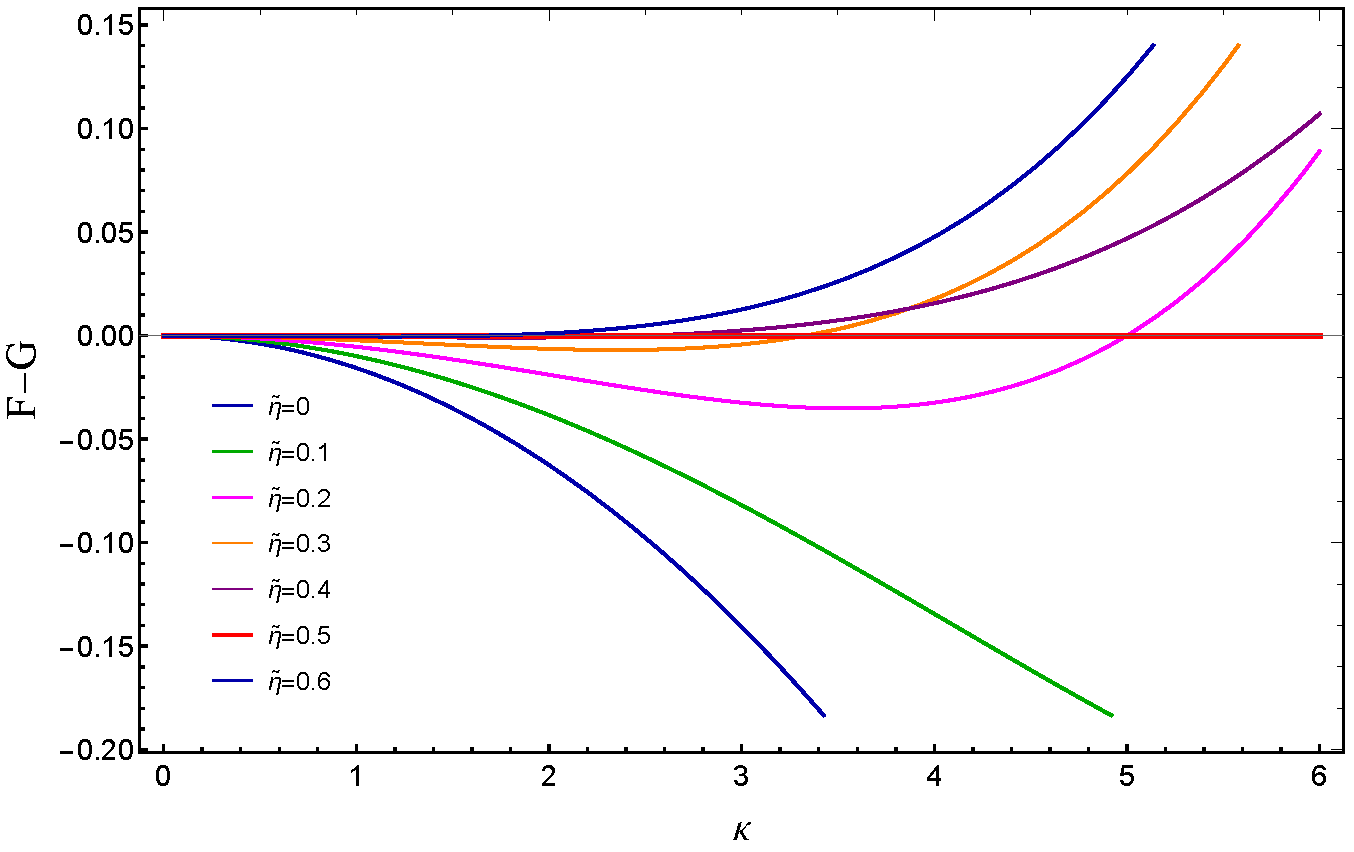
\includegraphics[scale=0.4]{Img/Fig_552.pdf}
	\bicaption{纠缠判据F-G随相互作用强度$\kappa$变化的图像。图中给出了在不同退相干系数$\tilde \eta$的影响下判据F-G随$\kappa$变化的曲线。}{A plot of the F-G as a function of the coupling strength $\kappa$. The figure shows a variation of the criterion F-G with coupling strength $\kappa$ under different decay rate $\tilde \eta$.}	
	\label{figure552}
\end{figure}


图\ref{figure552}所示是判据F-G随相互作用强度$\kappa$变化的曲线,从图中我们可以得出以下结论:(1)当$\tilde \eta  = 0$时(图中黑线),曲线随着$\kappa$越来越大,偏离负值的也在逐渐变大,侧面反映了相互之间的纠缠度随着$\kappa$的增大而增大。(2)当$0 < \tilde \eta  < 0.5$时,曲线随着$\kappa$值的增大偏离负值会先增大而后减小,表示由于噪声的影响,随着相互作用强度的增大,纠缠度不会一直增加,在其到达一个峰值以后反而会减小。(3)当$\tilde \eta  = 0.5$时,曲线完全与横轴重合,且不随$\kappa$而变化。(4)当$\tilde \eta  > 0.5$时,曲线始终在横轴上方,且会随着$\kappa$的增大偏离正值也越大,表明当噪声影响很大的时候,原子的相干演化完全为体系的噪声所淹没。以上就是我们得到的主要结论,我们发现,在存在噪声的情况下,相互作用强度并不是越大越好,而是有一个最佳值,超过这个值,纠缠度反而会随着相互作用强度的增大而减小。


\vbox{}
\section{结论}
\vbox{}
我们研究了在光学腔中的两个原子系综的纠缠问题,通过向光学腔中注入相干(经典)光场,以相干光场为驱动力,同时利用腔模的量子输运效应实现两个原子系综之间的高斯纠缠。通过结果分析我们发现本方案可以很好地产生两个原子系综之间的量子纠缠,而所产生的这种纠缠根植于原子间量子非破坏性测量相互作用。故而我们相信本方案所产生的原子不仅在诸如量子通信与量子存储方面有着重要的应用,在连续变量计算中也有着潜在的应用。我们期望我们的方案可以对量子信息的发展起到积极的作用。










%
\chapter{结论与展望}\label{chapter5}
\vbox{}\vbox{}
\section{结论}
  量子纠缠是一种很宝贵的资源,可以用来验证量子力学中的基本问题,在量子信息中也有很重要的应用。它和自旋压缩作为量子信息处理的基本资源,在量子光学领域占有很重要的地位。
  原子的自旋压缩的应用极为广泛,不光可以用来产生多体纠缠,在精密测量和量子信息的存储等方面也有着很重要的应用。  
  本文主要研究了$\Lambda$型三能级原子在单模光场的驱动下原子系综的自旋压缩特性和两个原子系综之间的纠缠特性。
  
  首先我们研究了光学腔中原子系综的自旋压缩特性,通过分析这些压缩特性我们发现其是单轴扭曲型的压缩,附加适当的磁场可以将单轴扭曲的哈密顿量转变成双轴扭曲的哈密顿量,从而可以提高系统的压缩度。我们还分析了噪声对系统的影响,发现即便在存在噪声的情况下,系统也可以产生很高的压缩度。
  
  然后我们研究了在光学腔中如何建立两个原子系综之间的纠缠的问题,在同一光学腔内放入两个原子系综,通过研究表明这两个系综会在强驱动场的作用下彼此之间建立纠缠。这一纠缠根植于原子之间的非破坏性相互作用,利用Simon的Peres-Horodecki判据证明了在这个哈密顿量下,两个原子系综之间的确存在着非经典关联。我们也研究了噪声对纠缠的影响,研究表明在不存在噪声的影响下,系统的纠缠随着相互作用的强度的增大而逐渐增强。当噪声大于1/2以后,原子之间的纠缠完全被系统的噪声所淹没。而当噪声在0和0.5之间的时候,纠缠由于噪声的影响会先变大后减小。
  
\vspace{0.5cm}
  \section{展望}
  量子信息科学目前正在进行着飞速的发展,关于纠缠和自旋压缩的研究目前也有很多,都取得很不错的成果,部分成果都已经被用到了实际的生活中,但是由于退相干的影响,实际的效果虽然较经典理论的应用有了很大的进步,但是其发展空间依旧还很大。如何实现多量子比特的纠缠和如何有效的克服系统的噪声来实现更高效的压缩这是人们目前致力于攻克的两个难题。

  在原子系综的压缩方面,迄今为止研究的焦点都主要是集中在如何增强原子间的纠缠上,而忽视了原子本身实际上也是一个小系综(例如铯原子的F=4态可等效8个1/2自旋原子),显然,构建原子间纠缠的同时压缩原子内态(即单个原子形成的小系综),必然会增大体系整体的压缩度。如果我们研究对内外态同时作用不同的哈密顿量,观测体系压缩度增加的情况,预计在内外态同时进行压缩的情况下,体系的压缩度将得到大大的提高。与此同时如果我们可以建立一个超真空的环境,在这个环境下对体系进行相应的操作,也许体系受到的环境等其他因素带来的噪声可以大大的降低。
  
    
%\input{Tex/Chap_6}
%---------------------------------------------------------------------------%
% main content
%-
%-> Appendix
%-
%\cleardoublepage%
%\appendix% initialize the environment
%
\chapter[附录]{附录\quad 噪声情况下运动方程的详细推导}\label{appendix}
\vbox{}
\vbox{}
在这个附录中,我们分析了在自发辐射和空腔衰变情况下我们的方案的性能。通过考虑噪音的影响,公式(\ref{eq444})-(\ref{eq4410})的Maxwell-Bloch方程将变为\cite{PhysRevA.76.033804}
\begin{align} \label{a1}
	\begin{split}
\dot {\hat \sigma}_{11}  =& -\Omega_0 \hat S_y + i   \frac \Omega2{ \hat \sigma}_{31} - i \frac{ \Omega^\ast}{2}{ \hat \sigma}_{13} + \gamma{ \hat \sigma}_{33}+ F_{11},\\
\dot {\hat \sigma}_{22} =&~\Omega_0 \hat S_y + i g \hat \varepsilon{ \hat \sigma}_{32} - ig^\ast{ \hat \sigma}_{23} \hat \varepsilon^\dag + \gamma{ \hat \sigma}_{33}+ F_{22},\\
\dot {\hat \sigma}_{12} =& ~ i  \Omega_0  \hat S_z + i   \frac{\Omega}{2}{ \hat \sigma}_{32} - ig^\ast{ \hat \sigma}_{13} \hat \varepsilon^\dag,\\
\dot {\hat\varepsilon} =& - \frac\kappa2\hat\varepsilon - ig^\ast{\hat\sigma}_{23} + \sqrt\kappa{\hat\varepsilon}_{in}+i\delta\hat\varepsilon,\\
\dot {\hat \sigma}_{13} =& -i\frac{ \Omega_0}2 \sigma_{23} - (i  \Delta + \gamma){ \hat \sigma}_{13}-i \frac\Omega2({ \hat \sigma}_{11}-{ \hat \sigma}_{33})\\
&- ig\hat\varepsilon{\hat\sigma}_{12} + F_{13},\\
\dot {\hat \sigma}_{23} =& -i\frac{ \Omega_0}2 \sigma_{13} - (i\Delta+\gamma){\hat\sigma}_{23} - ig\hat\varepsilon({\hat\sigma}_{22}-{\hat\sigma}_{33})\\
&- i\frac\Omega2{\hat\sigma}_{21}+F_{23},\\
\dot {\hat \sigma}_{33} =&~i\frac{\Omega^\ast}2{\hat\sigma}_{13} - i\frac\Omega2{\hat\sigma}_{31}+ig^\ast{\hat\sigma}_{23}\hat\varepsilon^\dag
- ig\hat\varepsilon{\hat\sigma}_{32} \\
&- 2\gamma{\hat\sigma}_{33}+F_{33},
\end{split}
\end{align}
在上面的这组方程中,我们引进了激发态$\ket{3}$的自发辐射的衰减率,$\gamma_3=\gamma_{13}+\gamma_{23}=2\gamma=2\omega_0^2d^2/(3\pi\epsilon_0c^3)$ \cite{fox2006quantum} (其中我们假设$\gamma_{13}=\gamma_{23}\equiv \gamma$),原子算符的朗之万噪声算符$F_{\mu\nu}$,腔的衰减率$kappa$和量子场的输入场$\hat{\varepsilon^{in}}$。朗之万噪声算符之间的对易关系,可通过如下的广义的爱因斯坦关系\cite{PhysRevA.76.033804,JOB}推导出来$\langle \hat F_{uv}(t)\hat F_{u'v'}(t')\rangle=\langle\mathcal {D}(\hat\sigma_{uv}\hat\sigma_{u'v'})-\mathcal {D}(\hat\sigma_{uv})\hat\sigma_{u'v'}-\hat\sigma_{uv}\mathcal {D}(\hat\sigma_{u'v'})\rangle\delta(t-t')$
其中$\mathcal {D}(\hat\sigma_{ucv})$表示忽略掉朗之万噪声项以后的从海登堡-朗之万方程得到的${\hat\sigma}_{uv}$的演化。输入腔场满足 $[\hat\varepsilon_{in}(t),\hat\varepsilon_{in}^\dag(t')]=\delta(t-t')$的对易关系。这里我们假设了在$\ket{1}$和$\ket{2}$之间没有衰减存在(因为在实际实现过程中,基态的相干时间通常比相互作用时间$t$长得多)。除此之外,我们还向系统引入了关于$x$方向的自旋旋转,通过在方程(\ref{eq443})的哈密顿量中加了一个与时间无关的项$\Omega_0 \hat J_x$得到的,将导致在方程(\ref{a1})中的项与$\Omega_0 $成比例。对应于这组耦合方程,基态的演化可以很容易的得出
\begin{align}\label{a2}
\begin{split}
\dot {\hat \sigma}_{11} &= -\Omega_0 {\hat S}_y - \eta{\hat\sigma}_{11} +\hat{\mathcal{F}}_{11}, \\
\dot {\hat \sigma}_{22} &= \Omega_0 {\hat S}_y +\eta{\hat\sigma}_{11}+\hat{\mathcal{F}}_{22},\\
\dot {\hat \sigma}_{12} &= i\Omega_0 {\hat S}_z - \left(\frac{|\Omega|^2}{4\Delta_\gamma^\ast}+  \frac{i|\Omega|^2|g|^2}{2\delta_{\kappa/2}^\ast\Delta\Delta_\gamma^\ast}S_z\right){\hat\sigma}_{12}+\hat{\mathcal{F}}_{12}, 
\end{split}
\end{align}
其中$\eta=\chi_0\gamma/\Delta$表示光泵速率。我们还定义了$\delta_{\kappa/2}=\frac\kappa2-i\delta$,$\Delta_\gamma=\gamma+i\Delta$,以及改进后的朗之万噪声算符$\hat{\mathcal{F}}_{11}$,$\hat{\mathcal{F}}_{22}$,$\hat{\mathcal{F}}_{12}$。在公式(\ref{a2})的推导过程中我们假设角频率$\Omega_0\ll \Delta$,从而忽略了它对绝热消除过程的影响。从(\ref{a2})式我们直接演绎出原子集体算符随时间的演化
\begin{align}
{{\dot {\hat S}}_y} =&   {\Omega _0}{{\hat S}_z} - \frac{\kappa_0}{1+r_0^2}\left( {{{\hat S}_x}{{\hat S}_z} + {{\hat S}_z}{{\hat S}_x} + {{\hat S}_x}} \right)\nonumber\\
&+ \frac{r_0\kappa_0}{1+r_0^2}\left( {{{\hat S}_y}{{\hat S}_z} + {{\hat S}_z}{{\hat S}_y} + {{\hat S}_y}} \right)\label{a4}\\
&- {\chi _0}{{\hat S}_x} - \eta {{\hat S}_y} + \sqrt {2S\eta } {\hat {\mathcal{F}}_y},\nonumber\\
\dot {\hat S}_z=&  -\Omega_0 {\hat S}_y - S\eta- \eta{\hat S}_z  +\sqrt{2S\eta}\hat{\mathcal{F}}_z,\label{a5}
\end{align}
其中$r_0=\kappa/2\delta$,我们也忽略掉了由于腔模引起的基态的$AC-Stark$ $Shift$。在公式(\ref{a5})的右侧我们使用了关系$\hat\sigma_{11}\simeq\hat S_z+S$,我们也定义了新的噪声算符$\hat{\mathcal{F}}_y= (\hat{\mathcal{F}}_{12}-\hat{\mathcal{F}}_{12}^\dag)/2i\sqrt{S\eta}$和 $\hat{\mathcal{F}}_z= (\hat{\mathcal{F}}_{11}-\hat{\mathcal{F}}_{22})/2\sqrt{S\eta}$。根据爱因斯坦关系我们可以得到关系 $\langle\hat{\mathcal{F}}_y(t) \hat{\mathcal{F}}_z(t')\rangle\simeq i\delta(t-t')/2$ 和 $\langle\hat{\mathcal{F}}_y(t)\hat{\mathcal{F}}_y(t')\rangle=\langle\hat{\mathcal{F}}_z(t)\hat{\mathcal{F}}_z(t')\rangle\simeq \delta(t-t')/2$。上述等式表明噪声引起横向自旋分量的衰减和基态布居数的重新分布(因为在公式(\ref{a5})中,$\langle \hat S_z\rangle\propto S\eta$)。需要指出的是,由于空腔衰减而产生的等式(\ref{a4})中$r_0\ll 1$的极限中可忽略不计。

% appendix content
%-
%-> Backmatter: bibliography, glossary, index
%-
\backmatter% initialize the environment
\appendix% initialize the environment  
\renewcommand{\theequation}{%\thesection
	A.\arabic{equation}}
%
\chapter[附录]{附录\quad 噪声情况下运动方程的详细推导}\label{appendix}
\vbox{}
\vbox{}
在这个附录中,我们分析了在自发辐射和空腔衰变情况下我们的方案的性能。通过考虑噪音的影响,公式(\ref{eq444})-(\ref{eq4410})的Maxwell-Bloch方程将变为\cite{PhysRevA.76.033804}
\begin{align} \label{a1}
	\begin{split}
\dot {\hat \sigma}_{11}  =& -\Omega_0 \hat S_y + i   \frac \Omega2{ \hat \sigma}_{31} - i \frac{ \Omega^\ast}{2}{ \hat \sigma}_{13} + \gamma{ \hat \sigma}_{33}+ F_{11},\\
\dot {\hat \sigma}_{22} =&~\Omega_0 \hat S_y + i g \hat \varepsilon{ \hat \sigma}_{32} - ig^\ast{ \hat \sigma}_{23} \hat \varepsilon^\dag + \gamma{ \hat \sigma}_{33}+ F_{22},\\
\dot {\hat \sigma}_{12} =& ~ i  \Omega_0  \hat S_z + i   \frac{\Omega}{2}{ \hat \sigma}_{32} - ig^\ast{ \hat \sigma}_{13} \hat \varepsilon^\dag,\\
\dot {\hat\varepsilon} =& - \frac\kappa2\hat\varepsilon - ig^\ast{\hat\sigma}_{23} + \sqrt\kappa{\hat\varepsilon}_{in}+i\delta\hat\varepsilon,\\
\dot {\hat \sigma}_{13} =& -i\frac{ \Omega_0}2 \sigma_{23} - (i  \Delta + \gamma){ \hat \sigma}_{13}-i \frac\Omega2({ \hat \sigma}_{11}-{ \hat \sigma}_{33})\\
&- ig\hat\varepsilon{\hat\sigma}_{12} + F_{13},\\
\dot {\hat \sigma}_{23} =& -i\frac{ \Omega_0}2 \sigma_{13} - (i\Delta+\gamma){\hat\sigma}_{23} - ig\hat\varepsilon({\hat\sigma}_{22}-{\hat\sigma}_{33})\\
&- i\frac\Omega2{\hat\sigma}_{21}+F_{23},\\
\dot {\hat \sigma}_{33} =&~i\frac{\Omega^\ast}2{\hat\sigma}_{13} - i\frac\Omega2{\hat\sigma}_{31}+ig^\ast{\hat\sigma}_{23}\hat\varepsilon^\dag
- ig\hat\varepsilon{\hat\sigma}_{32} \\
&- 2\gamma{\hat\sigma}_{33}+F_{33},
\end{split}
\end{align}
在上面的这组方程中,我们引进了激发态$\ket{3}$的自发辐射的衰减率,$\gamma_3=\gamma_{13}+\gamma_{23}=2\gamma=2\omega_0^2d^2/(3\pi\epsilon_0c^3)$ \cite{fox2006quantum} (其中我们假设$\gamma_{13}=\gamma_{23}\equiv \gamma$),原子算符的朗之万噪声算符$F_{\mu\nu}$,腔的衰减率$kappa$和量子场的输入场$\hat{\varepsilon^{in}}$。朗之万噪声算符之间的对易关系,可通过如下的广义的爱因斯坦关系\cite{PhysRevA.76.033804,JOB}推导出来$\langle \hat F_{uv}(t)\hat F_{u'v'}(t')\rangle=\langle\mathcal {D}(\hat\sigma_{uv}\hat\sigma_{u'v'})-\mathcal {D}(\hat\sigma_{uv})\hat\sigma_{u'v'}-\hat\sigma_{uv}\mathcal {D}(\hat\sigma_{u'v'})\rangle\delta(t-t')$
其中$\mathcal {D}(\hat\sigma_{ucv})$表示忽略掉朗之万噪声项以后的从海登堡-朗之万方程得到的${\hat\sigma}_{uv}$的演化。输入腔场满足 $[\hat\varepsilon_{in}(t),\hat\varepsilon_{in}^\dag(t')]=\delta(t-t')$的对易关系。这里我们假设了在$\ket{1}$和$\ket{2}$之间没有衰减存在(因为在实际实现过程中,基态的相干时间通常比相互作用时间$t$长得多)。除此之外,我们还向系统引入了关于$x$方向的自旋旋转,通过在方程(\ref{eq443})的哈密顿量中加了一个与时间无关的项$\Omega_0 \hat J_x$得到的,将导致在方程(\ref{a1})中的项与$\Omega_0 $成比例。对应于这组耦合方程,基态的演化可以很容易的得出
\begin{align}\label{a2}
\begin{split}
\dot {\hat \sigma}_{11} &= -\Omega_0 {\hat S}_y - \eta{\hat\sigma}_{11} +\hat{\mathcal{F}}_{11}, \\
\dot {\hat \sigma}_{22} &= \Omega_0 {\hat S}_y +\eta{\hat\sigma}_{11}+\hat{\mathcal{F}}_{22},\\
\dot {\hat \sigma}_{12} &= i\Omega_0 {\hat S}_z - \left(\frac{|\Omega|^2}{4\Delta_\gamma^\ast}+  \frac{i|\Omega|^2|g|^2}{2\delta_{\kappa/2}^\ast\Delta\Delta_\gamma^\ast}S_z\right){\hat\sigma}_{12}+\hat{\mathcal{F}}_{12}, 
\end{split}
\end{align}
其中$\eta=\chi_0\gamma/\Delta$表示光泵速率。我们还定义了$\delta_{\kappa/2}=\frac\kappa2-i\delta$,$\Delta_\gamma=\gamma+i\Delta$,以及改进后的朗之万噪声算符$\hat{\mathcal{F}}_{11}$,$\hat{\mathcal{F}}_{22}$,$\hat{\mathcal{F}}_{12}$。在公式(\ref{a2})的推导过程中我们假设角频率$\Omega_0\ll \Delta$,从而忽略了它对绝热消除过程的影响。从(\ref{a2})式我们直接演绎出原子集体算符随时间的演化
\begin{align}
{{\dot {\hat S}}_y} =&   {\Omega _0}{{\hat S}_z} - \frac{\kappa_0}{1+r_0^2}\left( {{{\hat S}_x}{{\hat S}_z} + {{\hat S}_z}{{\hat S}_x} + {{\hat S}_x}} \right)\nonumber\\
&+ \frac{r_0\kappa_0}{1+r_0^2}\left( {{{\hat S}_y}{{\hat S}_z} + {{\hat S}_z}{{\hat S}_y} + {{\hat S}_y}} \right)\label{a4}\\
&- {\chi _0}{{\hat S}_x} - \eta {{\hat S}_y} + \sqrt {2S\eta } {\hat {\mathcal{F}}_y},\nonumber\\
\dot {\hat S}_z=&  -\Omega_0 {\hat S}_y - S\eta- \eta{\hat S}_z  +\sqrt{2S\eta}\hat{\mathcal{F}}_z,\label{a5}
\end{align}
其中$r_0=\kappa/2\delta$,我们也忽略掉了由于腔模引起的基态的$AC-Stark$ $Shift$。在公式(\ref{a5})的右侧我们使用了关系$\hat\sigma_{11}\simeq\hat S_z+S$,我们也定义了新的噪声算符$\hat{\mathcal{F}}_y= (\hat{\mathcal{F}}_{12}-\hat{\mathcal{F}}_{12}^\dag)/2i\sqrt{S\eta}$和 $\hat{\mathcal{F}}_z= (\hat{\mathcal{F}}_{11}-\hat{\mathcal{F}}_{22})/2\sqrt{S\eta}$。根据爱因斯坦关系我们可以得到关系 $\langle\hat{\mathcal{F}}_y(t) \hat{\mathcal{F}}_z(t')\rangle\simeq i\delta(t-t')/2$ 和 $\langle\hat{\mathcal{F}}_y(t)\hat{\mathcal{F}}_y(t')\rangle=\langle\hat{\mathcal{F}}_z(t)\hat{\mathcal{F}}_z(t')\rangle\simeq \delta(t-t')/2$。上述等式表明噪声引起横向自旋分量的衰减和基态布居数的重新分布(因为在公式(\ref{a5})中,$\langle \hat S_z\rangle\propto S\eta$)。需要指出的是,由于空腔衰减而产生的等式(\ref{a4})中$r_0\ll 1$的极限中可忽略不计。

% appendix content
\intotoc{\bibname}% add link to contents table and bookmark
\begin{thebibliography}{113}
	\providecommand{\natexlab}[1]{#1}
	\providecommand{\url}[1]{#1}
	\providecommand{\href}[2]{\url{#2}}
	\providecommand{\doi}[1]{DOI: \href{http://dx.doi.org/#1}{#1}}
	\expandafter\ifx\csname urlstyle\endcsname\relax\relax\else
	\urlstyle{same}\fi
	\vbox{}
	\vbox{}

	\bibitem{bennett1993teleporting}
	Bennett C~H, Brassard G, Cr{\'e}peau C, et~al.
	\newblock Teleporting an unknown quantum state via dual classical and
	einstein-podolsky-rosen channels\allowbreak[J].
	\newblock Phys. Rev. L, 1993, 70\penalty0 (13): 1895-1899.
	
	\bibitem[Bennett\ et~al.(1992)Bennett and Wiesner]{bennett1992communication}
	Bennett C~H, Wiesner S~J.
	\newblock Communication via one-and two-particle operators on
	einstein-podolsky-rosen states\allowbreak[J].
	\newblock Phys. Rev. L, 1992, 69\penalty0 (20): 2881-2884.
	
	\bibitem[Bennett\ et~al.(1984)Bennett and Brassard]{bennett1984proceedings}
	Bennett C~H, Brassard G.
	\newblock Proceedings of the ieee international conference on computers,
	systems and signal processing, bangalore, india\allowbreak[Z].
	 IEEE New York, 1984.
	
	\bibitem[Beige\ et~al.(2001)Beige, Englert, Kurtsiefer, and
	Weinfurter]{beige2001secure}
	Beige A, Englert B~G, Kurtsiefer C, et~al.
	\newblock Secure communication with a publicly known key\allowbreak[J].
	\newblock arXiv preprint quant-ph/0111106, 2001.
	
	\bibitem[Shor(1994)]{shor1994proc}
	Shor P.
	\newblock Proc. 35th annual symp. foundations of computer
	science\allowbreak[Z]. IEEE Computer Society Press Los Alomitos, CA, 1994.
	
	\bibitem[Nielsen\ et~al.(2002)Nielsen and Chuang]{nielsen2002quantum}
	Nielsen M~A, Chuang I.
	\newblock Quantum computation and quantum information\allowbreak[Z]. AAPT, 2002.
	
	\bibitem[Ekert\ et~al.(1996)Ekert and Jozsa]{ekert1996quantum}
	kert A, Jozsa R.
	\newblock Quantum computation and shor's factoring algorithm\allowbreak[J].
	\newblock Reviews of Modern Physics, 1996, 68\penalty0 (3): 733-753.
	
	\bibitem[Einstein\ et~al.(1935)Einstein, Podolsky, and Rosen]{einstein1935can}
	Einstein A, Podolsky B, Rosen N.
	\newblock Can quantum-mechanical description of physical reality be considered
	complete?\allowbreak[J].
	\newblock Physical review, 1935, 47\penalty0 (10): 777-780.
	
	\bibitem[Schrödinger(1935)]{article1935}
	Schrödinger E.
	\newblock Die gegenwärtige situation in der quantenmechanik\allowbreak[J].
	\newblock Naturwissenschaften, 1935, 23: 807-812.
	
	\bibitem[Bell(1964{\natexlab{a}})]{Bell}
	Bell J~S.
	\newblock On the einstein podolsky rosen paradox\allowbreak[J].
	\newblock Physics, 1964, 1\penalty0 (6): 195--200.
	
	\bibitem[K.~Wootters(1997)]{article1997}
	K.~Wootters W.
	\newblock Entanglement of formation of an arbitrary state of two
	qubits\allowbreak[J].
	\newblock Physical Review Letters, 1998, 80(10): 2245--2254.
	
	\bibitem[Wang\ et~al.(2003)Wang and Sanders]{PhysRevA.68.012101}
	Wang X, Sanders B~C.
	\newblock Spin squeezing and pairwise entanglement for symmetric multiqubit
	states\allowbreak[J].
	\newblock Phys. Rev. A, 2003, 68(1): 012101--01216.
	
	\bibitem[Kennard(1927)]{Kennard1927}
	Kennard E~H.
	\newblock Zur quantenmechanik einfacher bewegungstypen\allowbreak[J].
	\newblock Zeitschrift f{\"u}r Physik, 1927, 44\penalty0 (4): 326--352.
	
	\bibitem[Stoler(1970)]{stoler1970equivalence}
	Stoler D.
	\newblock Equivalence classes of minimum uncertainty packets\allowbreak[J].
	\newblock Phys. Rev. D, 1970, 1(12): 3217--3288.
	
	\bibitem[Yuen(1976)]{yuen1976two}
	Yuen H~P.
	\newblock Two-photon coherent states of the radiation field\allowbreak[J].
	\newblock Phys. Rev. A, 1976, 13(6): 2226--2231.
	
	\bibitem[Walls\ et~al.(1981)Walls and Zoller]{PhysRevLett.47.709}
	Walls D~F, Zoller P.
	\newblock Reduced quantum fluctuations in resonance fluorescence\allowbreak[J].
	\newblock Phys. Rev. Lett., 1981, 47: 709--711.
	
	\bibitem[Wineland\ et~al.(1992)Wineland, Bollinger, Itano, Moore, and
	Heinzen]{PRA1992Wineland}
	Wineland D~J, ollinger J~J, Itano W~M, et~al.
	\newblock Spin squeezing and reduced quantum noise in
	spectroscopy\allowbreak[J].
	\newblock Phys. Rev. A, 1992, 46: R6797--R6800.
	
	\bibitem[M.Kitagawa\ et~al.(1993)M.Kitagawa and M.Ueda]{PRA1993Kitagawa}
	M.Kitagawa, M.Ueda.
	\newblock Squeezed spin states\allowbreak[J].
	\newblock Phys. Rev. Lett, 1993, 47: 5138--5143.
	
	\bibitem[S\o{}rensen\ et~al.(2002)S\o{}rensen and M\o{}lmer]{PRA2002SS}
	S\o{}rensen A~S, M\o{}lmer K.
	\newblock Entangling atoms in bad cavities\allowbreak[J].
	\newblock Phys. Rev. A, 2002, 66(2): 022314-022321.
	
	\bibitem[Louchet-Chauvet A, Appel J, Renema J J, et al.(2010)Louchet-Chauvet A, Appel J, Renema J J, et al.]{LCA2010}
	Louchet-Chauvet A, Appel J, Renema J J, et al.
	\newblock Entanglement-assisted atomic clock beyond the projection noise limit\allowbreak[J].
	\newblock New Journal of Physics, 2010, 12(6): 065032.
		
	\bibitem[Borregaard\ et~al.(2017)Borregaard, Davis, Bentsen, Schleier-Smith,
	and S?rensen]{NJP2017J-Borregaard}
	Borregaard J, Davis E~J, Bentsen G~S, et~al.
	\newblock One- and two-axis squeezing of atomic ensembles in optical
	cavities\allowbreak[J].
	\newblock New Journal of Physics, 2017, 19\penalty0 (9): 093021.
	
	\bibitem[Orzel\ et~al.(2001)Orzel, Tuchman, Fenselau, Yasuda, and
	Kasevich]{orzel2001squeezed}
	Orzel C, Tuchman A, Fenselau M, et~al.
	\newblock Squeezed states in a bose-einstein condensate\allowbreak[J].
	\newblock Science, 2001, 291\penalty0 (5512): 2386--2389.
	
	\bibitem[Hald\ et~al.(1999)Hald, S{\o}rensen, Schori, and Polzik]{hald1999spin}
	Hald J, S{\o}rensen J, Schori C, et~al.
	\newblock Spin squeezed atoms: a macroscopic entangled ensemble created by
	light\allowbreak[J].
	\newblock Phys. Rev. L, 1999, 83\penalty0 (7): 1319--1925.
	
	\bibitem[Riedel\ et~al.(2010)Riedel, B{\"o}hi, Li, H{\"a}nsch, Sinatra, and
	Treutlein]{riedel2010atom}
	Riedel M~F, B{\"o}hi P, Li Y, et~al.
	\newblock Atom-chip-based generation of entanglement for quantum
	metrology\allowbreak[J].
	\newblock Nature, 2010, 464\penalty0 (7292): 1170.
	
	\bibitem[Appel\ et~al.(2009)Appel, Windpassinger, Oblak, Hoff, Kj{\ae}rgaard,
	and Polzik]{appel2009mesoscopic}
	Appel J, Windpassinger P~J, Oblak D, et~al.
	\newblock Mesoscopic atomic entanglement for precision measurements beyond the
	standard quantum limit\allowbreak[J].
	\newblock Proceedings of the National Academy of Sciences, 2009, 106\penalty0
	(27): 10960--10965.
	
	\bibitem[Stolze\ et~al.(2008)Stolze and Suter]{stolze2008quantum}
	Stolze J, Suter D.
	\newblock Quantum computing: a short course from theory to
	experiment\allowbreak[M]. John Wiley \& Sons, 2008.
	
	\bibitem[Oblak\ et~al.(2005)Oblak, Petrov, Alzar, Tittel, Vershovski,
	Mikkelsen, S{\o}rensen, and Polzik]{oblak2005quantum}
	Oblak D, etrov P~G, Alzar C~L~G, et~al.
	\newblock Quantum-noise-limited interferometric measurement of atomic noise:
	Towards spin squeezing on the cs clock transition\allowbreak[J].
	\newblock Phys. Rev. A, 2005, 71\penalty0 (4): 043807--043819.
	
	\bibitem[Meyer\ et~al.(2001)Meyer, Rowe, Kielpinski, Sackett, Itano, Monroe,
	and Wineland]{meyer2001experimental}
	Meyer V, Rowe M, Kielpinski D, et~al.
	\newblock Experimental demonstration of entanglement-enhanced rotation angle
	estimation using trapped ions\allowbreak[J].
	\newblock Phys. Rev. L, 2001, 86\penalty0 (26): 5870--5895.
	
	\bibitem[Goda\ et~al.(2008)Goda, Miyakawa, Mikhailov, Saraf, Adhikari,
	McKenzie, Ward, Vass, Weinstein, and Mavalvala]{goda2008quantum}
	Goda K, Miyakawa O, Mikhailov E~E, et~al.
	\newblock A quantum-enhanced prototype gravitational-wave
	detector\allowbreak[J].
	\newblock Nature Physics, 2008, 4\penalty0 (6): 472--479.
	
	\bibitem[Scully\ et~al.(1999)Scully and Zubairy]{scully1999quantum}
	Scully M~O, Zubairy M~S.
	\newblock Quantum optics\allowbreak[Z]. AAPT, 1999.
	
	\bibitem[Pennarun\ et~al.(2007)Pennarun, Bradley, and
	Olsen]{pennarun2007tripartite}
	Pennarun C, Bradley A, OLSEN M.
	\newblock Tripartite entanglement and threshold properties of coupled
	intracavity down-conversion and sum-frequency generation\allowbreak[J].
	\newblock Phys. Rev. A, 2007, 76\penalty0 (6): 063812--063819.
	
	\bibitem[CC-Tannoudji(1998)]{cc1998roc}
	C C-Tannoudji J.
	\newblock Roc, and G. Grynberg, atom-photon interactions\allowbreak[Z]. Wiley, New York, 1998.
	
	\bibitem[Griffiths(2005)]{griffiths2005introduction}
	Griffiths D~J.
	\newblock Introduction to electrodynamics\allowbreak[Z]. AAPT, 2005.
	
	\bibitem[Rabi(1937)]{rabi1937space}
	Rabi I~I.
	\newblock Space quantization in a gyrating magnetic field\allowbreak[J].
	\newblock Physical Review, 1937, 51\penalty0 (8): 652--659.
	
	\bibitem[Cummings(2013)]{cummings2013reminiscing}
	Cummings F~W.
	\newblock Reminiscing about thesis work with et jaynes at stanford in the
	1950s\allowbreak[J].
	\newblock Journal of Physics B: Atomic, Molecular and Optical Physics, 2013,
	46\penalty0 (22): 220202--220224.
	
	\bibitem[Rempe\ et~al.(1987)Rempe, Walther, and Klein]{rempe1987observation}
	Rempe G, Walther H, Klein N.
	\newblock Observation of quantum collapse and revival in a one-atom
	maser\allowbreak[J].
	\newblock Phys. Rev. L, 1987, 58\penalty0 (4): 353--358.
	
	\bibitem[Eberly\ et~al.(1980)Eberly, Narozhny, and
	Sanchez-Mondragon]{eberly1980periodic}
	Eberly J~H, Narozhny N, Sanchez-Mondragon J.
	\newblock Periodic spontaneous collapse and revival in a simple quantum
	model\allowbreak[J].
	\newblock Phys. Rev. L, 1980, 44\penalty0 (20): 1323--1328.
	
	\bibitem[Haroche(2013)]{haroche2013nobel}
	Haroche S.
	\newblock Nobel lecture: Controlling photons in a box and exploring the quantum
	to classical boundary\allowbreak[J].
	\newblock Reviews of Modern Physics, 2013, 85\penalty0 (3): 1083--1088.
	
	\bibitem[Wineland(2013)]{wineland2013nobel}
	Wineland D~J.
	\newblock Nobel lecture: Superposition, entanglement, and raising
	schr{\"o}dinger’s cat\allowbreak[J].
	\newblock Reviews of Modern Physics, 2013, 85\penalty0 (3): 1103.
	
	\bibitem[Rauschenbeutel\ et~al.(2000)Rauschenbeutel, Nogues, Osnaghi, Bertet,
	Brune, Raimond, and Haroche]{rauschenbeutel2000step}
	Rauschenbeutel A, Nogues G, Osnaghi S, et~al.
	\newblock Step-by-step engineered multiparticle entanglement\allowbreak[J].
	\newblock Science, 2000, 288\penalty0 (5473): 2024--2028.
	
	\bibitem[Phoenix\ et~al.(1991)Phoenix and Knight]{phoenix1991establishment}
	Phoenix S~J, Knight P.
	\newblock Establishment of an entangled atom-field state in the jaynes-cummings
	model\allowbreak[J].
	\newblock Phys. Rev. A, 1991, 44\penalty0 (9): 6023.
	
	\bibitem[Wineland\ et~al.(1994)Wineland, Bollinger, Itano, and
	Heinzen]{PRA1994Wineland}
	Wineland D~J, Bollinger J~J, Itano W~M, et~al.
	\newblock Squeezed atomic states and projection noise in
	spectroscopy\allowbreak[J].
	\newblock Phys. Rev. A, 1994, 50: 67--88.
	
	\bibitem[S{\o}rensen\ et~al.(2001)S{\o}rensen, Duan, Cirac, and
	Zoller]{sorensen2001many}
	S{\o}rensen A, Duan L~M, Cirac J, et~al.
	\newblock Many-particle entanglement with bose--einstein
	condensates\allowbreak[J].
	\newblock Nature, 2001, 409\penalty0 (6816): 63.
	
	\bibitem[T{\'o}th\ et~al.(2009)T{\'o}th, Knapp, G{\"u}hne, and
	Briegel]{toth2009spin}
	T{\'o}th G, Knapp C, G{\"u}hne O, et~al.
	\newblock Spin squeezing and entanglement\allowbreak[J].
	\newblock Phys. Rev. A, 2009, 79\penalty0 (4): 042334.
	
	\bibitem[Wang\ et~al.(2010)Wang, Miranowicz, Liu, Sun, and
	Nori]{wang2010sudden}
	Wang X, Miranowicz A, Liu Y~X, et~al.
	\newblock Sudden vanishing of spin squeezing under decoherence\allowbreak[J].
	\newblock Phys. Rev. A, 2010, 81\penalty0 (2): 022106.
	
	\bibitem[Wodkiewicz(1987)]{wodkiewicz1987k}
	Wodkiewicz K.
	\newblock K. w{\'o}dkiewicz and jh eberly, j. opt. soc. am. b 2, 458
	(1987)\allowbreak[J].
	\newblock J. Opt. Soc. Am. B, 1987, 2: 458.
	
	\bibitem[Ma\ et~al.(2011)Ma, Wang, Sun, and Nori]{MA201189}
	Ma J, Wang X, Sun C, et~al.
	\newblock Quantum spin squeezing\allowbreak[J].
	\newblock Physics Reports, 2011, 509\penalty0 (2): 89 -- 165.
	
	\bibitem[Helmerson\ et~al.(2001)Helmerson and You]{helmerson2001creating}
	Helmerson K, You L.
	\newblock Creating massive entanglement of bose-einstein condensed
	atoms\allowbreak[J].
	\newblock Phys. Rev. L, 2001, 87\penalty0 (17): 170402.
	
	\bibitem[Zhang\ et~al.(2003)Zhang, Helmerson, and You]{zhang2003entanglement}
	Zhang M, Helmerson K, You L.
	\newblock Entanglement and spin squeezing of bose-einstein-condensed
	atoms\allowbreak[J].
	\newblock Phys. Rev. A, 2003, 68\penalty0 (4): 043622.
	
	\bibitem[Wesenberg\ et~al.(2002)Wesenberg and M{\o}lmer]{wesenberg2002mixed}
	Wesenberg J, M{\o}lmer K.
	\newblock Mixed collective states of many spins\allowbreak[J].
	\newblock Phys. Rev. A, 2002, 65\penalty0 (6): 062304.
	
	\bibitem[Bell(1964{\natexlab{b}})]{bell1964einstein}
	Bell J~S.
	\newblock On the einstein podolsky rosen paradox\allowbreak[J].
	\newblock Physics Physique Fizika, 1964, 1\penalty0 (3): 195.
	
	\bibitem[Greenberger\ et~al.(2000)Greenberger, Horne, and
	Zeilinger]{greenberger2000similarities}
	Greenberger D~M, Horne M, Zeilinger A.
	\newblock Similarities and differences between two-particle and three-particle
	interference\allowbreak[J].
	\newblock Fortschritte der Physik: Progress of Physics, 2000, 48\penalty0 (4):
	243--252.
	
	\bibitem[D{\"u}r\ et~al.(2000)D{\"u}r, Vidal, and Cirac]{dur2000three}
	D{\"u}r W, Vidal G, Cirac J~I.
	\newblock Three qubits can be entangled in two inequivalent ways\allowbreak[J].
	\newblock Phys. Rev. A, 2000, 62\penalty0 (6): 062314.
	
	\bibitem[Lee\ et~al.(2006)Lee, Lim, and Yang]{lee2006quantum}
	Lee H, Lim J, Yang H.
	\newblock Quantum direct communication with authentication\allowbreak[J].
	\newblock Phys. Rev. A, 2006, 73\penalty0 (4): 042305.
	
	\bibitem[Xi-Han\ et~al.(2007)Xi-Han, Fu-Guo, and Hong-Yu]{xi2007controlled}
	Xi-Han L, Fu-Guo D, Hong-Yu Z.
	\newblock Controlled teleportation of an arbitrary multi-qudit state in a
	general form with d-dimensional greenberger--horne--zeilinger
	states\allowbreak[J].
	\newblock Chinese Physics Letters, 2007, 24\penalty0 (5): 1151.
	
	\bibitem[Hao\ et~al.(2009)Hao and Gui-Ying]{hao2009scheme}
	Hao Y, Gui-Ying Q.
	\newblock Scheme for generalized quantum state sharing of a single-qubit state
	in cavity qed\allowbreak[J].
	\newblock Communications in Theoretical Physics, 2009, 51\penalty0 (3): 424.
	
	\bibitem[Phoenix\ et~al.(1990)Phoenix and Knight]{phoenix1990periodicity}
	Phoenix S, Knight P.
	\newblock Periodicity, phase, and entropy in models of
	two-photonresonance\allowbreak[J].
	\newblock JOSA B, 1990, 7\penalty0 (1): 116--124.
	
	\bibitem[Zhang(2007)]{zhang2007thermal}
	Zhang G~F.
	\newblock Thermal entanglement and teleportation in a two-qubit heisenberg
	chain with dzyaloshinski-moriya anisotropic antisymmetric
	interaction\allowbreak[J].
	\newblock Phys. Rev. A, 2007, 75\penalty0 (3): 034304.
	
	\bibitem[Bennett(1984)]{bennett1984brassard}
	Bennett C~H.
	\newblock Brassard. g. quantum cryptography: public-key distribution and coin
	tossing\allowbreak[C]//\allowbreak{}Proceedings of IEEE International
	Conference on Computers Systems and Signal Processing.
	\newblock [Z], 1984: 175--179.
	
	\bibitem[Scully\ et~al.(1998)Scully, Zubairy, and Milonni]{scully1998quantum}
	Scully M~O, Zubairy M~S, Milonni P~W.
	\newblock Quantum optics\allowbreak[J].
	\newblock Physics Today, 1998, 51: 90.
	
	\bibitem[Gorshkov\ et~al.(2007)Gorshkov, Andr\'e, Lukin, and
	S\o{}rensen]{PhysRevA.76.033804}
	Gorshkov A~V, Andr\'e A, Lukin M~D, et~al.
	\newblock Photon storage in $\ensuremath{\Lambda}$-type optically dense atomic
	media. i. cavity model\allowbreak[J].
	\newblock Phys. Rev. A, 2007, 76: 033804.
	
	\bibitem[Hald\ et~al.(2001)Hald and Polzik]{JOB}
	Hald J, Polzik E~S.
	\newblock Mapping a quantum state of light onto atoms\allowbreak[J].
	\newblock Journal of Optics B: Quantum and Semiclassical Optics, 2001,
	3\penalty0 (1): S83.
	
	\bibitem[Sherson\ et~al.(2008)Sherson, Krauter, Olsson, Julsgaard, and
	Polzik]{JPB2008qf}
	Sherson J, Krauter H, Oolsson R~K, et~al.
	\newblock Quantum memory and teleportation using macroscopic gas
	samples\allowbreak[J].
	\newblock Journal of Physics B: Atomic, Molecular and Optical Physics, 2008,
	41\penalty0 (22): 223001.
	
	\bibitem[T\'oth\ et~al.(2014)T\'oth and Apellaniz]{JPA2014qf}
	T\'oth G, Apellaniz I.
	\newblock Quantum metrology from a quantum information science
	perspective\allowbreak[J].
	\newblock Journal of Physics A: Mathematical and Theoretical, 2014, 47\penalty0
	(42): 424006.
	
	\bibitem[Teles\ et~al.(2015)Teles, Rivera-Ascona, Polli, Oliveira-Silva,
	Vidoto, Andreeta, and Bonagamba]{Teles2015}
	Teles J, Rivera-Ascona C, Polli R~S, et~al.
	\newblock Experimental implementation of quantum information processing by
	zeeman-perturbed nuclear quadrupole resonance\allowbreak[J].
	\newblock Quantum Information Processing, 2015, 14\penalty0 (6): 1889--1906.
	
	\bibitem[Rubin\ et~al.(2007)Rubin and Kaushik]{PRA2007pm}
	Rubin M~A, Kaushik S.
	\newblock Loss-induced limits to phase measurement precision with maximally
	entangled states\allowbreak[J].
	\newblock Phys. Rev. A, 2007, 75: 053805.
	
	\bibitem[Goldstein\ et~al.(2011)Goldstein, Cappellaro, Maze, Hodges, Jiang,
	S\o{}rensen, and Lukin]{PRL2011pm}
	Goldstein G, Cappellaro P, Maze J~R, et~al.
	\newblock Environment-assisted precision measurement\allowbreak[J].
	\newblock Phys. Rev. L., 2011, 106: 140502.
	
	\bibitem[Fr\"owis\ et~al.(2016)Fr\"owis, Sekatski, and D\"ur]{PRL2016pm}
	Fr\"owis F, Sekatski P, D\"ur W.
	\newblock Detecting large quantum fisher information with finite measurement
	precision\allowbreak[J].
	\newblock Phys. Rev. Lett., 2016, 116: 090801.
	
	\bibitem[Leroux\ et~al.(2012)Leroux, Schleier-Smith, Zhang, and
	Vuleti\ifmmode~\acute{c}\else \'{c}\fi{}]{PRA2012LI}
	Leroux I~D, Schleier-Smith M~H, Zhang H, et~al.
	\newblock Unitary cavity spin squeezing by quantum erasure\allowbreak[J].
	\newblock Phys. Rev. A, 2012, 85: 013803.
	
	\bibitem[Dalla~Torre\ et~al.(2013{\natexlab{a}})Dalla~Torre, Otterbach, Demler,
	Vuletic, and Lukin]{PRL2013DT}
	Dalla~Torre E~G, Otterbach J, Demler E, et~al.
	\newblock Dissipative preparation of spin squeezed atomic ensembles in a steady
	state\allowbreak[J].
	\newblock Phys. Rev. L, 2013, 110: 120402.
	
	\bibitem[Wang\ et~al.(2017)Wang, Qu, Li, Bao, Vuleti\ifmmode~\acute{c}\else
	\'{c}\fi{}, and Xiao]{PRA2017Wang}
	Wang M F, Qu W Z, Li P, et~al.
	\newblock Two-axis-twisting spin squeezing by multipass quantum
	erasure\allowbreak[J].
	\newblock Phys. Rev. A, 2017, 96: 013823.
	
	\bibitem[Louchet-Chauvet\ et~al.(2010)Louchet-Chauvet, Appel, Renema, Oblak,
	Kjaergaard, and Polzik]{NJP2010ex}
	Louchet-Chauvet A, Appel J, Renema J~J, et~al.
	\newblock Entanglement-assisted atomic clock beyond the projection noise
	limit\allowbreak[J].
	\newblock New Journal of Physics, 2010, 12\penalty0 (6): 065032.
	
	\bibitem[Wasilewski\ et~al.(2010)Wasilewski, Jensen, Krauter, Renema, Balabas,
	and Polzik]{PRL2010ex}
	Wasilewski W, Jensen K, Krauter H, et~al.
	\newblock Quantum noise limited and entanglement-assisted
	magnetometry\allowbreak[J].
	\newblock Phys. Rev. L, 2010, 104: 133601.
	
	\bibitem[Kuzmich\ et~al.(1998)Kuzmich, Bigelow, and Mandel]{NJP1998qnd}
	Kuzmich A, Bigelow N~P, Mandel L.
	\newblock Atomic quantum non-demolition measurements and
	squeezing\allowbreak[J].
	\newblock EPL, 1998, 42\penalty0 (5): 481.
	
	\bibitem[Kuzmich\ et~al.(1999)Kuzmich, Mandel, Janis, Young, Ejnisman, and
	Bigelow]{PRA1999qnd}
	Kuzmich A, Mandel L, JANIS J, et~al.
	\newblock Quantum nondemolition measurements of collective atomic
	spin\allowbreak[J].
	\newblock Phys. Rev. A, 1999, 60: 2346--2350.
	
	\bibitem[Kuzmich\ et~al.(2000)Kuzmich, Mandel, and Bigelow]{PRL2000qnd}
	Kuzmich A, Mandel L, Bigelow N~P.
	\newblock Generation of spin squeezing via continuous quantum nondemolition
	measurement\allowbreak[J].
	\newblock Phys. Rev. L, 2000, 85: 1594--1597.
	
	\bibitem[Duan\ et~al.(2000{\natexlab{a}})Duan, Cirac, Zoller, and
	Polzik]{PRL2000Duan}
	Duan L~M, Cirac J~I, Zoller P, et~al.
	\newblock Quantum communication between atomic ensembles using coherent
	light\allowbreak[J].
	\newblock Phys. Rev. L, 2000, 85: 5643--5646.
	
	\bibitem[Lei\ et~al.(2016)Lei, Weinstein, Suh, Wollman, Kronwald, Marquardt,
	Clerk, and Schwab]{PRL2016qnd}
	Lei C~U, Weinstein A~J, Suh J, et~al.
	\newblock Quantum nondemolition measurement of a quantum squeezed state beyond
	the 3 db limit\allowbreak[J].
	\newblock Phys. Rev. L, 2016, 117: 100801.
	
	\bibitem[Yu\ et~al.(2014)Yu, Fan, Zhu, Chen, Jia, and Nori]{PhysRevA.89.023838}
	Yu L, Fan J, Zhu S, et~al.
	\newblock Creating a tunable spin squeezing via a time-dependent collective
	atom-photon coupling\allowbreak[J].
	\newblock Phys. Rev. A, 2014, 89: 023838.
	
	\bibitem[Dalla~Torre\ et~al.(2013{\natexlab{b}})Dalla~Torre, Otterbach, Demler,
	Vuletic, and Lukin]{PhysRevLett.110.120402}
	Dalla~Torre E~G, Otterbach J, Demler E, et~al.
	\newblock Dissipative preparation of spin squeezed atomic ensembles in a steady
	state\allowbreak[J].
	\newblock Phys. Rev. L, 2013, 110: 120402.
	
	\bibitem[Zheng(2012)]{PhysRevA.86.013828}
	Zheng S~B.
	\newblock Generation of atomic and field squeezing by adiabatic passage and
	symmetry breaking\allowbreak[J].
	\newblock Phys. Rev. A, 2012, 86: 013828.
	
	\bibitem[Nielsen\ et~al.(2008)Nielsen and M\o{}lmer]{PhysRevA.77.063811}
	Nielsen A~E~B, M\o{}lmer K.
	\newblock Atomic spin squeezing in an optical cavity\allowbreak[J].
	\newblock Phys. Rev. A, 2008, 77: 063811.
	
	\bibitem[Dimer\ et~al.(2007)Dimer, Estienne, Parkins, and
	Carmichael]{PhysRevA.75.013804}
	Dimer F, Estienne B, Parkins A~S, et~al.
	\newblock Proposed realization of the dicke-model quantum phase transition in
	an optical cavity qed system\allowbreak[J].
	\newblock Phys. Rev. A, 2007, 75: 013804.
	
	\bibitem[Andr\'e\ et~al.(2002)Andr\'e, Duan, and Lukin]{PhysRevLett.88.243602}
	Andr\'e A, Duan L~M, Lukin M~D.
	\newblock Coherent atom interactions mediated by dark-state
	polaritons\allowbreak[J].
	\newblock Phys. Rev. L, 2002, 88: 243602.
	
	\bibitem[Braverman\ et~al.(2018)Braverman, Kawasaki, and
	Vuleti{\'{c}}]{Braverman_2018}
	Braverman B, Kawasaki A, Vuleti{\'{c}} V.
	\newblock Impact of non-unitary spin squeezing on atomic clock
	performance\allowbreak[J].
	\newblock New Journal of Physics, 2018, 20\penalty0 (10): 103019.
	
	\bibitem[Lukin\ et~al.(2000{\natexlab{a}})Lukin, Yelin, and
	Fleischhauer]{PhysRevLett.84.4232}
	Lukin M~D, Yelin S~F, Fleischhauer M.
	\newblock Entanglement of atomic ensembles by trapping correlated photon
	states\allowbreak[J].
	\newblock Phys. Rev. L, 2000, 84: 4232--4235.
	
	\bibitem[Phillips\ et~al.(2001)Phillips, Fleischhauer, Mair, Walsworth, and
	Lukin]{PhysRevLett.86.783}
	Phillips D~F, Fleischhauer A, Mair A, et~al.
	\newblock Storage of light in atomic vapor\allowbreak[J].
	\newblock Phys. Rev. L, 2001, 86: 783--786.
	
	\bibitem[Zhang\ et~al.(1998{\natexlab{a}})Zhang and Chung]{PhysRevA.58.1098}
	Zhang Y, Chuang K~T.
	\newblock Even-parity triply excited states of lithium\allowbreak[J].
	\newblock Phys. Rev. A, 1998, 58: 1098--1102.
	
	\bibitem[Braunstein\ et~al.(2005{\natexlab{a}})Braunstein and van
	Loock]{RevModPhys.77.513}
	Braunstein S~L, Van Loock P.
	\newblock Quantum information with continuous variables\allowbreak[J].
	\newblock Rev. Mod. Phys., 2005, 77: 513--577.
	
	\bibitem[Massar\ et~al.(2003)Massar and Polzik]{PhysRevLett.91.060401}
	Massar S, Polzik E~S.
	\newblock Generating a superposition of spin states in an atomic
	ensemble\allowbreak[J].
	\newblock Phys. Rev. L, 2003, 91: 060401.
	
	\bibitem[Liu\ et~al.(2011)Liu, Xu, Jin, and You]{PhysRevLett.107.013601}
	Liu Y~C, Xu Z~F, Jin G~R, et~al.
	\newblock Spin squeezing: Transforming one-axis twisting into two-axis
	twisting\allowbreak[J].
	\newblock Phys. Rev. L, 2011, 107: 013601.
	
	\bibitem[Wu\ et~al.(2015)Wu, Tey, and You]{PhysRevA.92.063610}
	Wu L~N, Tey M~K, You L.
	\newblock Persistent atomic spin squeezing at the heisenberg
	limit\allowbreak[J].
	\newblock Phys. Rev. A, 2015, 92: 063610.
	
	\bibitem[Shen\ et~al.(2013)Shen and Duan]{PhysRevA.87.051801}
	Shen C, Duan L~M.
	\newblock Efficient spin squeezing with optimized pulse
	sequences\allowbreak[J].
	\newblock Phys. Rev. A, 2013, 87: 051801.
	
	\bibitem[Opatrn\'y(2015)]{PhysRevA.91.053826}
	Opatrn\'y T~B~U.
	\newblock Twisting tensor and spin squeezing\allowbreak[J].
	\newblock Phys. Rev. A, 2015, 91: 053826.
	
	\bibitem[Schleier-Smith(2011)]{phd11}
	Schleier-Smith M~H.
	\newblock Cavity-enabled spin squeezing for a quantum-enhanced atomic
	clock\allowbreak[D]. Massachusetts Institute of Technology, 2011.
	
	\bibitem[Bouwmeester\ et~al.(2000)Bouwmeester and
	Zeilinger]{bouwmeester2000physics}
	Bouwmeester D, Zeilinger A.
	\newblock The physics of quantum information: basic
	concepts\allowbreak[M]//\allowbreak{}The physics of quantum information. Springer, 2000: 1--14.
	
	\bibitem[Horodecki\ et~al.(2009)Horodecki, Horodecki, Horodecki, and
	Horodecki]{horodecki2009quantum}
	Horodecki R, Horodecki P, Horodecki M, et~al.
	\newblock Quantum entanglement\allowbreak[J].
	\newblock Reviews of modern physics, 2009, 81\penalty0 (2): 865.
	
	\bibitem[Knill(2005)]{knill2005quantum}
	Knill E.
	\newblock Quantum computing with realistically noisy devices\allowbreak[J].
	\newblock Nature, 2005, 434\penalty0 (7029): 39.
	
	\bibitem[Pirandola\ et~al.(2015)Pirandola, Eisert, Weedbrook, Furusawa, and
	Braunstein]{pirandola2015advances}
	Pirandola S, Eisert J, Weedbrook C, et~al.
	\newblock Advances in quantum teleportation\allowbreak[J].
	\newblock Nature photonics, 2015, 9\penalty0 (10): 641.
	
	\bibitem[Herbst\ et~al.(2017)Herbst, Ma, Scheidl, Wang, Naylor, Wittmann,
	Kofler, Anisimova, Makarov, Jennewein, et~al.]{herbst2017quantum}
	Herbst T, Ma X, Scheidl T, et~al.
	\newblock Quantum teleportation over a 143-km free-space
	link\allowbreak[C]//\allowbreak{}International Conference on Space
	Optics—ICSO 2014: volume 10563. International Society for Optics and Photonics, 2017:
	105630V.
	
	\bibitem[Gisin\ et~al.(2007)Gisin and Thew]{gisin2007quantum}
    Gisin N, Thew R.
	\newblock Quantum communication\allowbreak[J].
	\newblock Nature photonics, 2007, 1\penalty0 (3): 165.
	
	\bibitem[Ursin\ et~al.(2007)Ursin, Tiefenbacher, Schmitt-Manderbach, Weier,
	Scheidl, Lindenthal, Blauensteiner, Jennewein, Perdigues, Trojek,
	et~al.]{ursin2007entanglement}
	Ursin R, Tiefenbacher F, Schmitt-Manderbach T, et~al.
	\newblock Entanglement-based quantum communication over 144 km\allowbreak[J].
	\newblock Nature physics, 2007, 3\penalty0 (7): 481.
	
	\bibitem[Broadbent\ et~al.(2019)Broadbent and Lord]{broadbent2019uncloneable}
	Broadbent A, Lord S.
	\newblock Uncloneable quantum encryption via random oracles\allowbreak[J].
	\newblock arXiv preprint arXiv:1903.00130, 2019.
	
	\bibitem[Yang\ et~al.(2018)Yang, Wu, and Xie]{yang2018mutual}
	Yang L, Wu C, Xie H.
	\newblock Mutual authenticated quantum no-key encryption scheme over private
	quantum channel\allowbreak[J].
	\newblock Science China Information Sciences, 2018, 61\penalty0 (2): 022502.
	
	\bibitem[Maezawa\ et~al.(2018)Maezawa, Fujii, Hidaka, Imafuku, Kikuchi, Koike,
	Makise, Nagasawa, Nakagawa, Ukibe, et~al.]{maezawa2018toward}
	Maezawa M, Fujii G, Hidaka M, et~al.
	\newblock Toward practical-scale quantum annealing machine for prime
	factoring\allowbreak[J].
	\newblock arXiv preprint arXiv:1809.01425, 2018.
	
	\bibitem[Grover(1996)]{grover1996fast}
	Grover L~K.
	\newblock A fast quantum mechanical algorithm for database
	search\allowbreak[J].
	\newblock arXiv preprint quant-ph/9605043, 1996.
	
	\bibitem[Vandersypen\ et~al.(2001)Vandersypen, Steffen, Breyta, Yannoni,
	Sherwood, and Chuang]{vandersypen2001experimental}
	Vandersypen L~M, Steffen M, Breyta G, et~al.
	\newblock Experimental realization of shor's quantum factoring algorithm using
	nuclear magnetic resonance\allowbreak[J].
	\newblock Nature, 2001, 414\penalty0 (6866): 883.
	
	\bibitem[Lukin\ et~al.(2000{\natexlab{b}})Lukin, Yelin, and
	Fleischhauer]{lukin2000entanglement}
	Lukin M, Yelin S, Fleischhauer M.
	\newblock Entanglement of atomic ensembles by trapping correlated photon
	states\allowbreak[J].
	\newblock Phys. Rev. L, 2000, 84\penalty0 (18): 4232.
	
	\bibitem[Duan\ et~al.(2000{\natexlab{b}})Duan, Cirac, Zoller, and
	Polzik]{duan2000quantum}
	Duan L~M, Cirac J, Zoller P, et~al.
	\newblock Quantum communication between atomic ensembles using coherent
	light\allowbreak[J].
	\newblock Phys. Rev. L, 2000, 85\penalty0 (26): 5643.
	
	\bibitem[Zhang\ et~al.(1998{\natexlab{b}})Zhang and Chung]{zhang1998even}
	Zhang Y, Chung K~T.
	\newblock Even-parity triply excited states of lithium\allowbreak[J].
	\newblock Phys. Rev. A, 1998, 58\penalty0 (2): 1098.
	
	\bibitem[Simon(2000)]{simon2000peres}
	Simon R.
	\newblock Peres-horodecki separability criterion for continuous variable
	systems\allowbreak[J].
	\newblock Phys. Rev. L, 2000, 84\penalty0 (12): 2726.
	
	\bibitem[Braunstein\ et~al.(2005{\natexlab{b}})Braunstein and
	Van~Loock]{braunstein2005quantum}
	Braunstein S~L, Van~Loock P.
	\newblock Quantum information with continuous variables\allowbreak[J].
	\newblock Reviews of Modern Physics, 2005, 77\penalty0 (2): 513.
	
	\bibitem[Liu\ et~al.(2018)Liu, Wang, Yan, Jiang, Xiong, and Wang]{liu2018spin}
	Liu G, Wang Y~N, Yan L~F, et~al.
	\newblock Spin squeezed via one-and two-axis twisting induced by a single
	off-resonance stimulated raman scattering in a cavity\allowbreak[J].
	\newblock arXiv preprint arXiv:1812.03463, 2018.
	
	\bibitem[Fox(2006)]{fox2006quantum}
	Fox M.
	\newblock Quantum optics: an introduction[M]. OUP Oxford, 2006.
	
\end{thebibliography}

\chapter[附录]{附录\quad 噪声情况下运动方程的详细推导}\label{appendix}
\vbox{}
\vbox{}
在这个附录中,我们分析了在自发辐射和空腔衰变情况下我们的方案的性能。通过考虑噪声的影响,公式(\ref{eq444})-(\ref{eq4410})的Maxwell-Bloch方程将变为\cite{PhysRevA.76.033804}
\begin{align} \label{a1}
	\begin{split}
		\dot {\hat \sigma}_{11}  =& -\Omega_0 \hat S_y + i   \frac \Omega2{ \hat \sigma}_{31} - i \frac{ \Omega^\ast}{2}{ \hat \sigma}_{13} + \gamma{ \hat \sigma}_{33}+ F_{11},\\
		\dot {\hat \sigma}_{22} =&~\Omega_0 \hat S_y + i g \hat \varepsilon{ \hat \sigma}_{32} - ig^\ast{ \hat \sigma}_{23} \hat \varepsilon^\dag + \gamma{ \hat \sigma}_{33}+ F_{22},\\
		\dot {\hat \sigma}_{12} =& ~ i  \Omega_0  \hat S_z + i   \frac{\Omega}{2}{ \hat \sigma}_{32} - ig^\ast{ \hat \sigma}_{13} \hat \varepsilon^\dag,\\
		\dot {\hat\varepsilon} =& - \frac\kappa2\hat\varepsilon - ig^\ast{\hat\sigma}_{23} + \sqrt\kappa{\hat\varepsilon}_{in}+i\delta\hat\varepsilon,\\
		\dot {\hat \sigma}_{13} =& -i\frac{ \Omega_0}2 \sigma_{23} - (i  \Delta + \gamma){ \hat \sigma}_{13}-i \frac\Omega2({ \hat \sigma}_{11}-{ \hat \sigma}_{33})\\
		&- ig\hat\varepsilon{\hat\sigma}_{12} + F_{13},\\
		\dot {\hat \sigma}_{23} =& -i\frac{ \Omega_0}2 \sigma_{13} - (i\Delta+\gamma){\hat\sigma}_{23} - ig\hat\varepsilon({\hat\sigma}_{22}-{\hat\sigma}_{33})\\
		&- i\frac\Omega2{\hat\sigma}_{21}+F_{23},\\
		\dot {\hat \sigma}_{33} =&~i\frac{\Omega^\ast}2{\hat\sigma}_{13} - i\frac\Omega2{\hat\sigma}_{31}+ig^\ast{\hat\sigma}_{23}\hat\varepsilon^\dag
		- ig\hat\varepsilon{\hat\sigma}_{32} \\
		&- 2\gamma{\hat\sigma}_{33}+F_{33},
	\end{split}
\end{align}
在上面的这组方程中,我们引进了激发态$\ket{3}$的自发辐射的衰减率,$\gamma_3=\gamma_{13}+\gamma_{23}=2\gamma=2\omega_0^2d^2/(3\pi\epsilon_0c^3)$ \cite{fox2006quantum} (其中我们假设$\gamma_{13}=\gamma_{23}\equiv \gamma$),原子算符的朗之万噪声算符$F_{\mu\nu}$,腔的衰减率$\kappa$和量子场的输入场$\hat{\varepsilon^{in}}$。朗之万噪声算符之间的对易关系,可通过如下的广义的爱因斯坦关系\cite{PhysRevA.76.033804,JOB}推导出来$\langle \hat F_{uv}(t)\hat F_{u'v'}(t')\rangle=\langle\mathcal {D}(\hat\sigma_{uv}\hat\sigma_{u'v'})-\mathcal {D}(\hat\sigma_{uv})\hat\sigma_{u'v'}-\hat\sigma_{uv}\mathcal {D}(\hat\sigma_{u'v'})\rangle\delta(t-t')$,
其中$\mathcal {D}(\hat\sigma_{ucv})$表示忽略掉朗之万噪声项后从海登堡-朗之万方程得到的${\hat\sigma}_{uv}$的演化。输入腔场满足 $\lbrack\hat\varepsilon_{in}(t),\hat\varepsilon_{in}^\dag(t')\rbrack=\delta(t-t')$的对易关系。这里我们假设了在$\ket{1}$和$\ket{2}$之间没有衰减存在(因为在实际实现过程中,基态的相干时间通常比相互作用时间$t$长得多)。除此之外,我们还向系统引入了关于$x$方向的自旋旋转,通过在方程(\ref{eq443})的哈密顿量中加了一个与时间无关的项$\Omega_0 \hat J_x$得到的,将导致在方程(\ref{a1})中的项与$\Omega_0 $成比例。对应于这组耦合方程,基态的演化可以很容易的得出
\begin{align}\label{a2}
	\begin{split}
		\dot {\hat \sigma}_{11} &= -\Omega_0 {\hat S}_y - \eta{\hat\sigma}_{11} +\hat{\mathcal{F}}_{11}, \\
		\dot {\hat \sigma}_{22} &= \Omega_0 {\hat S}_y +\eta{\hat\sigma}_{11}+\hat{\mathcal{F}}_{22},\\
		\dot {\hat \sigma}_{12} &= i\Omega_0 {\hat S}_z - \left(\frac{|\Omega|^2}{4\Delta_\gamma^\ast}+  \frac{i|\Omega|^2|g|^2}{2\delta_{\kappa/2}^\ast\Delta\Delta_\gamma^\ast}S_z\right){\hat\sigma}_{12}+\hat{\mathcal{F}}_{12}, 
	\end{split}
\end{align}
其中$\eta=\chi_0\gamma/\Delta$表示光泵速率。我们还定义了$\delta_{\kappa/2}=\frac\kappa2-i\delta$,$\Delta_\gamma=\gamma+i\Delta$,以及改进后的朗之万噪声算符$\hat{\mathcal{F}}_{11}$,$\hat{\mathcal{F}}_{22}$,$\hat{\mathcal{F}}_{12}$。在公式(\ref{a2})的推导过程中我们假设角频率$\Omega_0\ll \Delta$,从而忽略了它对绝热消除过程的影响。从(\ref{a2})式我们直接演绎出原子集体算符随时间的演化
\begin{align}
	{{\dot {\hat S}}_y} =&   {\Omega _0}{{\hat S}_z} - \frac{\kappa_0}{1+r_0^2}\left( {{{\hat S}_x}{{\hat S}_z} + {{\hat S}_z}{{\hat S}_x} + {{\hat S}_x}} \right)\nonumber\\
	&+ \frac{r_0\kappa_0}{1+r_0^2}\left( {{{\hat S}_y}{{\hat S}_z} + {{\hat S}_z}{{\hat S}_y} + {{\hat S}_y}} \right)\label{a4}\\
	&- {\chi _0}{{\hat S}_x} - \eta {{\hat S}_y} + \sqrt {2S\eta } {\hat {\mathcal{F}}_y},\nonumber\\
	\dot {\hat S}_z=&  -\Omega_0 {\hat S}_y - S\eta- \eta{\hat S}_z  +\sqrt{2S\eta}\hat{\mathcal{F}}_z,\label{a5}
\end{align}
其中$r_0=\kappa/2\delta$,我们也忽略掉了由于腔模引起的基态的AC-Stark平移。在公式(\ref{a5})的右侧我们使用了关系$\hat\sigma_{11}\simeq\hat S_z+S$,我们也定义了新的噪声算符$\hat{\mathcal{F}}_y= (\hat{\mathcal{F}}_{12}-\hat{\mathcal{F}}_{12}^\dag)/2i\sqrt{S\eta}$和 $\hat{\mathcal{F}}_z= (\hat{\mathcal{F}}_{11}-\hat{\mathcal{F}}_{22})/2\sqrt{S\eta}$。根据爱因斯坦关系我们可以得到关系 $\langle\hat{\mathcal{F}}_y(t) \hat{\mathcal{F}}_z(t')\rangle\simeq i\delta(t-t')/2$ 和 $\langle\hat{\mathcal{F}}_y(t)\hat{\mathcal{F}}_y(t')\rangle=\langle\hat{\mathcal{F}}_z(t)\hat{\mathcal{F}}_z(t')\rangle\simeq \delta(t-t')/2$。上述等式表明噪声引起横向自旋分量的衰减和基态布居数的重新分布(因为在公式(\ref{a5})中,$\langle \hat S_z\rangle\propto S\eta$)。需要指出的是,由于空腔衰减而产生的影响在等式(\ref{a4})中$r_0\ll 1$的极限下可忽略不计。% other information
%\bibliography{Biblio/ref}% bibliography

\chapter[致谢]{致\quad 谢}
\vbox{}

三年光阴,稍瞬即逝,硕士生涯的结束,伴随着新的人生旅程的开始,不断的感叹时间走的匆忙,却又不断地继续砥砺前行。第一次来校的画面依旧清晰,却转眼即将又要离去,人生有太多结束,也有太多的开始。开始的终究要结束,抱着一颗平常心、感恩的心对那些曾经给予过帮助的人和单位致以衷心的感谢!

首先,我要感谢我有一个强大的、安定的祖国,是祖国的昌盛给予了我们一切,是祖国的安定给予了我们安定的生活,是祖国的繁荣给予了我们想要的一切,真心的祝福我的祖国未来越来越好!也祝愿人们的生活质量越来越高,不要再有穷人,不要再有坏人,不要再有流浪汉!

其次,我要感谢我的导师王明锋老师,感谢王老师这三年来对我悉心教导,王老师不仅是我学术生涯的领路人,同样也是我的人生导师更是生活中的朋友,他不仅教会了我如何做研究,也教会了我很多做人的道理。在这里我祝王老师家庭和睦,身体健康,工作顺利!

再次,我要感谢温州大学那些给我授过课的老师,感谢你们的辛勤付出!也感谢物电学院所有的在我学习和生活上给予过我帮助和关怀的老师,特别感谢何林李老师、姜年权老师、朱海永老师、林莘莘老师、王艳伟老师!也感谢16物研班的所有同学,相遇便是缘,谢谢你们的陪伴!

从次,我要感谢在硕士期间陪伴过我度过三年时光的研究生同学,是你们让我的生活不再孤单,特别感谢刘姗姗同学!也感谢我认识的部分本科生,你们真的比研究生有趣太多太多,谢谢你们给我的生活增添了更多的色彩!也感谢体育学院的蔡老师,做朋友没的说!

最后,我要感谢我的父母,感谢你们养育了我,感谢你们为我付出这么多!从小到大,你们为我付出了太多太多,而我现在却什么都做不了,只希望自己可以早点工作赚钱,让你们早日过上好日子!

除此之外,我还要感谢以下的人:
\begin{itemize}[itemsep=0pt,topsep=0pt]
	\item 感谢LaTeX群群友在我论文排版过程中对我提供的无私的帮助!
	\item 感谢MMA群群友在我写论文过程中对我技术上提供的指导与帮助,特别感谢南京理工大学的王景弘同学!
%	\item 感谢我那一直从未出现的女朋友,谢谢你没有来打扰我写论文!
	\item 感谢那些在我生命中出现的帮助过我的所有人,谢谢你们!
\end{itemize}

其实,我最最需要感谢的那个人是我自己!

%调整 LaTeX 中的列表环境时,使用 enumitem 宏包可以方便的调整间距。
%调整间距的参数命令包括两类。

%-垂直间距
%   topsep             列表环境与上文之间的距离
%   parsep             条目里面段落之间的距离
%   itemsep            条目之间的距离
%   partopsep          条目与下面段落的距离
%-水平间距
%   leftmargin         列表环境左边的空白长度
%   rightmargin        列表环境右边的空白长度
%   labelsep           标号与列表环境左侧的距离
%   itemindent         条目的缩进距离
%   labelwidth         标号的宽度
%   listparindent      条目下面段落的缩进距离

%   对给予各类资助、指导和协助完成研究工作以及提供各种对论文工作有利条件的单位及个人表示感谢。
%   致谢应实事求是,切忌浮夸与庸俗之词。限一页。

%   三年的硕士生活,不经意间已悄然结束,每次到了说再见的时候,都会象征性的总结一番。
%   人生百年岁月,已然过去四分之一,儿时伙伴已为人父母,而我依旧在校园里读着“圣贤书”。
%   到了我这个年纪,这个尴尬的年纪,本不应该再有迷茫,然而,迷茫从未停止过。
%   回想已逝时光,竟难让人有些慌神。
%   感叹人生百年岁月,过的如此之快,时间又是如此的短暂。
%   硕士三年生活,即将告一段落,也许,我的学生生涯也即将终结,但终结并不意味着结束,它只是一个新的起点!

%   其实,我是应该好好写一篇总结的,把它当做是对我三年研究生生涯的一个交代!

\chapter{攻读硕士期间发表的论文}
\vbox{}

\hspace{-0.85cm}[1] 朱晴羽, 刘刚, 吴妙鑫, 郑亦庄, 利用光子回声技术对光的相干态进行存储的研究, 量子光学学报, 2017(05).

\hspace{-0.85cm}[2] Gang Liu, YaNi Wang, LiFen Yan, NianQuan Jiang, Wei Xiong and MingFeng Wang$^\dagger$, Spin squeezing via one- and two-axis twisting induced by a single off-resonance stimulated Raman scattering in a cavity, Phys. Rev. A 99. 043840(2019).

\hspace{-0.85cm}[3] 刘刚, 王娅妮, 王明锋, 利用相干光场制备原子系综纠缠态的研究, 量子光学学报. (审稿中)

% other information
\end{document}
%---------------------------------------------------------------------------%

